% This is the Reed College LaTeX thesis template. Most of the work
% for the document class was done by Sam Noble (SN), as well as this
% template. Later comments etc. by Ben Salzberg (BTS). Additional
% restructuring and APA support by Jess Youngberg (JY).
% Your comments and suggestions are more than welcome; please email
% them to cus@reed.edu
%
% See http://web.reed.edu/cis/help/latex.html for help. There are a
% great bunch of help pages there, with notes on
% getting started, bibtex, etc. Go there and read it if you're not
% already familiar with LaTeX.
%
% Any line that starts with a percent symbol is a comment.
% They won't show up in the document, and are useful for notes
% to yourself and explaining commands.
% Commenting also removes a line from the document;
% very handy for troubleshooting problems. -BTS

% As far as I know, this follows the requirements laid out in
% the 2002-2003 Senior Handbook. Ask a librarian to check the
% document before binding. -SN

%%
%% Preamble
%%
% \documentclass{<something>} must begin each LaTeX document
\documentclass[12pt,twoside]{reedthesis}
% Packages are extensions to the basic LaTeX functions. Whatever you
% want to typeset, there is probably a package out there for it.
% Chemistry (chemtex), screenplays, you name it.
% Check out CTAN to see: http://www.ctan.org/
%%
\usepackage{graphicx,latexsym}
\usepackage{amsmath}
\usepackage{amssymb,amsthm}
\usepackage{longtable,booktabs,setspace}
\usepackage{chemarr} %% Useful for one reaction arrow, useless if you're not a chem major
\usepackage[hyphens]{url}
% Added by CII
\usepackage{hyperref}
\usepackage{lmodern}
\usepackage{float}
\floatplacement{figure}{H}
% End of CII addition
\usepackage{rotating}

% Next line commented out by CII
%%% \usepackage{natbib}
% Comment out the natbib line above and uncomment the following two lines to use the new
% biblatex-chicago style, for Chicago A. Also make some changes at the end where the
% bibliography is included.
%\usepackage{biblatex-chicago}
%\bibliography{thesis}


% Added by CII (Thanks, Hadley!)
% Use ref for internal links
\renewcommand{\hyperref}[2][???]{\autoref{#1}}
\def\chapterautorefname{Chapter}
\def\sectionautorefname{Section}
\def\subsectionautorefname{Subsection}
% End of CII addition

% Added by CII
\usepackage{caption}
\captionsetup{width=5in}
% End of CII addition

% \usepackage{times} % other fonts are available like times, bookman, charter, palatino

% Syntax highlighting #22
  \usepackage{color}
  \usepackage{fancyvrb}
  \newcommand{\VerbBar}{|}
  \newcommand{\VERB}{\Verb[commandchars=\\\{\}]}
  \DefineVerbatimEnvironment{Highlighting}{Verbatim}{commandchars=\\\{\}}
  % Add ',fontsize=\small' for more characters per line
  \usepackage{framed}
  \definecolor{shadecolor}{RGB}{248,248,248}
  \newenvironment{Shaded}{\begin{snugshade}}{\end{snugshade}}
  \newcommand{\KeywordTok}[1]{\textcolor[rgb]{0.13,0.29,0.53}{\textbf{#1}}}
  \newcommand{\DataTypeTok}[1]{\textcolor[rgb]{0.13,0.29,0.53}{#1}}
  \newcommand{\DecValTok}[1]{\textcolor[rgb]{0.00,0.00,0.81}{#1}}
  \newcommand{\BaseNTok}[1]{\textcolor[rgb]{0.00,0.00,0.81}{#1}}
  \newcommand{\FloatTok}[1]{\textcolor[rgb]{0.00,0.00,0.81}{#1}}
  \newcommand{\ConstantTok}[1]{\textcolor[rgb]{0.00,0.00,0.00}{#1}}
  \newcommand{\CharTok}[1]{\textcolor[rgb]{0.31,0.60,0.02}{#1}}
  \newcommand{\SpecialCharTok}[1]{\textcolor[rgb]{0.00,0.00,0.00}{#1}}
  \newcommand{\StringTok}[1]{\textcolor[rgb]{0.31,0.60,0.02}{#1}}
  \newcommand{\VerbatimStringTok}[1]{\textcolor[rgb]{0.31,0.60,0.02}{#1}}
  \newcommand{\SpecialStringTok}[1]{\textcolor[rgb]{0.31,0.60,0.02}{#1}}
  \newcommand{\ImportTok}[1]{#1}
  \newcommand{\CommentTok}[1]{\textcolor[rgb]{0.56,0.35,0.01}{\textit{#1}}}
  \newcommand{\DocumentationTok}[1]{\textcolor[rgb]{0.56,0.35,0.01}{\textbf{\textit{#1}}}}
  \newcommand{\AnnotationTok}[1]{\textcolor[rgb]{0.56,0.35,0.01}{\textbf{\textit{#1}}}}
  \newcommand{\CommentVarTok}[1]{\textcolor[rgb]{0.56,0.35,0.01}{\textbf{\textit{#1}}}}
  \newcommand{\OtherTok}[1]{\textcolor[rgb]{0.56,0.35,0.01}{#1}}
  \newcommand{\FunctionTok}[1]{\textcolor[rgb]{0.00,0.00,0.00}{#1}}
  \newcommand{\VariableTok}[1]{\textcolor[rgb]{0.00,0.00,0.00}{#1}}
  \newcommand{\ControlFlowTok}[1]{\textcolor[rgb]{0.13,0.29,0.53}{\textbf{#1}}}
  \newcommand{\OperatorTok}[1]{\textcolor[rgb]{0.81,0.36,0.00}{\textbf{#1}}}
  \newcommand{\BuiltInTok}[1]{#1}
  \newcommand{\ExtensionTok}[1]{#1}
  \newcommand{\PreprocessorTok}[1]{\textcolor[rgb]{0.56,0.35,0.01}{\textit{#1}}}
  \newcommand{\AttributeTok}[1]{\textcolor[rgb]{0.77,0.63,0.00}{#1}}
  \newcommand{\RegionMarkerTok}[1]{#1}
  \newcommand{\InformationTok}[1]{\textcolor[rgb]{0.56,0.35,0.01}{\textbf{\textit{#1}}}}
  \newcommand{\WarningTok}[1]{\textcolor[rgb]{0.56,0.35,0.01}{\textbf{\textit{#1}}}}
  \newcommand{\AlertTok}[1]{\textcolor[rgb]{0.94,0.16,0.16}{#1}}
  \newcommand{\ErrorTok}[1]{\textcolor[rgb]{0.64,0.00,0.00}{\textbf{#1}}}
  \newcommand{\NormalTok}[1]{#1}

% To pass between YAML and LaTeX the dollar signs are added by CII
\title{Tools for Understanding Taxicab and E-Hail Service Use in New York City}
\author{Wencong (Priscilla) Li}
% The month and year that you submit your FINAL draft TO THE LIBRARY (May or December)
\date{May 2018}
\division{}
\advisor{Benjamin Baumer}
\institution{Smith College}
\degree{Bachelor of Arts}
%If you have two advisors for some reason, you can use the following
% Uncommented out by CII
% End of CII addition

%%% Remember to use the correct department!
\department{Statistical and Data Sciences}
% if you're writing a thesis in an interdisciplinary major,
% uncomment the line below and change the text as appropriate.
% check the Senior Handbook if unsure.
%\thedivisionof{The Established Interdisciplinary Committee for}
% if you want the approval page to say "Approved for the Committee",
% uncomment the next line
%\approvedforthe{Committee}

% Added by CII
%%% Copied from knitr
%% maxwidth is the original width if it's less than linewidth
%% otherwise use linewidth (to make sure the graphics do not exceed the margin)
\makeatletter
\def\maxwidth{ %
  \ifdim\Gin@nat@width>\linewidth
    \linewidth
  \else
    \Gin@nat@width
  \fi
}
\makeatother

\renewcommand{\contentsname}{Table of Contents}
% End of CII addition

\setlength{\parskip}{0pt}

% Added by CII
  %\setlength{\parskip}{\baselineskip}
  \usepackage[parfill]{parskip}

\providecommand{\tightlist}{%
  \setlength{\itemsep}{0pt}\setlength{\parskip}{0pt}}

\Acknowledgements{
I would love to thank my thesis advisor Benjamin Baumer, Assistant
Professor of Statistical and Data Sciences at Smith College, for
encouraging me to challenge myself and guiding me through this project.
I want to thank R. Jordan Crouser for being my second reader and helping
me to revise my paper. I also want to thank all my friends and my
roommates for their love and support.
}

\Dedication{

}

\Preface{

}

\Abstract{
Yellow Taxi Cab is widely recognized as an important part of New York
City. Each taxi trip record is like a little piece of a gigantic puzzle,
and all together they tell a story of what happens in New York City
everyday. Since New York City taxi data is too big to be used for data
analysis in R, we need a tool that helps users to answer questions of
NYC Street-Hail Services in R. This thesis presents an efficient and
easy-to-use way to retrieve trip information of both taxi and other
ride-sharing services, such as Uber and Lyft, in New York City. By
analyzing trip records of New York City's yellow cab, we answer
questions that are commonly asked by taxi drivers, passengers, and New
York City Taxi \& Limousine Commission (TLC) officials to help all three
parties to improve their services or experiences.
}

	\usepackage{setspace}\doublespacing
% End of CII addition
%%
%% End Preamble
%%
%

\usepackage{amsthm}
\newtheorem{theorem}{Theorem}[chapter]
\newtheorem{lemma}{Lemma}[chapter]
\newtheorem{corollary}{Corollary}[chapter]
\newtheorem{proposition}{Proposition}[chapter]
\theoremstyle{definition}
\newtheorem{definition}{Definition}[chapter]
\theoremstyle{definition}
\newtheorem{example}{Example}[chapter]
\theoremstyle{definition}
\newtheorem{exercise}{Exercise}[chapter]
\theoremstyle{remark}
\newtheorem*{remark}{Remark}
\newtheorem*{solution}{Solution}
\begin{document}

% Everything below added by CII
  \maketitle

\frontmatter % this stuff will be roman-numbered
\pagestyle{empty} % this removes page numbers from the frontmatter
  \begin{acknowledgements}
    I would love to thank my thesis advisor Benjamin Baumer, Assistant
    Professor of Statistical and Data Sciences at Smith College, for
    encouraging me to challenge myself and guiding me through this project.
    I want to thank R. Jordan Crouser for being my second reader and helping
    me to revise my paper. I also want to thank all my friends and my
    roommates for their love and support.
  \end{acknowledgements}

  \hypersetup{linkcolor=black}
  \setcounter{tocdepth}{2}
  \tableofcontents

  \listoftables

  \listoffigures
  \begin{abstract}
    Yellow Taxi Cab is widely recognized as an important part of New York
    City. Each taxi trip record is like a little piece of a gigantic puzzle,
    and all together they tell a story of what happens in New York City
    everyday. Since New York City taxi data is too big to be used for data
    analysis in R, we need a tool that helps users to answer questions of
    NYC Street-Hail Services in R. This thesis presents an efficient and
    easy-to-use way to retrieve trip information of both taxi and other
    ride-sharing services, such as Uber and Lyft, in New York City. By
    analyzing trip records of New York City's yellow cab, we answer
    questions that are commonly asked by taxi drivers, passengers, and New
    York City Taxi \& Limousine Commission (TLC) officials to help all three
    parties to improve their services or experiences.
  \end{abstract}

\mainmatter % here the regular arabic numbering starts
\pagestyle{fancyplain} % turns page numbering back on

\chapter{Introduction}\label{introduction}

When is the best time during a day to travel to JFK Airport from
Brooklyn? How much tip do passengers usually pay to the taxi drivers? Is
the \$52 flat rate from Manhattan to JFK Airport appropriate? Questions
about New York City taxicabs are frequently asked by people travelling
in taxis in New York City. New York City Taxi and Limousine Commission
(TLC) provides publicly accessible yellow and green taxi trip records on
\href{http://www.nyc.gov/html/tlc/html/about/trip_record_data.shtml}{their
website} for people to investigate and answer these questions. However,
it is not easy to work with taxi trip data provided by TLC, because
there are more than 250,000 taxi trips happening everyday in New York
City (Whitford, 2017), resulting in large size of the datasets. The size
of 2017 yellow taxi trip data CSV file is about 10 GB, and this dataset
is too big to be processed in an \textbf{R} session. We call data that
is too big to be loaded into R environment but not too big to be saved
on a hard drive \emph{medium data}.

Working with medium data, such as the taxi TLC trips records, in
\textbf{R} is not an easy task. Loading medium-sized data into the
\textbf{R} environment takes a long time and might crash an \textbf{R}
session. Creating a user-friendly platform that allows \textbf{R} users
to easily work with New York City taxi and ride-sharing services is our
motivation. In our study, we focus on New York City taxicab data because
there are a lot of interesting questions about New York City taxicabs
that we want to explore.

New York City taxi drivers, passengers, and New York City TLC are the
three parties who are closely involved in the New York City taxi
industry. Each party has its own needs. By using a tool that allows
users to answer questions of NYC Street-Hail Services in R, we can
provide solutions to satisfy their needs.

This work contains two main components. The first component is building
the tool to work with the TLC taxi trip data and other New York City
street-hail services data, and the second component is using the tool we
build to understand the taxicab and e-hail service use in New York City.

\section{Background}\label{background}

New York City has many public transportations, and the most commonly
used ones are subway, bus, and taxi. Subways and buses cover a lot of
regions in New York City, but they are not the most comfortable and
convenient way to get arounf the city. New York City taxi is a faster
and more comfortable of transportation, but it is much more expensive
than subway and bus. Because of the high rate of fare of taxi and
limited number of taxi vehicles available, consumer in New York City
demand a cheaper option of rides. E-hail service companies, such as Uber
and Lyft, started to be popular by offering cheaper ride options. After
Uber and Lyft were introduced in New York City, taxi's popularity
started to decline.

\subsection{Yellow Taxi}\label{yellow-taxi}

NYC Taxicabs are operated by private firms and licensed by the New York
City Taxi and Limousine Commission (TLC). TLC issues medallions to
taxicabs, and every taxicab must have a medallion to operate. There were
13,437 yellow medallion taxicabs licenses in 2014, and taxi patronage
has declined since 2011 because of the competition caused by rideshare
services (N. T. Staff, 2018).

\subsection{Green Taxi}\label{green-taxi}

The apple green taxicabs in New York City are called Boro taxis and they
are only allowed to pick up passengers in the outer boroughs and in
Manhattan above East 96th and West 110th Streets. Historically, only the
yellow medallion taxicabs were allowed to pick up passengers on the
street. However, since 95\% of yellow taxi pick-ups occurred in
Manhattan to the South of 96th Street and at the two airports, the Five
Borough Taxi Plan was started to allow green taxis to fill in the gap in
outer boroughs in the summer of 2013 (N. T. Staff, 2009d).

\subsection{Uber}\label{uber}

Uber Technologies Inc. is an American technology company that operates
transportation network platforms worldwide. Uber drivers use their own
cars, instead of corporate-owned vehicles, to pick up passengers (U.
Staff, 2009). Uber NYC was launched in May 2011. In NYC, Uber uses
`upfront pricing', meaning that riders are informed about the fares that
they will pay before requesting a ride, and gratuity is not required.
Riders are given the opportunity to compare different transportations'
fares before making their decisions on which one to choose (``Uber Moves
New York City,'' 2015).

\subsection{Lyft}\label{lyft}

Similar to Uber, Lyft is also an on-demand transportation company, and
it operates the Lyft car transportation mobile app. Lyft is the main
competitor of Uber, and it came into market in July 2014 in New York
City (``Uber Moves New York City,'' 2015).

\section{Literature Review}\label{literature-review}

\subsection{New York City Traffic and
Taxi}\label{new-york-city-traffic-and-taxi}

New York City is one of the most popular cities in the United States.
New York City's traffic is a popular topic in journalism, and different
aspects of it has been studied by journalists. New York City's traffic
is a ``nightmare'', and the city officials have long been trying to
solve the congestion problem. In 2009, New York City was voted to be the
U.S. city with the ``angriest and most aggressive drivers'', and the bad
temper of drivers are exacerbated by New York City's severe congestion
(Reaney, 2009).

How bad is the congestion? In ``NYC is already tired of Christmas and
Donald Trump'', New York City has been described as ``the city that
never moves'' (Furfaro, Cohen, \& Fears, 2016). What has led to the
congestion in the city? According to ``Uber and Lyft cars now outnumber
yellow cabs in NYC 4 to 1'', ``the city streets are being engineered to
create traffic congestion, to slow traffic down, to favor bikers and
pedestrians'' so that drivers will have the incentive to leave their
cars at home and turn to mass transit or bicycles (Sugar, 2017).

No matter how miserable the driving experiences are, taxi drivers have
no luxury to choose alternative transportation, and instead they have to
consistently drive their cabs, which are usually surrounded by bad
traffic, in order to make a living.

\subsection{Competition between New York City taxi and e-hail
services}\label{competition-between-new-york-city-taxi-and-e-hail-services}
\begin{figure}[h]

{\centering 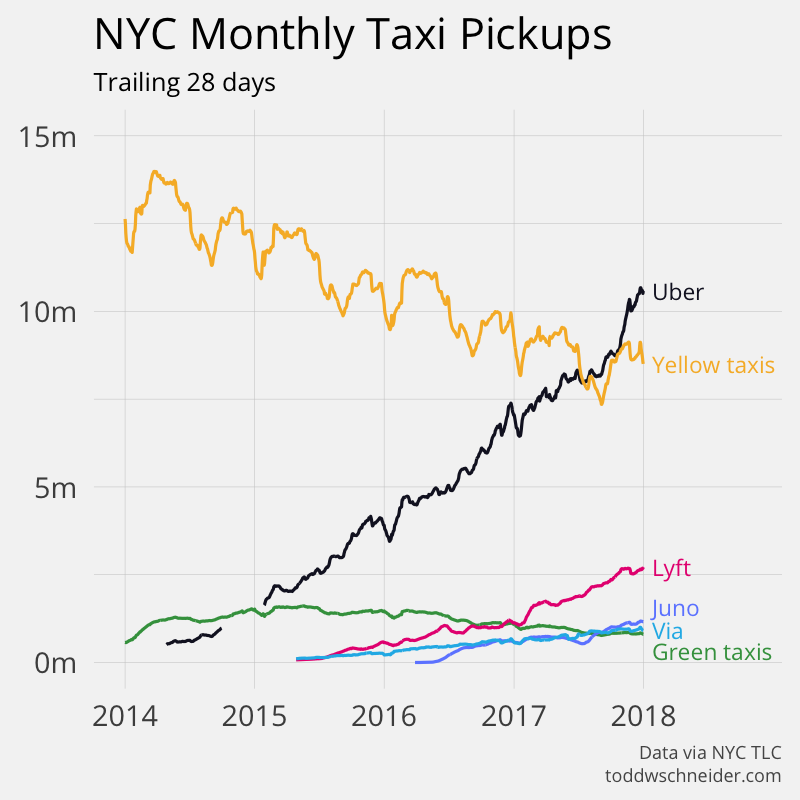
\includegraphics[width=5.33in]{figure/totals_by_car_type} 

}

\caption{NYC Monthly Taxi Pickups}\label{fig:totals-by-car-type}
\end{figure}
As shown in Figure 1.1 (Schneider, 2015), the number of New York City
yellow taxi trips has been consistently declining for about 4 years, and
the number of Uber and Lyft trips keep increasing. In 2017, for the
first time, the total number of monthly Uber trips exceeded the number
of yellow taxi trips.

Some studies have shown how competitive Uber and Lyft are. In 2017, Uber
and Lyft registered vehicles outnumbered NYC yellow cabs by 4 to 1
(Sugar, 2017). Even though yellow cabs used to be the most popular
street-hail transportation service in New York City, passengers nowadays
tend to choose the more convenient options, ride-hailing apps (Hu,
2017).

Data scientists from the University of Cambridge in the UK and the
University of Namur in Belgium found that yellow taxi rides are on
average \$1.40 cheaper than Uber X, which is one type of economy ride
service offered by Uber (H. Staff, 2018). Moreover, Uber appears more
expensive for trips that are cheaper than \$35, and less expensive than
yellow taxi ride for trips that are more expensive than \$35. Therefore,
for short trips, taking a taxi is more affordable (Vsevolod Salnikov,
2015).

Apps, such as Openstreetcab, that compare the price of Uber and taxi
trips are designed to help customers to compare the fares of different
transportations (Vsevolod Salnikov, 2015).

\subsection{\texorpdfstring{\texttt{etl} R
package}{etl R package}}\label{etl-r-package}

Working with taxi trip data is not an easy task, because of the large
size of the taxi trip datasets (Whitford, 2017). Loading these datasets
into \textbf{R} environment takes a long time and might crush an
\textbf{R} session. Taxi trip datasets are classified as medium data,
because they are too big to be processed in an \textbf{R} session but
not too big to be saved on a hard drive.

To better understand how difficult it was to work with medium data in
\textbf{R}, I tried to calculate a simple average of total amount of
taxi fare that passengers paid to New York City yellow taxi drivers in
2017. I was not able to get a simple average by using \textbf{R} on my
laptop which has 8 GB of physical memory, because the total amount of
yellow taxi 2017 data is about 10 GB. I was not even able to load all
2017 data into \textbf{R} environment. It used to be impossible to
answer ``simple'' questions related to New York City yellow taxi with
the help of \textbf{R}.

The \texttt{etl} \textbf{R} package creates a user-friendly platform
that allows \textbf{R} users to easily work with medium data with the
\emph{extract}, \emph{transform}, \emph{load} framework, which is
commonly known as ETL in computing. The \texttt{ETL} process has been
set up (B. S. Baumer, 2017) in \textbf{R} to facilitate \texttt{etl}
operations for medium data, and it is designed to work with any general
data set. Packages that are specific to particular data sets are needed
to be written in order to better work with complex medium-sized data
sets.

\section{Contribution}\label{contribution}

This thesis has two main components: the \texttt{nyctaxi} \textbf{R}
package, which helps users to analyze the New York City street-hail
services' data in \textbf{R}, and recommendations for taxi drivers,
passengers, and TLC officials. In addition to the two main parts, we
focus on making all analysis and visualizations in this study
reproducible.

\subsection{\texorpdfstring{`nyctaxi'
Package}{nyctaxi Package}}\label{nyctaxi-package}

\texttt{nyctaxi} is an \textbf{R} package that help users to easily get
access to New York City Taxi, Uber and Lyft trip data (B. S. Baumer,
2017). This package facilitates ETL to deal with medium data that are
too big to store in memory on a laptop. Users are given the option to
choose specific years and months as the input parameters of the three
ETL functions, and a connection to a populated SQL database will be
returned as the output. Users do not need to learn SQL queries, since
all user interaction is in \textbf{R}.
\begin{center}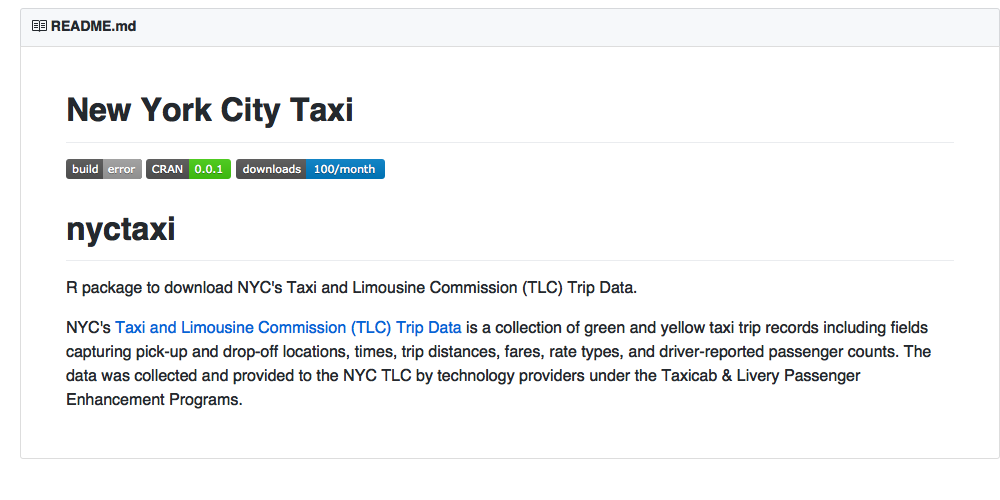
\includegraphics[width=5.88in]{figure/nyctaxi-page} \end{center}

\subsection{Reproducible Research}\label{reproducible-research}

In
\texttt{R\ Markdown:\ Integrating\ A\ Reproducible\ Analysis\ Tool\ into\ Introductory\ Statistics},
the authors have presented experimental and statistical evidence that
\emph{R Markdown} replaced the antiquated and hard-to-reproduce
\texttt{copy-and-paste\ workflow}, and makes creating fully-reproducible
statistical analysis straight-forward (B. Baumer, Cetinkaya-Rundel,
Bray, Loi, \& Horton, 2014).

Reproducible research and open source are two main points of emphasis in
this honors project. As scholars place more emphasis on the
reproducibility of research studies, it is essential for us to make our
data and code openly available for people to redo the analysis.

\texttt{knitr} (Xie, 2018) and Github are used in this project to make
the study reproducible, ranging from the initial data source to the
\texttt{nyctaxi} package to the statistical data analysis. We used an
\textbf{R} package called \texttt{thesisdown} to typeset this paper.
This tool allows authors to create reproducible and dynamic technical
report in \textbf{R} Markdown. It also allows users to embed \textbf{R}
code and interactive applications, and output into PDF, Word, ePub, or
gitbook documents. \texttt{thesisdown} helps users to efficiently put
together any paper with similar format (Solomon, 2016).

Github is used to store the scripts for \texttt{nyctaxi} and this
thesis. \texttt{nyctaxi} is available on CRAN for people to download and
install (W. P. Li, Baumer, \& Trang Le, 2017), and the source code for
data analysis in this thesis is available under the Github account of
the author so that scholars can easily access the information that they
are interested in. In terms of tables, figures, and anything included in
the Appendix attached to this thesis, scripts that are used to generate
them are included in the Github repository.

\subsection{Recommendations for taxi drivers, passengers, and TLC
officials}\label{recommendations-for-taxi-drivers-passengers-and-tlc-officials}

In Chapters 3 to 5, we analyze what taxi drivers, passengers, and TLC
officials want and we try to find ways for them to achieve their goals.

NYC Taxi drivers want to make the profit. Our analysis has suggested
that taxi passengers are sympathetic with the drivers who have to suffer
the congestion in New York City, and pay more tips during rush hours.

Taxi passengers want the cheapest and most convenient way of
transportation. We created a Shiny App for passengers to choose a
pick-up zone of their interest and then decide when is the most
favorable time for them to travel from that zone to any of the three
airports in New York.

TLC wants to protect both taxi drivers and passengers, and it creates
policies to make NYC taxi more accessible to consumers and taxi drivers
enjoy their work. We suggest New York City TLC to modify the fare on
rainy or snowy days to incentive taxicab drivers to pick up more trips
in order to make taking a street hail vehicle on average more affordable
on rainy days for passengers.

\chapter{\texorpdfstring{Data and \texttt{nyctaxi}
Package}{Data and nyctaxi Package}}\label{chapter2}

\section{Data and Storage}\label{data-and-storage}

The \texttt{nyctaxi} \textbf{R} package allows users to download, clean,
and load data into SQL databases. There are four types of data that are
available for users to get access to: trip level yellow taxi data from
2009 to the most recent month, trip level green taxi data from August
2013 to the most recent month, Uber pick-up data from April to September
2014 and from Janaury to June 2015, and weekly-aggregated Lyft trip data
from 2016 to the most recent week (W. P. Li et al., 2017).

\subsection{Yellow Taxi}\label{yellow-taxi-1}

The total size of all yellow taxi trip data \texttt{csv} files (from Jan
2010 to Dec 2016) is 191.38 GB, and NYC yellow taxi trip data from Jan
2009 to the most recent month can be found on the NYC Taxi \& Limousine
Commission (TLC) website (N. T. Staff, 2009b). The data were collected
and provided to the NYC TLC by technology providers authorized under the
Taxicab \& Livery Passenger Enhancement Programs (TPEP/LPEP).

The yellow taxi trip records include the following fields: pick-up and
drop-off dates/times, pick-up and drop-off locations, trip distances,
itemized fares, rate types, payment types, and driver-reported passenger
counts.

\subsection{Green Taxi}\label{green-taxi-1}

The total size of green taxi trip data \texttt{csv} files (from Aug 2013
to Dec 2016) is 7.8 GB, and green taxi trip data from Aug 2013 to the
most recent month can be downloaded from NYC Taxi \& Limousine
Commission (TLC). (N. T. Staff, 2009b) Green taxi trip records include
the same variables as yellow taxi trip records.

\subsection{TLC Summary Report}\label{tlc-summary-report}

The New York City TLC publishes summary reports that include aggregate
statistics about taxi, Uber, and Lyft usage. These are in addition to
the trip-level data; although the summary reports contain much less
detail, they're updated more frequently, which provides a more current
glimpse into the state of the cutthroat NYC taxi market. (N. T. Staff,
2009a)

In addition, the trip level NYC Uber data only covers two periods, from
April to September 2014 and from January to June 2015. However, the
summary reports cover weekly-aggregated data from 2015 to the most
recent week (N. T. Staff, 2009c) (Figure 2.1).
\begin{figure}[h]

{\centering 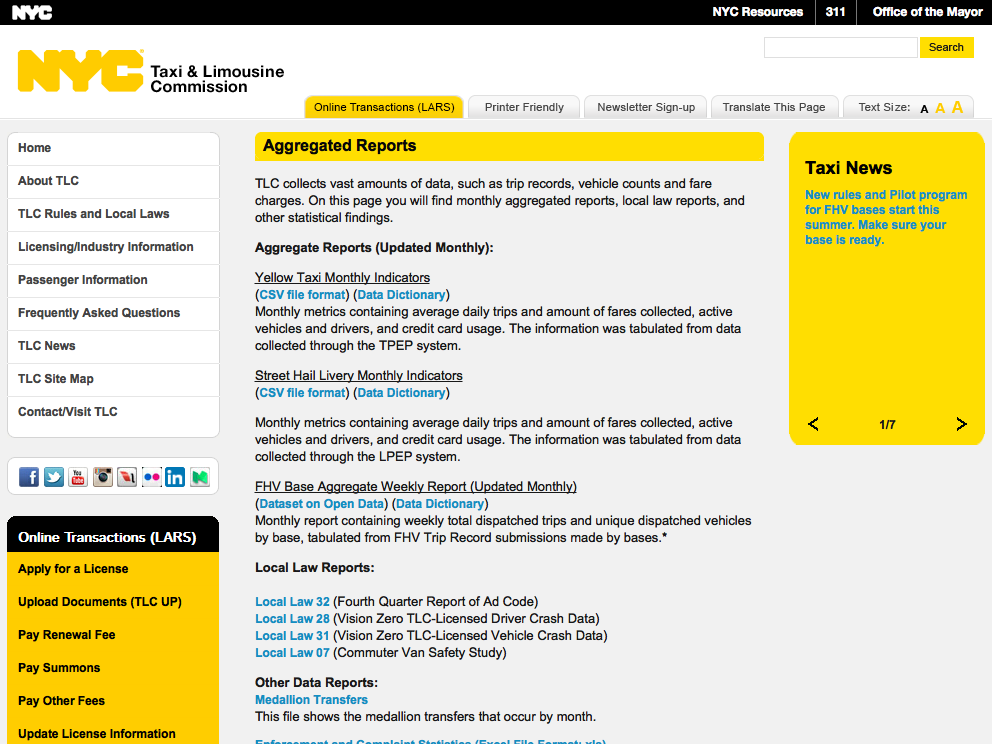
\includegraphics[width=5.84in]{figure/a-report} 

}

\caption{NYC Taxi and Limousine Commission Aggregated Reports}\label{fig:a-report}
\end{figure}
The data can be accessed by using the following commands:
\begin{itemize}
\tightlist
\item
  Yellow taxi data
\end{itemize}
\begin{Shaded}
\begin{Highlighting}[]
\KeywordTok{download.file}\NormalTok{(}\StringTok{"http://www.nyc.gov/html/tlc/downloads/csv/data_reports_}
\StringTok{              monthly_indicators_yellow.csv"}\NormalTok{, }
              \DataTypeTok{destfile =} \StringTok{"~/Desktop/yellow_monthly_data.csv"}\NormalTok{)}
\end{Highlighting}
\end{Shaded}
\begin{itemize}
\tightlist
\item
  Uber and Lyft data
\end{itemize}
\begin{Shaded}
\begin{Highlighting}[]
\KeywordTok{download.file}\NormalTok{(}\StringTok{"http://data.cityofnewyork.us/api/views/2v9c-2k7f/rows.csv}
\StringTok{              ?accessType=DOWNLOAD"}\NormalTok{, }
              \DataTypeTok{destfile =} \StringTok{"~/Desktop/fhv_weekly_data.csv"}\NormalTok{)}
\end{Highlighting}
\end{Shaded}
\subsection{Uber}\label{uber-1}

The total size of Uber pick-up data (from Apr to Sep 2014 and from Jan
to June 2015) is 900 MB, and thanks to FiveThirtyEight (FiveThirtyEight,
2015) who obtained the data from NYC TLC by submitting a Freedom of
Information Law (FOIL) request on July 20, 2015, these data are now open
to public.

The 2014 Uber data contains 4 variables: \texttt{Date/Time} (the date
and time of the Uber pick-up), \texttt{Lat} (the latitude of the Uber
pick-up), \texttt{Lon} (the longitude of the Uber pick-up), and
\texttt{Base} (the TLC base company code affiliated with the Uber
pickup).

The 2015 Uber data contains 4 variables: \texttt{Dispatching\_base\_num}
(the TLC base company code of the base that dispatched the Uber),
\texttt{Pickup\_date} (the date of the Uber pick-up),
\texttt{Affiliated\_base\_num} (the TLC base company code affiliated
with the Uber pickup), and \texttt{locationID} (the pick-up location ID
affiliated with the Uber pickup).

NYC Open Data also provides weekly-aggregated Uber pick-up data from
2015 to the most recent month (N. O. Staff, 2015b).

\subsection{Lyft}\label{lyft-1}

The total size of weekly-aggregated Lyft trip data (from Jan 2015 to Dec
2016) is 914.9 MB, and these data are open to public and
weekly-aggregated Lyft data from 2015 to the most recent week can be
found on NYC OpenData website (N. O. Staff, 2015a).

\subsection{Data Storage}\label{data-storage}

The total size of all \texttt{csv} files of the four services is about
200 GB, and a laptop usually has 8 GB of physical memory. Limited memory
constrains the amount of data that can be loaded by a personal computer
at one time. When users load data into \textbf{R} environment,
\textbf{R} keeps them in memory; when the amount of data loaded into
\textbf{R} environment gets close to the limit of a computer's memory,
\textbf{R} becomes unresponsive or force quit the current session.
Therefore, better ways to work with data that takes more space than 8 GB
is needed. Comparing to RAM, hard disk is often used to store
medium-sized data, because it is affordable and are designed for storing
large items permanently. However, retrieving data from hard drives is
about 1,000,000 times slower (Zhnag, 2017).

\section{\texorpdfstring{\texttt{etl} and \texttt{nyctaxi}
Packages}{etl and nyctaxi Packages}}\label{etl-and-nyctaxi-packages}

\texttt{etl} is the parent package of \texttt{nyctaxi}. \texttt{etl}
provides a framework that allows \textbf{R} users to work with medium
data without any knowledge in SQL database. Users can run SQL queries by
using \texttt{dplyr} commands in \textbf{R} and choose to only return
the final result, which could be a summary table, from SQL database into
\textbf{R} Environment in order to avoid \textbf{R} from crashing. The
user interaction takes place solely within \textbf{R}.

\texttt{etl} framework has three operations -Extract, Transfer, and
Load- which bring real-time data into local or remote SQL databases.
Users can specify which type of SQL database they prefer to connect to.
\texttt{etl}-dependent packages, such as \texttt{nyctaxi}, make medium
data more accessible to a wider audience (B. Baumer et al., 2014).

\texttt{nyctaxi} (Figure 2.2) was initially designed to work with New
York City taxi data, but later on Uber and Lyft data were added and the
ETL functions are modified to be specialized in working with these data.
This package compiles three major sources of hail service in New York
City so that it is convenient for users to compare and contrast the
performance of these three services (W. P. Li et al., 2017).

This package inherits functions from many packages:
\begin{itemize}
\tightlist
\item
  \texttt{etl} (B. S. Baumer, 2017)
\item
  \texttt{dplyr} (Wickham, Francois, Henry, \& Müller, 2017)
\item
  \texttt{DBI} (R Special Interest Group on Databases (R-SIG-DB),
  Wickham, \& Müller, 2018)
\item
  \texttt{rlang} (Henry \& Wickham, 2018)
\item
  \texttt{lubridate} (Grolemund \& Wickham, 2011)
\item
  \texttt{leaflet} (Cheng, Karambelkar, \& Xie, 2017)
\item
  \texttt{stringr} (Wickham, 2018)
\end{itemize}
SQL database can store medium data and it takes less time to retrieve
data from a SQL database than from a hard disk. Since SQL databases are
good tools for medium data analysis, ETL functions build connection to a
SQL database at the back end and convert \textbf{R} code automatically
into SQL queries and send them to the SQL database to get data tables
containing data of each hail service. Thus, users do not need to have
any knowledge of SQL queries and they can draw in any subsets of the
data from the SQL database in \textbf{R}.
\begin{figure}[h]

{\centering 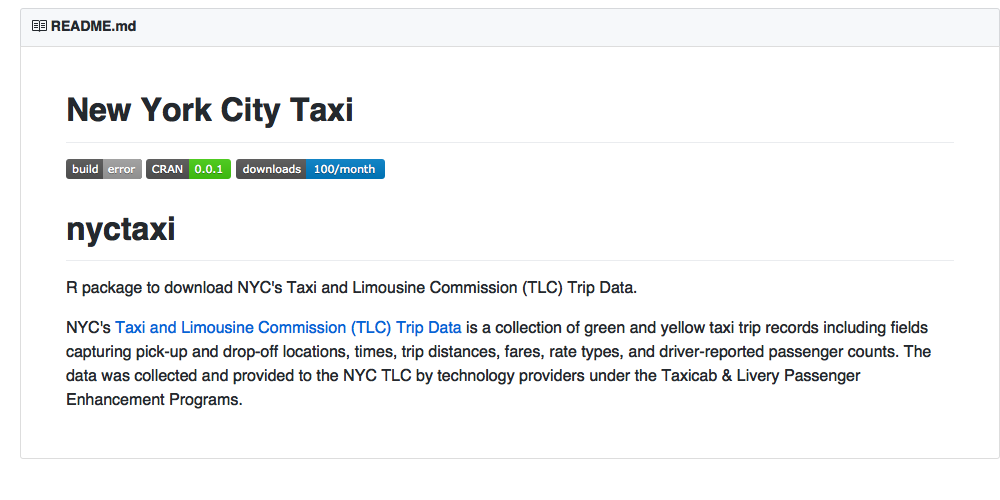
\includegraphics[width=5.88in]{figure/nyctaxi-page} 

}

\caption{`nyctaxi` package GitHub Repository}\label{fig:nyctaxi-page}
\end{figure}
In general, \texttt{etl\_extract.etl\_nyctaxi()} function downloads data
of the four types of hail service data (yellow taxi, green taxi, Uber,
and Lyft) from the corresponding sources.
\texttt{etl\_transform.etl\_nyctaxi()} uses different techniques to
clean all four types of data to get then ready for the next step.
\texttt{etl\_load.etl\_nyctaxi()} loads the data user selected to a SQL
database.

The Comprehensive \textbf{R} Archive Network (CRAN) is a collection of
sites that carry identical material, consisting of the \textbf{R}
distributions, the contributed extensions, documentation for \textbf{R},
and binaries (C. Staff, 1993). \texttt{nyctaxi} \textbf{R} package lives
on CRAN, and it can be installed as follows:
\begin{Shaded}
\begin{Highlighting}[]
\KeywordTok{install.packages}\NormalTok{(}\StringTok{"nyctaxi"}\NormalTok{)}
\end{Highlighting}
\end{Shaded}
Users need to create an \texttt{etl} object in order to apply the etl
operations to it, and only the name of the SQL database, working
directory, and type of SQL database need to be specified during
initialization. If the type of SQL database is not specified, a local
RSQLite database will be generated as default.
\begin{Shaded}
\begin{Highlighting}[]
\NormalTok{db <-}\StringTok{ }\KeywordTok{src_mysql}\NormalTok{(}\StringTok{"nyctaxi"}\NormalTok{, }\DataTypeTok{user =} \StringTok{"urname"}\NormalTok{, }\DataTypeTok{host =} \StringTok{"host"}\NormalTok{, }
                \DataTypeTok{password =} \StringTok{"pw"}\NormalTok{)}
\NormalTok{taxi <-}\StringTok{ }\KeywordTok{etl}\NormalTok{(}\StringTok{"nyctaxi"}\NormalTok{, }\DataTypeTok{dir =} \StringTok{"~/Desktop/nyctaxi"}\NormalTok{, db)}
\end{Highlighting}
\end{Shaded}
In the example above, a folder called \texttt{nyctaxi} is created on the
desktop and a connection to a MySQL database is generated. In the
procession of initialization, two subfolders, \texttt{raw} and
\texttt{load}, are also created under the directory the user specifies.
The \texttt{raw} folder stores data downloaded from online open sources,
and \texttt{load} folder stores cleaned CSV data files that are ready to
be loaded into SQL database. The ETL framework keeps data directly
scraped from online data sources in their original forms. In this way,
the original data is always available to users in case data corruption
happens in later stages.

After an \texttt{etl} object is created (\texttt{taxi} is the
\texttt{etl} object in this case), four parameters are needed to specify
the data that users want: (1) \texttt{obj}: an \texttt{etl} object; (2)
\texttt{years}: a numeric vector giving the years, and the default is
the most recent year; (3) \texttt{months}: a numeric vector giving the
months, and the default is \texttt{1:12}; (4) \texttt{type}: a character
variable giving the type of data the user wants to download. There are
four types corresponding to four street-hail services: \texttt{yellow},
\texttt{green}, \texttt{uber}, and \texttt{lyft}. The default is
\texttt{yellow}.

\subsection{\texorpdfstring{Taxi zone shapefile attached to nyctaxi
\textbf{R}
package}{Taxi zone shapefile attached to nyctaxi R package}}\label{taxi-zone-shapefile-attached-to-nyctaxi-r-package}

Two datasets are attached to \texttt{nyctaxi}. The first one is called
\texttt{taxi\_zone\_lookup}, and this dataset contains information, such
as taxi zone location IDs, location names, and corresponding boroughs
for each ID (N. T. Staff, 2009b). A shapefile containing the boundaries
for the taxi zones, \texttt{taxi\_zones}, is also included in the
package for users to do spatial analysis. This shapefile is publicly
accessible on NYC TLC's website (N. T. Staff, 2009b).
\begin{figure}[h]

{\centering 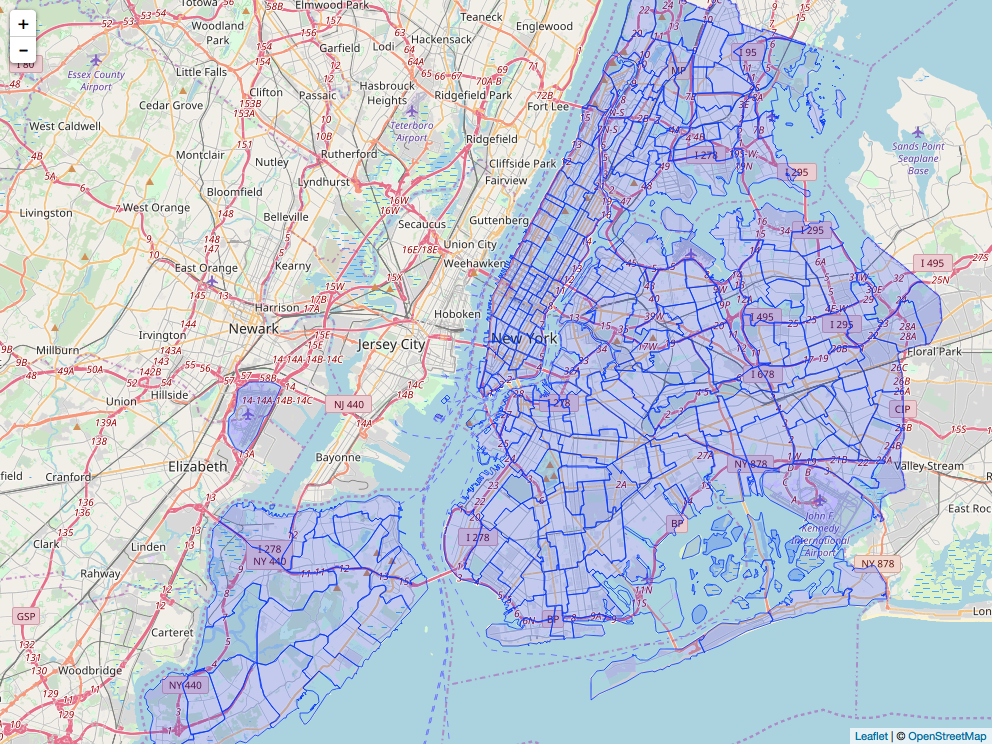
\includegraphics[width=5.84in]{figure/zonemap} 

}

\caption{NYC Taxi Zone Map}\label{fig:zonemap}
\end{figure}
Visualizations similar to Figure \ref{fig:zonemap} can be generated with
the shapefile.

\section{Extract-Transform-Load}\label{extract-transform-load}

\subsection{Extract}\label{extract}

\texttt{etl\_extract.etl\_nyctaxi()} allows users to download New York
City yellow taxi, green taxi, Uber, and Lyft data from the corresponding
data sources. It takes the \texttt{years}, \texttt{months}, and
\texttt{type} parameters and download the New York City taxi data
specified by users. New York City Yellow and Green Taxi data are updated
on NYC Taxi \& Limousine Commission (TLC) website on a monthly basis.
\begin{Shaded}
\begin{Highlighting}[]
\NormalTok{taxi }\OperatorTok\StringTok{ }
\StringTok{   }\KeywordTok{etl_extract}\NormalTok{(}\DataTypeTok{years =} \DecValTok{2014}\OperatorTok{:}\DecValTok{2016}\NormalTok{, }\DataTypeTok{months =} \DecValTok{1}\OperatorTok{:}\DecValTok{12}\NormalTok{, }
               \DataTypeTok{type =} \KeywordTok{c}\NormalTok{(}\StringTok{"yellow"}\NormalTok{, }\StringTok{"green"}\NormalTok{))}
\end{Highlighting}
\end{Shaded}
Uber trip record data is static and small, so we decided to only give
users the options to download either all data from April to September,
2014 or all Uber trip records from January to June, 2015 at once. We do
not give users the option to download Uber data by month, since the
total size of all trip-level data from 2014 and 2015 are small.
\begin{Shaded}
\begin{Highlighting}[]
\NormalTok{taxi }\OperatorTok\StringTok{ }
\StringTok{   }\KeywordTok{etl_extract}\NormalTok{(}\DataTypeTok{years =} \DecValTok{2014}\OperatorTok{:}\DecValTok{2016}\NormalTok{, }\DataTypeTok{months =} \DecValTok{1}\OperatorTok{:}\DecValTok{12}\NormalTok{, }
               \DataTypeTok{type =} \KeywordTok{c}\NormalTok{(}\StringTok{"uber"}\NormalTok{))}
\end{Highlighting}
\end{Shaded}
Lyft data is updated on NYC Open Data website on a weekly basis. Since
the weekly-aggregated data is tiny and only data later than 2014 is
available, we decided to only allow users to download Lyft data by year.
We do not give users the option to download Lyft data by month, since
trip records are weekly-aggregated.
\begin{Shaded}
\begin{Highlighting}[]
\NormalTok{taxi }\OperatorTok\StringTok{ }
\StringTok{   }\KeywordTok{etl_extract}\NormalTok{(}\DataTypeTok{years =} \DecValTok{2014}\OperatorTok{:}\DecValTok{2016}\NormalTok{, }\DataTypeTok{months =} \DecValTok{1}\OperatorTok{:}\DecValTok{12}\NormalTok{, }
               \DataTypeTok{type =} \KeywordTok{c}\NormalTok{(}\StringTok{"lyft"}\NormalTok{))}
\end{Highlighting}
\end{Shaded}
The default \texttt{years} is the current year, and the default
\texttt{months} are all twelve months. The default type of
transportation is \texttt{yellow}. When an invalid month is entered,
warning message will suggest users to reconsider their choice and select
a new set of month.

An utility function, \texttt{download\_nyc\_data()}, was written to be
used in \texttt{etl\_extract.etl\_nyctaxi()} to make this function more
concise (Appendix A).

\subsection{Transform}\label{transform}

\texttt{etl\_transform.etl\_nyctaxi()} allows users to transform the
data into cleaned formats, and it utilizes different data cleaning
techniques when it transforms data for each transportation type. In
general, it cleans the data and creates a new \texttt{csv} file in the
\texttt{load} directory to store the cleaned data. It helps us to retain
and protect raw data from being modified or destroyed. Users are allowed
to specify the month of interest in order to only transform data from
certain months. This functionality helps people to be more efficient
with their use of time by only transforming months of data that are
needed in later steps.

By default, it takes the current year yellow taxi trip records data
files, and saves copies of them in the \texttt{load} directory. It skips
the cleaning step, because the raw yellow taxi data downloaded from TLC
is already in a desired format with all variables correctly labelled.
\begin{Shaded}
\begin{Highlighting}[]
\NormalTok{taxi }\OperatorTok\StringTok{ }
\StringTok{   }\KeywordTok{etl_transform}\NormalTok{(}\DataTypeTok{years =} \DecValTok{2014}\OperatorTok{:}\DecValTok{2016}\NormalTok{, }\DataTypeTok{months =} \DecValTok{1}\OperatorTok{:}\DecValTok{12}\NormalTok{, }
                 \DataTypeTok{type =} \KeywordTok{c}\NormalTok{(}\StringTok{"yellow"}\NormalTok{, }\StringTok{"green"}\NormalTok{, }\StringTok{"uber"}\NormalTok{, }\StringTok{"lyft"}\NormalTok{))}
\end{Highlighting}
\end{Shaded}
There are a few main transformations that are done by this function:

\subsubsection{Green Taxi -- Extra Blank Row and
Column}\label{green-taxi-extra-blank-row-and-column}

Green Taxi monthly data from August 2013 to the most recent month
besides 2015 all have a blank second row in the \texttt{csv} files.
Similar to this problem, Green Taxi data from 2013, 2014, and 2015 all
have an extra blank column attached to the right-most column. These
blank rows and columns cause problems in the later stage when users want
to load data into SQL database. In order to get Green Taxi data ready
for the \texttt{load} phase, we used the \texttt{system()} function in
\textbf{R} to invoke the \texttt{cut} Terminal command specified to
remove the blank rows and columns.

\subsubsection{Uber Data -- Reconciling Inconsistent
Filenames}\label{uber-data-reconciling-inconsistent-filenames}

Uber only released over 4.5 million data records from April to September
2014 and 14.3 million records from January to June 2015. Information of
different sets of variables are released for 2014 and 2015, and
variables have different naming convention. When users want to download
data from both years, variables are renamed so that data from both years
can be consolidated into one big dataset with consistent variable names.

\subsubsection{Uber Data -- Reconciling Inconsistent Data
Formats}\label{uber-data-reconciling-inconsistent-data-formats}

The data type of \texttt{Date/Time} variable in Uber datasets is
originally encoded as \texttt{character}. In order to enable it to be
recognized as \texttt{timestamp} by \textbf{R}, we use \texttt{ymd\_hms}
in \texttt{lubridate} (Grolemund \& Wickham, 2011) to transform date
time to \texttt{POSIXct} objects.

\subsubsection{Optimizing I/O Process}\label{optimizing-io-process}

Improving file input and output processes is an important part of
\texttt{etl\_transform}. \texttt{data.table} (Dowle \& Srinivasan, 2017)
only takes half of the time to read from and write into datasets
comparing to \texttt{readr} (Wickham, Hester, \& Francois, 2017).
Therefore, \texttt{etl\_transform} uses \texttt{fread()} and
\texttt{fwrite()} from \texttt{data.table} instead of \texttt{read\_csv}
or \texttt{write\_csv} from \texttt{readr} to reduce the data processing
time (Zhang, 2017).

\subsection{Load}\label{load}

\texttt{etl\_load.etl\_nyctaxi()} allows users to load New York City
yellow taxi, green taxi, Uber, and Lyft data into different data tables
in a SQL database. It populates a SQL database with data cleaned by
\texttt{etl\_transform}.
\begin{Shaded}
\begin{Highlighting}[]
\NormalTok{taxi }\OperatorTok\StringTok{ }
\StringTok{   }\KeywordTok{etl_load}\NormalTok{(}\DataTypeTok{years =} \DecValTok{2014}\OperatorTok{:}\DecValTok{2016}\NormalTok{, }\DataTypeTok{months =} \DecValTok{1}\OperatorTok{:}\DecValTok{12}\NormalTok{, }
            \DataTypeTok{type =} \KeywordTok{c}\NormalTok{(}\StringTok{"yellow"}\NormalTok{, }\StringTok{"green"}\NormalTok{, }\StringTok{"uber"}\NormalTok{, }\StringTok{"lyft"}\NormalTok{))}
\end{Highlighting}
\end{Shaded}
\subsection{SQL Database
Initialization}\label{sql-database-initialization}

\texttt{init.mysql} is written under \texttt{nyctaxi} to help users to
set up five basic table structures for MySQL database.
\texttt{yellow\_old} is created for Yellow Taxi data that are prior to
July 2016, and \texttt{yellow} is created for data later than June 2016.
There are two tables created for yellow taxi data because NYC TLC
changed the variables included in yellow taxi datasets in July 2016.
Table \texttt{green}, \texttt{uber}, and \texttt{lyft} are also
initiated for green taxi, Uber and Lyft data.

\texttt{etl\_init()} can be run after a database connection is built to
process to process \texttt{init.mysql} to initialize a MySQL database,
and default columns with the correct variable names and types defined
will be automatically generated.
\begin{Shaded}
\begin{Highlighting}[]
\NormalTok{taxi }\OperatorTok
\StringTok{  }\KeywordTok{etl_init}\NormalTok{()}
\end{Highlighting}
\end{Shaded}
In order to increase the query speed at the data analysis stage,
\texttt{KEY}s are created for multiple variables for each
transportation. Since there is no variable containing unique value for
each observation, no primary variable is needed. Using \texttt{KEY}s in
data analysis query can speed up the query process.

Due to the large size of Yellow Taxi datasets, \texttt{yellow\_old} and
\texttt{yellow} are partitioned into subgroups by \texttt{year}. When we
need to run a query on data from a specific year, having partitions
allows MySQL to directly find the data specified without filtering on
every single row. It speeds up the query process.
\begin{figure}[h]

{\centering 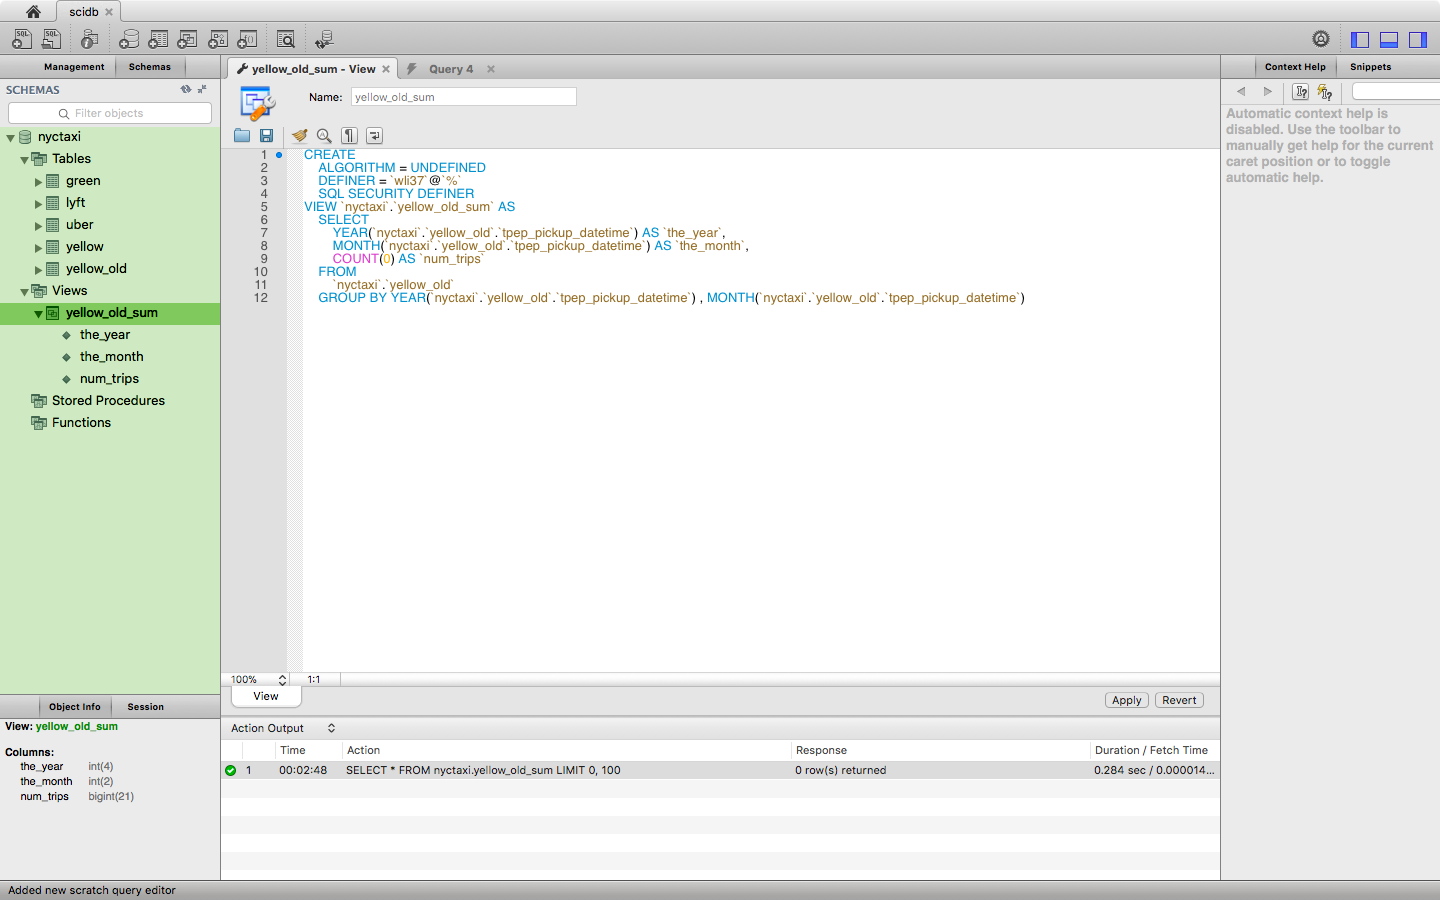
\includegraphics[width=5.76in]{figure/mysql_view} 

}

\caption{MySQL View}\label{fig:mysql-view}
\end{figure}
A \texttt{VIEW} called \texttt{yellow\_old\_sum} is also created to
generate a summary table for the number of Yellow Taxi trips in each
month.

\section{New York City Taxicab and E-hail Services
Summary}\label{new-york-city-taxicab-and-e-hail-services-summary}
\begin{figure}[h]

{\centering 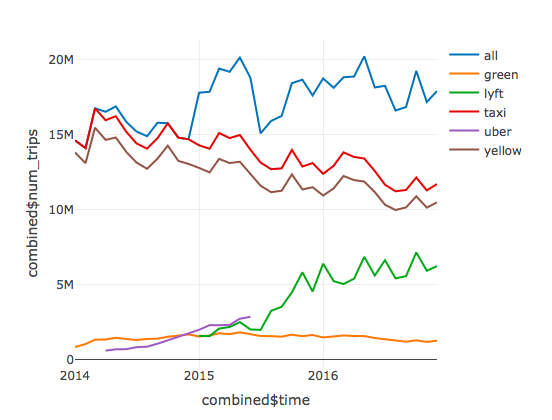
\includegraphics[width=5.75in]{figure/Num_trips_summary} 

}

\caption{Summary of Number of trips Made by 4 Types of Transportations between 2014 and 2016 in NYC}\label{fig:num-trips-summary}
\end{figure}
Figure \ref{fig:num-trips-summary} is a summary of total number of trips
made by all 4 types of transportations that are available to users from
2014 to 2016. In order to generate this summary, I combined trip-level
yellow and green taxi data from TLC website (N. T. Staff, 2009b) and
weekly Uber (N. O. Staff, 2015b) and Lyft data from NYC OpenData (N. O.
Staff, 2015a). Trip-level Uber data that can be accessed by using the
\texttt{nyctaxi} package is not used in the creation of Figure
\ref{fig:num-trips-summary} because of the limited ranges of dates where
the Uber trip-level data is available.

Data used in Figure \ref{fig:num-trips-summary} can be accessed by
running the code below:
\begin{itemize}
\tightlist
\item
  Yellow and green taxi trip data
\end{itemize}
\begin{Shaded}
\begin{Highlighting}[]
\NormalTok{taxi }\OperatorTok
\StringTok{  }\KeywordTok{etl_extract}\NormalTok{(}\DataTypeTok{years =} \DecValTok{2014}\OperatorTok{:}\DecValTok{2016}\NormalTok{, }\DataTypeTok{months =} \DecValTok{1}\OperatorTok{:}\DecValTok{12}\NormalTok{, }\DataTypeTok{type =} \KeywordTok{c}\NormalTok{(}\StringTok{"yellow"}\NormalTok{, }\StringTok{"green"}\NormalTok{)) }\OperatorTok
\StringTok{  }\KeywordTok{etl_transform}\NormalTok{(}\DataTypeTok{years =} \DecValTok{2014}\OperatorTok{:}\DecValTok{2016}\NormalTok{, }\DataTypeTok{months =} \DecValTok{1}\OperatorTok{:}\DecValTok{12}\NormalTok{, }\DataTypeTok{type =} \KeywordTok{c}\NormalTok{(}\StringTok{"yellow"}\NormalTok{, }\StringTok{"green"}\NormalTok{)) }\OperatorTok
\StringTok{  }\KeywordTok{etl_load}\NormalTok{(}\DataTypeTok{years =} \DecValTok{2014}\OperatorTok{:}\DecValTok{2016}\NormalTok{, }\DataTypeTok{months =} \DecValTok{1}\OperatorTok{:}\DecValTok{12}\NormalTok{, }\DataTypeTok{type =} \KeywordTok{c}\NormalTok{(}\StringTok{"yellow"}\NormalTok{, }\StringTok{"green"}\NormalTok{)) }
\end{Highlighting}
\end{Shaded}
\begin{itemize}
\tightlist
\item
  Uber weekly data
\end{itemize}
\begin{Shaded}
\begin{Highlighting}[]
\KeywordTok{download.file}\NormalTok{(}\StringTok{"https://data.cityofnewyork.us/resource/gt3n-7ri6.csv"}\NormalTok{,}
              \DataTypeTok{destfile =} \StringTok{"~/Desktop/uber_weekly_data.csv"}\NormalTok{)}
\end{Highlighting}
\end{Shaded}
\begin{itemize}
\tightlist
\item
  Lyft weekly data
\end{itemize}
\begin{Shaded}
\begin{Highlighting}[]
\NormalTok{taxi }\OperatorTok
\StringTok{  }\KeywordTok{etl_extract}\NormalTok{(}\DataTypeTok{years =} \DecValTok{2014}\OperatorTok{:}\DecValTok{2016}\NormalTok{, }\DataTypeTok{months =} \DecValTok{1}\OperatorTok{:}\DecValTok{12}\NormalTok{, }\DataTypeTok{type =} \StringTok{"lyft"}\NormalTok{) }\OperatorTok
\StringTok{  }\KeywordTok{etl_transform}\NormalTok{(}\DataTypeTok{years =} \DecValTok{2014}\OperatorTok{:}\DecValTok{2016}\NormalTok{, }\DataTypeTok{months =} \DecValTok{1}\OperatorTok{:}\DecValTok{12}\NormalTok{, }\DataTypeTok{type =} \StringTok{"lyft"}\NormalTok{) }\OperatorTok
\StringTok{  }\KeywordTok{etl_load}\NormalTok{(}\DataTypeTok{years =} \DecValTok{2014}\OperatorTok{:}\DecValTok{2016}\NormalTok{, }\DataTypeTok{months =} \DecValTok{1}\OperatorTok{:}\DecValTok{12}\NormalTok{, }\DataTypeTok{type =} \StringTok{"lyft"}\NormalTok{) }
\end{Highlighting}
\end{Shaded}
\section{Source Code}\label{source-code}

\subsection{ETL Extract}\label{etl-extract}
\begin{Shaded}
\begin{Highlighting}[]
\NormalTok{etl_extract.etl_nyctaxi <-}\StringTok{ }
\StringTok{  }\ControlFlowTok{function}\NormalTok{(obj, }
\DataTypeTok{years =} \KeywordTok{as.numeric}\NormalTok{(}\KeywordTok{format}\NormalTok{(}\KeywordTok{Sys.Date}\NormalTok{(),}\StringTok{'%Y'}\NormalTok{)), }
                                    \DataTypeTok{months =} \DecValTok{1}\OperatorTok{:}\DecValTok{12}\NormalTok{, }
                                    \DataTypeTok{type  =} \StringTok{"yellow"}\NormalTok{,...) \{}
  \CommentTok{#TAXI YELLOW-------------------------}
\NormalTok{  taxi_yellow <-}\StringTok{ }\ControlFlowTok{function}\NormalTok{(obj, years, months,...) \{}
    \KeywordTok{message}\NormalTok{(}\StringTok{"Extracting raw yellow taxi data..."}\NormalTok{)}
\NormalTok{    remote <-}\StringTok{ }\NormalTok{etl}\OperatorTok{::}\KeywordTok{valid_year_month}\NormalTok{(years, months, }
    \DataTypeTok{begin =} \StringTok{"2009-01-01"}\NormalTok{) }\OperatorTok
\StringTok{      }\KeywordTok{mutate_}\NormalTok{(}\DataTypeTok{src =} 
  \OperatorTok{~}\KeywordTok{file.path}\NormalTok{(}\StringTok{"https://s3.amazonaws.com/nyc-tlc/trip+data"}\NormalTok{, }
                               \KeywordTok{paste0}\NormalTok{(}\StringTok{"yellow"}\NormalTok{, }\StringTok{"_tripdata_"}\NormalTok{, year, }\StringTok{"-"}\NormalTok{,}
\NormalTok{                      stringr}\OperatorTok{::}\KeywordTok{str_pad}\NormalTok{(month, }\DecValTok{2}\NormalTok{, }\StringTok{"left"}\NormalTok{, }\StringTok{"0"}\NormalTok{), }\StringTok{".csv"}\NormalTok{))) }
    \KeywordTok{tryCatch}\NormalTok{(}\DataTypeTok{expr =}\NormalTok{ etl}\OperatorTok{::}\KeywordTok{smart_download}\NormalTok{(obj, remote}\OperatorTok{$}\NormalTok{src, ...),}
             \DataTypeTok{error =} \ControlFlowTok{function}\NormalTok{(e)\{}\KeywordTok{warning}\NormalTok{(e)\}, }
             \DataTypeTok{finally =} \KeywordTok{warning}\NormalTok{(}\StringTok{"Only the following data are availabel on}
\StringTok{                                TLC: Yellow taxi data: 2009 Jan - }
\StringTok{                               last month"}\NormalTok{))\} }
  \CommentTok{#TAXI GREEN----------------------}
\NormalTok{  taxi_green <-}\StringTok{ }\ControlFlowTok{function}\NormalTok{(obj, years, months,...) \{}
    \KeywordTok{message}\NormalTok{(}\StringTok{"Extracting raw green taxi data..."}\NormalTok{)}
\NormalTok{    remote <-}\StringTok{ }\NormalTok{etl}\OperatorTok{::}\KeywordTok{valid_year_month}\NormalTok{(years, months, }\DataTypeTok{begin =} \StringTok{"2013-08-01"}\NormalTok{) }\OperatorTok
\StringTok{      }\KeywordTok{mutate_}\NormalTok{(}\DataTypeTok{src =} 
                \OperatorTok{~}\KeywordTok{file.path}\NormalTok{(}\StringTok{"https://s3.amazonaws.com/nyc-tlc/trip+data"}\NormalTok{, }
                               \KeywordTok{paste0}\NormalTok{(}\StringTok{"green"}\NormalTok{, }\StringTok{"_tripdata_"}\NormalTok{, year, }\StringTok{"-"}\NormalTok{,}
\NormalTok{                          stringr}\OperatorTok{::}\KeywordTok{str_pad}\NormalTok{(month, }\DecValTok{2}\NormalTok{, }\StringTok{"left"}\NormalTok{, }\StringTok{"0"}\NormalTok{), }\StringTok{".csv"}\NormalTok{)))}
    \KeywordTok{tryCatch}\NormalTok{(}\DataTypeTok{expr =}\NormalTok{ etl}\OperatorTok{::}\KeywordTok{smart_download}\NormalTok{(obj, remote}\OperatorTok{$}\NormalTok{src, ...),}
             \DataTypeTok{error =} \ControlFlowTok{function}\NormalTok{(e)\{}\KeywordTok{warning}\NormalTok{(e)\}, }
             \DataTypeTok{finally =} \KeywordTok{warning}\NormalTok{(}\StringTok{"Only the following data are availabel on TLC:}
\StringTok{                               Green taxi data: 2013 Aug - last month"}\NormalTok{))\} }
  \CommentTok{#UBER--------------------------------}
\NormalTok{  uber <-}\StringTok{ }\ControlFlowTok{function}\NormalTok{(obj, years, months,...) \{}
    \KeywordTok{message}\NormalTok{(}\StringTok{"Extracting raw uber data..."}\NormalTok{)}
\NormalTok{    raw_month_}\DecValTok{2014}\NormalTok{ <-}\StringTok{ }\NormalTok{etl}\OperatorTok{::}\KeywordTok{valid_year_month}\NormalTok{(}\DataTypeTok{years =} \DecValTok{2014}\NormalTok{, }\DataTypeTok{months =} \DecValTok{4}\OperatorTok{:}\DecValTok{9}\NormalTok{)}
\NormalTok{    raw_month_}\DecValTok{2015}\NormalTok{ <-}\StringTok{ }\NormalTok{etl}\OperatorTok{::}\KeywordTok{valid_year_month}\NormalTok{(}\DataTypeTok{years =} \DecValTok{2015}\NormalTok{, }\DataTypeTok{months =} \DecValTok{1}\OperatorTok{:}\DecValTok{6}\NormalTok{)}
\NormalTok{    raw_month <-}\StringTok{ }\KeywordTok{bind_rows}\NormalTok{(raw_month_}\DecValTok{2014}\NormalTok{, raw_month_}\DecValTok{2015}\NormalTok{)}
\NormalTok{    path =}\StringTok{ "https://raw.githubusercontent.com/}
\StringTok{    fivethirtyeight/uber-tlc-foil-response/master/uber-trip-data"}
\NormalTok{    remote <-}\StringTok{ }\NormalTok{etl}\OperatorTok{::}\KeywordTok{valid_year_month}\NormalTok{(years, months)}
\NormalTok{    remote_small <-}\StringTok{ }\KeywordTok{intersect}\NormalTok{(raw_month, remote)}
    \ControlFlowTok{if}\NormalTok{ (}\DecValTok{2015} \OperatorTok\StringTok{ }\NormalTok{remote_small}\OperatorTok{$}\NormalTok{year }\OperatorTok{&&}\StringTok{ }\OperatorTok{!}\NormalTok{(}\DecValTok{2014} \OperatorTok\StringTok{ }\NormalTok{remote_small}\OperatorTok{$}\NormalTok{year))\{}
      \CommentTok{#download 2015 data}
      \KeywordTok{message}\NormalTok{(}\StringTok{"Downloading Uber 2015 data..."}\NormalTok{)}
\NormalTok{      etl}\OperatorTok{::}\KeywordTok{smart_download}\NormalTok{(obj, }\StringTok{"https://github.com/fivethirtyeight/}
\StringTok{                          uber-tlc-foil-response/raw/master/}
\StringTok{                    uber-trip-data/uber-raw-data-janjune-15.csv.zip"}\NormalTok{,...)\}}
    \ControlFlowTok{else} \ControlFlowTok{if}\NormalTok{ (}\DecValTok{2015} \OperatorTok\StringTok{ }\NormalTok{remote_small}\OperatorTok{$}\NormalTok{year }\OperatorTok{&&}\StringTok{ }\DecValTok{2014} \OperatorTok\StringTok{ }\NormalTok{remote_small}\OperatorTok{$}\NormalTok{year) \{}
      \CommentTok{#download 2015 data}
      \KeywordTok{message}\NormalTok{(}\StringTok{"Downloading Uber 2015 data..."}\NormalTok{)}
\NormalTok{      etl}\OperatorTok{::}\KeywordTok{smart_download}\NormalTok{(obj, }\StringTok{"https://github.com/fivethirtyeight/}
\StringTok{                        uber-tlc-foil-response/raw/master/uber-trip-data}
\StringTok{                          /uber-raw-data-janjune-15.csv.zip"}\NormalTok{,...)}
      \CommentTok{#download 2014 data}
\NormalTok{      small <-}\StringTok{ }\NormalTok{remote_small }\OperatorTok
\StringTok{        }\KeywordTok{filter_}\NormalTok{(}\OperatorTok{~}\NormalTok{year }\OperatorTok{==}\StringTok{ }\DecValTok{2014}\NormalTok{) }\OperatorTok
\StringTok{        }\KeywordTok{mutate_}\NormalTok{(}\DataTypeTok{month_abb =} \OperatorTok{~}\KeywordTok{tolower}\NormalTok{(month.abb[month]),}
                \DataTypeTok{src =} \OperatorTok{~}\KeywordTok{file.path}\NormalTok{(path,}
                \KeywordTok{paste0}\NormalTok{(}\StringTok{"uber-raw-data-"}\NormalTok{,month_abb,}
                \KeywordTok{substr}\NormalTok{(year,}\DecValTok{3}\NormalTok{,}\DecValTok{4}\NormalTok{),}\StringTok{".csv"}\NormalTok{)))}
      \KeywordTok{message}\NormalTok{(}\StringTok{"Downloading Uber 2014 data..."}\NormalTok{)}
\NormalTok{      etl}\OperatorTok{::}\KeywordTok{smart_download}\NormalTok{(obj, small}\OperatorTok{$}\NormalTok{src,...) }
\NormalTok{    \} }\ControlFlowTok{else} \ControlFlowTok{if}\NormalTok{ (}\DecValTok{2014} \OperatorTok\StringTok{ }\NormalTok{remote_small}\OperatorTok{$}\NormalTok{year }\OperatorTok{&&}\StringTok{ }
\StringTok{    }\OperatorTok{!}\NormalTok{(}\DecValTok{2015} \OperatorTok\StringTok{ }\NormalTok{remote_small}\OperatorTok{$}\NormalTok{year)) \{}
      \KeywordTok{message}\NormalTok{(}\StringTok{"Downloading Uber 2014 data..."}\NormalTok{)}
      \CommentTok{#file paths}
\NormalTok{      small <-}\StringTok{ }\NormalTok{remote_small }\OperatorTok
\StringTok{        }\KeywordTok{mutate_}\NormalTok{(}\DataTypeTok{month_abb =} 
                  \OperatorTok{~}\KeywordTok{tolower}\NormalTok{(month.abb[month]),}
                \DataTypeTok{src =} \OperatorTok{~}\KeywordTok{file.path}\NormalTok{(path,}
                \KeywordTok{paste0}\NormalTok{(}\StringTok{"uber-raw-data-"}\NormalTok{,month_abb,}
                \KeywordTok{substr}\NormalTok{(year,}\DecValTok{3}\NormalTok{,}\DecValTok{4}\NormalTok{),}\StringTok{".csv"}\NormalTok{)))}
\NormalTok{      etl}\OperatorTok{::}\KeywordTok{smart_download}\NormalTok{(obj, small}\OperatorTok{$}\NormalTok{src,...)\}}
    \ControlFlowTok{else}\NormalTok{ \{}\KeywordTok{warning}\NormalTok{(}\StringTok{"The Uber data you requested are }
\StringTok{                  not currently available. Only data}
\StringTok{                  from 2014/04-2014/09 and 2015/01-}
\StringTok{                  2015/06 are available..."}\NormalTok{)\}}
\NormalTok{    \} }
  \CommentTok{#LYFT----------------------------------}
\NormalTok{  lyft <-}\StringTok{ }\ControlFlowTok{function}\NormalTok{(obj, years, months,...)\{}
    \KeywordTok{message}\NormalTok{(}\StringTok{"Extracting raw lyft data..."}\NormalTok{)}
    \CommentTok{#check if the week is valid}
\NormalTok{    valid_months <-}\StringTok{ }\NormalTok{etl}\OperatorTok{::}\KeywordTok{valid_year_month}\NormalTok{(years, months,}
    \DataTypeTok{begin =} \StringTok{"2015-01-01"}\NormalTok{)}
\NormalTok{    base_url =}\StringTok{ "https://data.cityofnewyork.us/}
\StringTok{    resource/edp9-qgv4.csv"}
\NormalTok{    valid_months <-}\StringTok{ }\NormalTok{valid_months }\OperatorTok
\StringTok{      }\KeywordTok{mutate_}\NormalTok{(}\DataTypeTok{new_filenames =} 
                \OperatorTok{~}\KeywordTok{paste0}\NormalTok{(}\StringTok{"lyft-"}\NormalTok{, year, }\StringTok{".csv"}\NormalTok{)) }\OperatorTok
\StringTok{      }\KeywordTok{mutate_}\NormalTok{(}\DataTypeTok{drop =} \OtherTok{TRUE}\NormalTok{)}
    \CommentTok{#only keep one data set per year}
\NormalTok{    year <-}\StringTok{ }\NormalTok{valid_months[}\DecValTok{1}\NormalTok{,}\DecValTok{1}\NormalTok{]}
\NormalTok{    n <-}\StringTok{ }\KeywordTok{nrow}\NormalTok{(valid_months)}
    \ControlFlowTok{for}\NormalTok{ (i }\ControlFlowTok{in} \DecValTok{2}\OperatorTok{:}\NormalTok{n) \{}
      \ControlFlowTok{if}\NormalTok{(year }\OperatorTok{==}\StringTok{ }\NormalTok{valid_months[i}\OperatorTok{-}\DecValTok{1}\NormalTok{,}\DecValTok{1}\NormalTok{]) \{}
\NormalTok{        valid_months[i,}\DecValTok{6}\NormalTok{] <-}\StringTok{ }\OtherTok{FALSE}
\NormalTok{        year <-}\StringTok{ }\NormalTok{valid_months[i}\OperatorTok{+}\DecValTok{1}\NormalTok{,}\DecValTok{1}\NormalTok{]}
\NormalTok{      \} }\ControlFlowTok{else}\NormalTok{ \{}
\NormalTok{        valid_months[i,}\DecValTok{6}\NormalTok{] <-}\StringTok{ }\OtherTok{TRUE}
\NormalTok{        year <-}\StringTok{ }\NormalTok{valid_months[i}\OperatorTok{+}\DecValTok{1}\NormalTok{,}\DecValTok{1}\NormalTok{]\}}
\NormalTok{      \}}
\NormalTok{    row_to_keep =}\StringTok{ }\NormalTok{valid_months}\OperatorTok{$}\NormalTok{drop}
\NormalTok{    valid_months <-}\StringTok{ }\NormalTok{valid_months[row_to_keep,]}
    
    \CommentTok{#download lyft files, try two different methods}
\NormalTok{    first_try<-}\KeywordTok{tryCatch}\NormalTok{(}
      \KeywordTok{download_nyc_data}\NormalTok{(obj, base_url, valid_months}\OperatorTok{$}\NormalTok{year, }
      \DataTypeTok{n =} \DecValTok{50000}\NormalTok{, }\DataTypeTok{names =}\NormalTok{ valid_months}\OperatorTok{$}\NormalTok{new_filenames),}
      \DataTypeTok{error =} \ControlFlowTok{function}\NormalTok{(e)\{}\KeywordTok{warning}\NormalTok{(e)\},}
      \DataTypeTok{finally =} \StringTok{'method = "libcurl" fails'}\NormalTok{)}
\NormalTok{  \}}
  
  \ControlFlowTok{if}\NormalTok{ (type }\OperatorTok{==}\StringTok{ "yellow"}\NormalTok{)\{}\KeywordTok{taxi_yellow}\NormalTok{(obj, years, months,...)\} }
  \ControlFlowTok{else} \ControlFlowTok{if}\NormalTok{ (type }\OperatorTok{==}\StringTok{ "green"}\NormalTok{)\{}\KeywordTok{taxi_green}\NormalTok{(obj, years, months,...)\}}
  \ControlFlowTok{else} \ControlFlowTok{if}\NormalTok{ (type }\OperatorTok{==}\StringTok{ "uber"}\NormalTok{)\{}\KeywordTok{uber}\NormalTok{(obj, years, months,...)\}}
  \ControlFlowTok{else} \ControlFlowTok{if}\NormalTok{ (type }\OperatorTok{==}\StringTok{ "lyft"}\NormalTok{)\{}\KeywordTok{lyft}\NormalTok{(obj, years, months,...)\}}
  \ControlFlowTok{else}\NormalTok{ \{}\KeywordTok{message}\NormalTok{(}\StringTok{"The type you chose does not exit..."}\NormalTok{)\}}
  
  \KeywordTok{invisible}\NormalTok{(obj)}
\NormalTok{\}}
\end{Highlighting}
\end{Shaded}
\subsection{ETL Transform}\label{etl-transform}
\begin{Shaded}
\begin{Highlighting}[]
\NormalTok{opts_chunk}\OperatorTok{$}\KeywordTok{set}\NormalTok{(}\DataTypeTok{tidy.opts=}\KeywordTok{list}\NormalTok{(}\DataTypeTok{width.cutoff=}\DecValTok{60}\NormalTok{))}
\NormalTok{etl_transform.etl_nyctaxi <-}\StringTok{ }\ControlFlowTok{function}\NormalTok{(obj, }
                          \DataTypeTok{years =} \KeywordTok{as.numeric}\NormalTok{(}\KeywordTok{format}\NormalTok{(}\KeywordTok{Sys.Date}\NormalTok{(),}\StringTok{'%Y'}\NormalTok{)), }
                          \DataTypeTok{months =} \DecValTok{1}\OperatorTok{:}\DecValTok{12}\NormalTok{, }
                          \DataTypeTok{type  =} \StringTok{"yellow"}\NormalTok{,...) \{}
  \CommentTok{#TAXI YELLOW-----------------------------}
\NormalTok{  taxi_yellow <-}\StringTok{ }\ControlFlowTok{function}\NormalTok{(obj, years, months) \{}
    \KeywordTok{message}\NormalTok{(}\StringTok{"Transforming yellow taxi data from raw to }
\StringTok{            load directory..."}\NormalTok{)}
    \CommentTok{#create a df of file path of the files that the user wants to transform}
\NormalTok{    remote <-}\StringTok{ }\NormalTok{etl}\OperatorTok{::}\KeywordTok{valid_year_month}\NormalTok{(years, months, }
    \DataTypeTok{begin =} \StringTok{"2009-01-01"}\NormalTok{) }\OperatorTok
\StringTok{      }\KeywordTok{mutate_}\NormalTok{(}\DataTypeTok{src =} \OperatorTok{~}\KeywordTok{file.path}\NormalTok{(}\KeywordTok{attr}\NormalTok{(obj, }\StringTok{"raw_dir"}\NormalTok{), }
      \KeywordTok{paste0}\NormalTok{(}\StringTok{"yellow"}\NormalTok{, }\StringTok{"_tripdata_"}\NormalTok{, year, }\StringTok{"-"}\NormalTok{,}
\NormalTok{      stringr}\OperatorTok{::}\KeywordTok{str_pad}\NormalTok{(month, }\DecValTok{2}\NormalTok{, }\StringTok{"left"}\NormalTok{, }\StringTok{"0"}\NormalTok{), }\StringTok{".csv"}\NormalTok{))) }
    \CommentTok{#create a df of file path of the files that are in the raw directory}
\NormalTok{    src <-}\StringTok{ }\KeywordTok{list.files}\NormalTok{(}\KeywordTok{attr}\NormalTok{(obj, }\StringTok{"raw_dir"}\NormalTok{), }\StringTok{"yellow"}\NormalTok{, }\DataTypeTok{full.names =} \OtherTok{TRUE}\NormalTok{)}
\NormalTok{    src_small <-}\StringTok{ }\KeywordTok{intersect}\NormalTok{(src, remote}\OperatorTok{$}\NormalTok{src)}
    \CommentTok{#Move the files}
\NormalTok{    in_raw <-}\StringTok{ }\KeywordTok{basename}\NormalTok{(src_small)}
\NormalTok{    in_load <-}\StringTok{ }\KeywordTok{basename}\NormalTok{(}\KeywordTok{list.files}\NormalTok{(}\KeywordTok{attr}\NormalTok{(obj, }\StringTok{"load_dir"}\NormalTok{), }\StringTok{"yellow"}\NormalTok{, }
    \DataTypeTok{full.names =} \OtherTok{TRUE}\NormalTok{))}
\NormalTok{    file_remian <-}\StringTok{ }\KeywordTok{setdiff}\NormalTok{(in_raw,in_load)}
    \KeywordTok{file.copy}\NormalTok{(}\KeywordTok{file.path}\NormalTok{(}\KeywordTok{attr}\NormalTok{(obj, }\StringTok{"raw_dir"}\NormalTok{),file_remian),}
              \KeywordTok{file.path}\NormalTok{(}\KeywordTok{attr}\NormalTok{(obj, }\StringTok{"load_dir"}\NormalTok{),file_remian) )\}}
  \CommentTok{#TAXI GREEN-----------------------------}
\NormalTok{  taxi_green <-}\StringTok{ }\ControlFlowTok{function}\NormalTok{(obj, years, months) \{}
    \KeywordTok{message}\NormalTok{(}\StringTok{"Transforming green taxi data from raw }
\StringTok{            to load directory..."}\NormalTok{)}
    \CommentTok{#create a df of file path of the files that the user wants to transform}
\NormalTok{    remote <-}\StringTok{ }\NormalTok{etl}\OperatorTok{::}\KeywordTok{valid_year_month}\NormalTok{(years, months, }
    \DataTypeTok{begin =} \StringTok{"2013-08-01"}\NormalTok{) }\OperatorTok
\StringTok{      }\KeywordTok{mutate_}\NormalTok{(}\DataTypeTok{src =} \OperatorTok{~}\KeywordTok{file.path}\NormalTok{(}\KeywordTok{attr}\NormalTok{(obj, }\StringTok{"raw_dir"}\NormalTok{), }
      \KeywordTok{paste0}\NormalTok{(}\StringTok{"green"}\NormalTok{, }\StringTok{"_tripdata_"}\NormalTok{, year, }\StringTok{"-"}\NormalTok{,}
\NormalTok{      stringr}\OperatorTok{::}\KeywordTok{str_pad}\NormalTok{(month, }\DecValTok{2}\NormalTok{, }\StringTok{"left"}\NormalTok{, }\StringTok{"0"}\NormalTok{), }\StringTok{".csv"}\NormalTok{))) }
    \CommentTok{#create a df of file path of the files that are in the raw directory}
\NormalTok{    src <-}\StringTok{ }\KeywordTok{list.files}\NormalTok{(}\KeywordTok{attr}\NormalTok{(obj, }\StringTok{"raw_dir"}\NormalTok{), }\StringTok{"green"}\NormalTok{, }\DataTypeTok{full.names =} \OtherTok{TRUE}\NormalTok{)}
\NormalTok{    src_small <-}\StringTok{ }\KeywordTok{intersect}\NormalTok{(src, remote}\OperatorTok{$}\NormalTok{src)}
    \CommentTok{#Clean the green taxi data files}
    \CommentTok{#get rid of 2nd blank row}
    \ControlFlowTok{if}\NormalTok{ (}\KeywordTok{length}\NormalTok{(src_small) }\OperatorTok{==}\StringTok{ }\DecValTok{0}\NormalTok{)\{}
      \KeywordTok{message}\NormalTok{(}\StringTok{"The files you requested are not available }
\StringTok{              in the raw directory."}\NormalTok{)}
\NormalTok{    \} }\ControlFlowTok{else}\NormalTok{\{}
      \CommentTok{#a list of the ones that have a 2nd blank row}
\NormalTok{      remote_green_}\DecValTok{1}\NormalTok{ <-}\StringTok{ }\NormalTok{remote }\OperatorTok\StringTok{ }\KeywordTok{filter_}\NormalTok{(}\OperatorTok{~}\NormalTok{year }\OperatorTok{!=}\StringTok{ }\DecValTok{2015}\NormalTok{)}
\NormalTok{      src_small_green_}\DecValTok{1}\NormalTok{ <-}\StringTok{ }\KeywordTok{intersect}\NormalTok{(src, remote_green_}\DecValTok{1}\OperatorTok{$}\NormalTok{src)}
      \CommentTok{# check that the sys support command line, }
      \CommentTok{#and then remove the blank 2nd row}
      \ControlFlowTok{if}\NormalTok{(}\KeywordTok{length}\NormalTok{(src_small_green_}\DecValTok{1}\NormalTok{) }\OperatorTok{!=}\StringTok{ }\DecValTok{0}\NormalTok{) \{}
        \ControlFlowTok{if}\NormalTok{ (.Platform}\OperatorTok{$}\NormalTok{OS.type }\OperatorTok{==}\StringTok{ "unix"}\NormalTok{)\{}
\NormalTok{          cmds_}\DecValTok{1}\NormalTok{ <-}\StringTok{ }\KeywordTok{paste}\NormalTok{(}\StringTok{"sed -i -e '2d'"}\NormalTok{, src_small_green_}\DecValTok{1}\NormalTok{)}
          \KeywordTok{lapply}\NormalTok{(cmds_}\DecValTok{1}\NormalTok{, system)}
\NormalTok{        \} }\ControlFlowTok{else}\NormalTok{ \{}
          \KeywordTok{message}\NormalTok{(}\StringTok{"Windows system does not }
\StringTok{          currently support removing the 2nd blank row}
\StringTok{          in the green taxi datasets. This might affect }
\StringTok{          loading data into SQL..."}\NormalTok{)\}}
\NormalTok{        \}}\ControlFlowTok{else}\NormalTok{ \{}
          \StringTok{"You did not request for any }
\StringTok{          green taxi data, or all the green}
\StringTok{          taxi data you requested are cleaned."}\NormalTok{\}}
      \CommentTok{#fix column number}
\NormalTok{      remote_green_}\DecValTok{2}\NormalTok{ <-}\StringTok{ }\NormalTok{remote }\OperatorTok
\StringTok{        }\KeywordTok{filter_}\NormalTok{(}\OperatorTok{~}\NormalTok{year }\OperatorTok\StringTok{ }\KeywordTok{c}\NormalTok{(}\DecValTok{2013}\NormalTok{, }\DecValTok{2014}\NormalTok{, }\DecValTok{2015}\NormalTok{)) }\OperatorTok
\StringTok{        }\KeywordTok{mutate_}\NormalTok{(}\DataTypeTok{keep =} 
                  \OperatorTok{~}\KeywordTok{ifelse}\NormalTok{(year }\OperatorTok\StringTok{ }\KeywordTok{c}\NormalTok{(}\DecValTok{2013}\NormalTok{,}\DecValTok{2014}\NormalTok{), }\DecValTok{20}\NormalTok{,}\DecValTok{21}\NormalTok{),}
                \DataTypeTok{new_file =} 
                  \OperatorTok{~}\KeywordTok{paste0}\NormalTok{(}\StringTok{"green_tripdata_"}\NormalTok{, year, }\StringTok{"_"}\NormalTok{, }
\NormalTok{                      stringr}\OperatorTok{::}\KeywordTok{str_pad}\NormalTok{(month, }\DecValTok{2}\NormalTok{, }\StringTok{"left"}\NormalTok{, }\StringTok{"0"}\NormalTok{),}
                                   \StringTok{".csv"}\NormalTok{))}
\NormalTok{      src_small_green_}\DecValTok{2}\NormalTok{ <-}\StringTok{ }\KeywordTok{intersect}\NormalTok{(src, remote_green_}\DecValTok{2}\OperatorTok{$}\NormalTok{src)}
\NormalTok{      src_small_green_2_df <-}\StringTok{ }\KeywordTok{data.frame}\NormalTok{(src_small_green_}\DecValTok{2}\NormalTok{) }
      \KeywordTok{names}\NormalTok{(src_small_green_2_df) <-}\StringTok{ "src"}
\NormalTok{      src_small_green_2_df <-}\StringTok{ }\KeywordTok{inner_join}\NormalTok{(src_small_green_2_df, }
\NormalTok{      remote_green_}\DecValTok{2}\NormalTok{, }\DataTypeTok{by =} \StringTok{"src"}\NormalTok{)}
\NormalTok{      src_small_green_2_df <-}\StringTok{ }\NormalTok{src_small_green_2_df }\OperatorTok
\StringTok{        }\KeywordTok{mutate}\NormalTok{(}\DataTypeTok{cmds_2 =} \KeywordTok{paste}\NormalTok{(}\StringTok{"cut -d, -f1-"}\NormalTok{, keep,}\StringTok{" "}\NormalTok{,src, }\StringTok{" > "}\NormalTok{,}
        \KeywordTok{attr}\NormalTok{(obj, }\StringTok{"raw_dir"}\NormalTok{),}\StringTok{"/green_tripdata_"}\NormalTok{, }
\NormalTok{        year, }\StringTok{"_"}\NormalTok{, stringr}\OperatorTok{::}\KeywordTok{str_pad}\NormalTok{(month, }\DecValTok{2}\NormalTok{, }\StringTok{"left"}\NormalTok{, }\StringTok{"0"}\NormalTok{),}\StringTok{".csv"}\NormalTok{, }
        \DataTypeTok{sep =} \StringTok{""}\NormalTok{))}
      \CommentTok{#remove the extra column}
      \ControlFlowTok{if}\NormalTok{(}\KeywordTok{length}\NormalTok{(src_small_green_}\DecValTok{2}\NormalTok{) }\OperatorTok{!=}\StringTok{ }\DecValTok{0}\NormalTok{) \{}
        \ControlFlowTok{if}\NormalTok{ (.Platform}\OperatorTok{$}\NormalTok{OS.type }\OperatorTok{==}\StringTok{ "unix"}\NormalTok{)\{}
          \KeywordTok{lapply}\NormalTok{(src_small_green_2_df}\OperatorTok{$}\NormalTok{cmds_}\DecValTok{2}\NormalTok{, system)\} }
        \ControlFlowTok{else}\NormalTok{ \{}
          \KeywordTok{message}\NormalTok{(}\StringTok{"Windows system does not currently }
\StringTok{          support removing the 2nd blank row }
\StringTok{          in the green taxi datasets. This might }
\StringTok{          affect loading data into SQL..."}\NormalTok{)\}}
\NormalTok{        \}}\ControlFlowTok{else}\NormalTok{ \{}
          \StringTok{"All the green taxi data you}
\StringTok{          requested are in cleaned formats."}\NormalTok{\}}
      \CommentTok{#Find the files paths of the files that need to be transformed}
      \KeywordTok{file.rename}\NormalTok{(}\KeywordTok{file.path}\NormalTok{(}\KeywordTok{dirname}\NormalTok{(src_small_green_2_df}\OperatorTok{$}\NormalTok{src),}
\NormalTok{                            src_small_green_2_df}\OperatorTok{$}\NormalTok{new_file), }
                  \KeywordTok{file.path}\NormalTok{(}\KeywordTok{attr}\NormalTok{(obj, }\StringTok{"load_dir"}\NormalTok{),}
                  \KeywordTok{basename}\NormalTok{(src_small_green_2_df}\OperatorTok{$}\NormalTok{src)))}
      \CommentTok{#Move the files}
\NormalTok{      in_raw <-}\StringTok{ }\KeywordTok{basename}\NormalTok{(src_small)}
\NormalTok{      in_load <-}\StringTok{ }\KeywordTok{basename}\NormalTok{(}\KeywordTok{list.files}\NormalTok{(}\KeywordTok{attr}\NormalTok{(obj, }\StringTok{"load_dir"}\NormalTok{), }
      \StringTok{"green"}\NormalTok{, }\DataTypeTok{full.names =} \OtherTok{TRUE}\NormalTok{))}
\NormalTok{      file_remian <-}\StringTok{ }\KeywordTok{setdiff}\NormalTok{(in_raw,in_load)}
      \KeywordTok{file.copy}\NormalTok{(}\KeywordTok{file.path}\NormalTok{(}\KeywordTok{attr}\NormalTok{(obj, }\StringTok{"raw_dir"}\NormalTok{),file_remian), }
      \KeywordTok{file.path}\NormalTok{(}\KeywordTok{attr}\NormalTok{(obj, }\StringTok{"load_dir"}\NormalTok{),file_remian) )\}\}}
  \CommentTok{#UBER--------------------------------}
\NormalTok{  uber <-}\StringTok{ }\ControlFlowTok{function}\NormalTok{(obj) \{}
    \KeywordTok{message}\NormalTok{(}\StringTok{"Transforming uber data from raw to load directory..."}\NormalTok{)}
    \CommentTok{#creat a list of 2014 uber data file directory}
\NormalTok{    uber14_list <-}\StringTok{ }\KeywordTok{list.files}\NormalTok{(}\DataTypeTok{path =} \KeywordTok{attr}\NormalTok{(obj, }\StringTok{"raw_dir"}\NormalTok{), }
    \DataTypeTok{pattern =} \StringTok{"14.csv"}\NormalTok{)}
\NormalTok{    uber14_list <-}\StringTok{ }\KeywordTok{data.frame}\NormalTok{(uber14_list)}
\NormalTok{    uber14_list <-}\StringTok{ }\NormalTok{uber14_list }\OperatorTok\StringTok{ }\KeywordTok{mutate_}\NormalTok{(}\DataTypeTok{file_path =} 
    \OperatorTok{~}\KeywordTok{file.path}\NormalTok{(}\KeywordTok{attr}\NormalTok{(obj, }\StringTok{"raw_dir"}\NormalTok{), uber14_list))}
\NormalTok{    uber14file <-}\StringTok{ }\KeywordTok{lapply}\NormalTok{(uber14_list}\OperatorTok{$}\NormalTok{file_path, readr}\OperatorTok{::}\NormalTok{read_csv)}
\NormalTok{    n <-}\StringTok{ }\KeywordTok{length}\NormalTok{(uber14file)}
    \ControlFlowTok{if}\NormalTok{ (n }\OperatorTok{==}\StringTok{ }\DecValTok{1}\NormalTok{) \{}
\NormalTok{      uber14 <-}\StringTok{ }\KeywordTok{data.frame}\NormalTok{(uber14file[}\DecValTok{1}\NormalTok{])}
\NormalTok{    \} }\ControlFlowTok{else} \ControlFlowTok{if}\NormalTok{ (n }\OperatorTok{==}\StringTok{ }\DecValTok{2}\NormalTok{) \{}
\NormalTok{      uber14 <-}\StringTok{ }\KeywordTok{bind_rows}\NormalTok{(uber14file[}\DecValTok{1}\NormalTok{], uber14file[}\DecValTok{2}\NormalTok{])}
\NormalTok{    \} }\ControlFlowTok{else} \ControlFlowTok{if}\NormalTok{ (n }\OperatorTok{>}\StringTok{ }\DecValTok{2}\NormalTok{) \{}
\NormalTok{      uber14 <-}\StringTok{ }\KeywordTok{bind_rows}\NormalTok{(uber14file[}\DecValTok{1}\NormalTok{], uber14file[}\DecValTok{2}\NormalTok{])}
      \ControlFlowTok{for}\NormalTok{ (i }\ControlFlowTok{in} \DecValTok{3}\OperatorTok{:}\NormalTok{n)\{uber14 <-}\StringTok{ }\KeywordTok{bind_rows}\NormalTok{(uber14, uber14file[i])\}}
\NormalTok{    \}}
\NormalTok{    substrRight <-}\StringTok{ }\ControlFlowTok{function}\NormalTok{(x, n)\{}\KeywordTok{substr}\NormalTok{(x, }\KeywordTok{nchar}\NormalTok{(x)}\OperatorTok{-}\NormalTok{n}\OperatorTok{+}\DecValTok{1}\NormalTok{, }\KeywordTok{nchar}\NormalTok{(x))\}}
\NormalTok{    uber14_datetime <-}\StringTok{ }\NormalTok{uber14 }\OperatorTok
\StringTok{      }\KeywordTok{mutate}\NormalTok{(}\DataTypeTok{date =} \KeywordTok{gsub}\NormalTok{( }\StringTok{" .*$"}\NormalTok{, }\StringTok{""}\NormalTok{, }\StringTok{`}\DataTypeTok{Date/Time}\StringTok{`}\NormalTok{), }
      \DataTypeTok{len_date =} \KeywordTok{nchar}\NormalTok{(date), }
             \DataTypeTok{time =} \KeywordTok{sub}\NormalTok{(}\StringTok{'.*}\CharTok{\textbackslash{}\textbackslash{}}\StringTok{ '}\NormalTok{, }\StringTok{''}\NormalTok{, }\StringTok{`}\DataTypeTok{Date/Time}\StringTok{`}\NormalTok{))}
\NormalTok{    uber14_datetime <-}\StringTok{ }\NormalTok{uber14_datetime }\OperatorTok
\StringTok{      }\KeywordTok{mutate}\NormalTok{(}\DataTypeTok{month =} 
               \KeywordTok{substr}\NormalTok{(}\StringTok{`}\DataTypeTok{Date/Time}\StringTok{`}\NormalTok{, }\DecValTok{1}\NormalTok{, }\DecValTok{1}\NormalTok{),}
             \DataTypeTok{day =} \KeywordTok{ifelse}\NormalTok{(len_date }\OperatorTok{==}\StringTok{ }\DecValTok{8}\NormalTok{, }
             \KeywordTok{substr}\NormalTok{(}\StringTok{`}\DataTypeTok{Date/Time}\StringTok{`}\NormalTok{, }\DecValTok{3}\NormalTok{,}\DecValTok{3}\NormalTok{),}\KeywordTok{substr}\NormalTok{(}\StringTok{`}\DataTypeTok{Date/Time}\StringTok{`}\NormalTok{, }\DecValTok{3}\NormalTok{,}\DecValTok{4}\NormalTok{)),}
             \DataTypeTok{pickup_date =} 
\NormalTok{               lubridate}\OperatorTok{::}\KeywordTok{ymd_hms}\NormalTok{(}\KeywordTok{paste0}\NormalTok{(}\StringTok{"2014-"}\NormalTok{, month, }\StringTok{"-"}\NormalTok{, }
\NormalTok{                                         day, }\StringTok{" "}\NormalTok{, time)))}
\NormalTok{    uber14_df <-}\StringTok{ }\NormalTok{uber14_datetime[}\OperatorTok{-}\KeywordTok{c}\NormalTok{(}\DecValTok{1}\NormalTok{,}\DecValTok{5}\OperatorTok{:}\DecValTok{9}\NormalTok{)]}
    
    \CommentTok{#2015}
\NormalTok{    zipped_uberfileURL <-}\StringTok{ }\KeywordTok{file.path}\NormalTok{(}\KeywordTok{attr}\NormalTok{(obj, }\StringTok{"raw_dir"}\NormalTok{),}
    \StringTok{"uber-raw-data-janjune-15.csv.zip"}\NormalTok{)}
\NormalTok{    raw_month_}\DecValTok{2015}\NormalTok{ <-}\StringTok{ }\NormalTok{etl}\OperatorTok{::}\KeywordTok{valid_year_month}\NormalTok{(}\DataTypeTok{years =} \DecValTok{2015}\NormalTok{, }\DataTypeTok{months =} \DecValTok{1}\OperatorTok{:}\DecValTok{6}\NormalTok{)}
\NormalTok{    remote_}\DecValTok{2015}\NormalTok{ <-}\StringTok{ }\NormalTok{etl}\OperatorTok{::}\KeywordTok{valid_year_month}\NormalTok{(years, months)}
\NormalTok{    remote_small_}\DecValTok{2015}\NormalTok{ <-}\StringTok{ }\KeywordTok{inner_join}\NormalTok{(raw_month_}\DecValTok{2015}\NormalTok{, remote_}\DecValTok{2015}\NormalTok{)}
    \ControlFlowTok{if}\NormalTok{(}\KeywordTok{file.exists}\NormalTok{(zipped_uberfileURL) }\OperatorTok{&&}\StringTok{ }
\StringTok{       }\KeywordTok{nrow}\NormalTok{(remote_small_}\DecValTok{2015}\NormalTok{) }\OperatorTok{!=}\StringTok{ }\DecValTok{0}\NormalTok{)\{}
\NormalTok{      utils}\OperatorTok{::}\KeywordTok{unzip}\NormalTok{(}\DataTypeTok{zipfile =}\NormalTok{ zipped_uberfileURL,}\DataTypeTok{unzip =} \StringTok{"internal"}\NormalTok{,}
      \DataTypeTok{exdir =} \KeywordTok{file.path}\NormalTok{(}\KeywordTok{tempdir}\NormalTok{(), }\StringTok{"uber-raw-data-janjune-15.csv.zip"}\NormalTok{))}
\NormalTok{      uber15 <-}\StringTok{ }\NormalTok{readr}\OperatorTok{::}\KeywordTok{read_csv}\NormalTok{(}\KeywordTok{file.path}\NormalTok{(}\KeywordTok{tempdir}\NormalTok{(),}
      \StringTok{"uber-raw-data-janjune-15.csv.zip"}\NormalTok{,}
      \StringTok{"uber-raw-data-janjune-15.csv"}\NormalTok{))\}}
    
    \KeywordTok{names}\NormalTok{(uber14_df) <-}\StringTok{ }\KeywordTok{c}\NormalTok{(}\StringTok{"lat"}\NormalTok{, }\StringTok{"lon"}\NormalTok{, }\StringTok{"affiliated_base_num"}\NormalTok{, }
    \StringTok{"pickup_date"}\NormalTok{)}
    \KeywordTok{names}\NormalTok{(uber15) <-}\StringTok{ }\KeywordTok{tolower}\NormalTok{(}\KeywordTok{names}\NormalTok{(uber15))}
\NormalTok{    uber <-}\StringTok{ }\KeywordTok{bind_rows}\NormalTok{(uber14_df, uber15)}
\NormalTok{    utils}\OperatorTok{::}\KeywordTok{write.csv}\NormalTok{(uber, }\KeywordTok{file.path}\NormalTok{(}\KeywordTok{tempdir}\NormalTok{() ,}\StringTok{"uber.csv"}\NormalTok{))}
    \ControlFlowTok{if}\NormalTok{(}\KeywordTok{nrow}\NormalTok{(uber) }\OperatorTok{!=}\StringTok{ }\DecValTok{0}\NormalTok{) \{}
      \ControlFlowTok{if}\NormalTok{ (.Platform}\OperatorTok{$}\NormalTok{OS.type }\OperatorTok{==}\StringTok{ "unix"}\NormalTok{)\{cmds_}\DecValTok{3}\NormalTok{ <-}\StringTok{ }
\StringTok{      }\KeywordTok{paste}\NormalTok{(}\StringTok{"cut -d, -f2-7"}\NormalTok{,}\KeywordTok{file.path}\NormalTok{(}\KeywordTok{tempdir}\NormalTok{(),}\StringTok{"uber.csv"}\NormalTok{), }\StringTok{" > "}\NormalTok{, }
      \KeywordTok{file.path}\NormalTok{(}\KeywordTok{attr}\NormalTok{(obj, }\StringTok{"load_dir"}\NormalTok{),}\StringTok{"uber.csv"}\NormalTok{))}
        \KeywordTok{lapply}\NormalTok{(cmds_}\DecValTok{3}\NormalTok{, system)}
\NormalTok{      \} }\ControlFlowTok{else}\NormalTok{ \{}
        \KeywordTok{message}\NormalTok{(}\StringTok{"Windows system does not currently }
\StringTok{        support removing the 2nd blank row }
\StringTok{        in the green taxi datasets. This might}
\StringTok{        affect loading data into SQL..."}\NormalTok{)\}}
\NormalTok{      \}}\ControlFlowTok{else}\NormalTok{ \{}
        \StringTok{"You did not request for any }
\StringTok{        green taxi data, or all the green }
\StringTok{        taxi data you requested are cleaned."}\NormalTok{\}}
\NormalTok{    \}}
  \CommentTok{#LYFT--------------------------------}
\NormalTok{  lyft <-}\StringTok{ }\ControlFlowTok{function}\NormalTok{(obj, years, months)\{}
\NormalTok{    valid_months <-}\StringTok{ }\NormalTok{etl}\OperatorTok{::}\KeywordTok{valid_year_month}\NormalTok{(years, }\DataTypeTok{months =} \DecValTok{1}\NormalTok{, }
    \DataTypeTok{begin =} \StringTok{"2015-01-01"}\NormalTok{)}
    \KeywordTok{message}\NormalTok{(}\StringTok{"Transforming lyft data from raw to load directory..."}\NormalTok{)}
\NormalTok{    src <-}\StringTok{ }\KeywordTok{list.files}\NormalTok{(}\KeywordTok{attr}\NormalTok{(obj, }\StringTok{"raw_dir"}\NormalTok{), }\StringTok{"lyft"}\NormalTok{, }\DataTypeTok{full.names =} \OtherTok{TRUE}\NormalTok{)}
\NormalTok{    src_year <-}\StringTok{ }\NormalTok{valid_months }\OperatorTok\StringTok{ }\KeywordTok{distinct_}\NormalTok{(}\OperatorTok{~}\NormalTok{year)}
\NormalTok{    remote <-}\StringTok{ }\KeywordTok{data_frame}\NormalTok{(src)}
\NormalTok{    remote <-}\StringTok{ }\NormalTok{remote }\OperatorTok
\StringTok{      }\KeywordTok{mutate_}\NormalTok{(}\DataTypeTok{lcl =} \OperatorTok{~}\KeywordTok{file.path}\NormalTok{(}\KeywordTok{attr}\NormalTok{(obj, }\StringTok{"load_dir"}\NormalTok{),}\KeywordTok{basename}\NormalTok{(src)),}
              \DataTypeTok{basename =} \OperatorTok{~}\KeywordTok{basename}\NormalTok{(src), }\DataTypeTok{year =} \OperatorTok{~}\KeywordTok{substr}\NormalTok{(basename,}\DecValTok{6}\NormalTok{,}\DecValTok{9}\NormalTok{))}
    \KeywordTok{class}\NormalTok{(remote}\OperatorTok{$}\NormalTok{year) <-}\StringTok{ "numeric"}
\NormalTok{    remote <-}\StringTok{ }\KeywordTok{inner_join}\NormalTok{(remote,src_year, }\DataTypeTok{by =} \StringTok{"year"}\NormalTok{ )}
    \ControlFlowTok{for}\NormalTok{(i }\ControlFlowTok{in} \DecValTok{1}\OperatorTok{:}\KeywordTok{nrow}\NormalTok{(remote)) \{}
\NormalTok{        datafile <-}\StringTok{ }\NormalTok{readr}\OperatorTok{::}\KeywordTok{read_csv}\NormalTok{(remote}\OperatorTok{$}\NormalTok{src[i])}
\NormalTok{        readr}\OperatorTok{::}\KeywordTok{write_delim}\NormalTok{(datafile, }\DataTypeTok{path =}\NormalTok{ remote}\OperatorTok{$}\NormalTok{lcl[i], }
        \DataTypeTok{delim =} \StringTok{"|"}\NormalTok{, }\DataTypeTok{na =} \StringTok{""}\NormalTok{)\}\}}
  
  \CommentTok{#transform the data from raw to load}
  \ControlFlowTok{if}\NormalTok{ (type }\OperatorTok{==}\StringTok{ "yellow"}\NormalTok{)\{}\KeywordTok{taxi_yellow}\NormalTok{(obj, years, months)\} }
  \ControlFlowTok{else} \ControlFlowTok{if}\NormalTok{ (type }\OperatorTok{==}\StringTok{ "green"}\NormalTok{)\{}\KeywordTok{taxi_green}\NormalTok{(obj, years, months)\}}
  \ControlFlowTok{else} \ControlFlowTok{if}\NormalTok{ (type }\OperatorTok{==}\StringTok{ "uber"}\NormalTok{)\{}\KeywordTok{uber}\NormalTok{(obj)\}}
  \ControlFlowTok{else} \ControlFlowTok{if}\NormalTok{ (type }\OperatorTok{==}\StringTok{ "lyft"}\NormalTok{)\{}\KeywordTok{lyft}\NormalTok{(obj, years, months)\}}
  \ControlFlowTok{else}\NormalTok{ \{}\KeywordTok{message}\NormalTok{(}\StringTok{"The type you chose does not exit..."}\NormalTok{)\}}
  
  \KeywordTok{invisible}\NormalTok{(obj)}
\NormalTok{\}}
\end{Highlighting}
\end{Shaded}
\subsection{ETL Load}\label{etl-load}
\begin{Shaded}
\begin{Highlighting}[]
\NormalTok{opts_chunk}\OperatorTok{$}\KeywordTok{set}\NormalTok{(}\DataTypeTok{tidy.opts=}\KeywordTok{list}\NormalTok{(}\DataTypeTok{width.cutoff=}\DecValTok{60}\NormalTok{))}
\NormalTok{etl_load.etl_nyctaxi <-}\StringTok{ }\ControlFlowTok{function}\NormalTok{(obj, }
 \DataTypeTok{years =} \KeywordTok{as.numeric}\NormalTok{(}\KeywordTok{format}\NormalTok{(}\KeywordTok{Sys.Date}\NormalTok{(),}\StringTok{'%Y'}\NormalTok{)), }
                                 \DataTypeTok{months =} \DecValTok{1}\OperatorTok{:}\DecValTok{12}\NormalTok{, }
                                 \DataTypeTok{type  =} \StringTok{"yellow"}\NormalTok{, ...) \{}
  \CommentTok{#TAXI YELLOW-----------------------------}
\NormalTok{  taxi_yellow <-}\StringTok{ }\ControlFlowTok{function}\NormalTok{(obj, years, months,...) \{}
    \CommentTok{#create a df of file path of the files that are in the load directory}
\NormalTok{    src <-}\StringTok{ }\KeywordTok{list.files}\NormalTok{(}\KeywordTok{attr}\NormalTok{(obj, }\StringTok{"load_dir"}\NormalTok{), }\StringTok{"yellow"}\NormalTok{, }
    \DataTypeTok{full.names =} \OtherTok{TRUE}\NormalTok{)}
\NormalTok{    src <-}\StringTok{ }\KeywordTok{data.frame}\NormalTok{(src)}
    
    \CommentTok{#files before 2016-07}
\NormalTok{    remote_old <-}\StringTok{ }\NormalTok{etl}\OperatorTok{::}\KeywordTok{valid_year_month}\NormalTok{(years, months, }
    \DataTypeTok{begin =} \StringTok{"2009-01-01"}\NormalTok{, }\DataTypeTok{end =} \StringTok{"2016-06-30"}\NormalTok{) }\OperatorTok
\StringTok{      }\KeywordTok{mutate_}\NormalTok{(}\DataTypeTok{src =} \OperatorTok{~}\KeywordTok{file.path}\NormalTok{(}\KeywordTok{attr}\NormalTok{(obj, }\StringTok{"load_dir"}\NormalTok{), }
      \KeywordTok{paste0}\NormalTok{(}\StringTok{"yellow"}\NormalTok{, }\StringTok{"_tripdata_"}\NormalTok{, year, }\StringTok{"-"}\NormalTok{,}
\NormalTok{      stringr}\OperatorTok{::}\KeywordTok{str_pad}\NormalTok{(month, }\DecValTok{2}\NormalTok{, }\StringTok{"left"}\NormalTok{, }\StringTok{"0"}\NormalTok{), }\StringTok{".csv"}\NormalTok{))) }
\NormalTok{    src_small_old <-}\StringTok{ }\KeywordTok{inner_join}\NormalTok{(remote_old, src, }\DataTypeTok{by =} \StringTok{"src"}\NormalTok{)}
    \CommentTok{#files later then 2017-06}
\NormalTok{    remote_new <-}\StringTok{ }\NormalTok{etl}\OperatorTok{::}\KeywordTok{valid_year_month}\NormalTok{(years, months, }
    \DataTypeTok{begin =} \StringTok{"2016-07-01"}\NormalTok{) }\OperatorTok
\StringTok{      }\KeywordTok{mutate_}\NormalTok{(}\DataTypeTok{src =}  \OperatorTok{~}\KeywordTok{file.path}\NormalTok{(}\KeywordTok{attr}\NormalTok{(obj, }\StringTok{"load_dir"}\NormalTok{), }
      \KeywordTok{paste0}\NormalTok{(}\StringTok{"yellow"}\NormalTok{, }\StringTok{"_tripdata_"}\NormalTok{, year, }\StringTok{"-"}\NormalTok{,}
\NormalTok{      stringr}\OperatorTok{::}\KeywordTok{str_pad}\NormalTok{(month, }\DecValTok{2}\NormalTok{, }\StringTok{"left"}\NormalTok{, }\StringTok{"0"}\NormalTok{), }\StringTok{".csv"}\NormalTok{))) }
\NormalTok{    src_small_new <-}\StringTok{ }\KeywordTok{inner_join}\NormalTok{(remote_new, src, }\DataTypeTok{by =} \StringTok{"src"}\NormalTok{)}
    \CommentTok{#data earlier than 2016-07}
    \ControlFlowTok{if}\NormalTok{(}\KeywordTok{nrow}\NormalTok{(src_small_old) }\OperatorTok{==}\StringTok{ }\DecValTok{0}\NormalTok{) \{}
      \KeywordTok{message}\NormalTok{(}\StringTok{"The taxi files (earlier than 2016-07) }
\StringTok{              you requested are not available in }
\StringTok{              the load directory..."}\NormalTok{)}
\NormalTok{    \} }\ControlFlowTok{else}\NormalTok{ \{}
      \KeywordTok{message}\NormalTok{(}\StringTok{"Loading taxi data from }
\StringTok{              load directory to a sql database..."}\NormalTok{)}
      \KeywordTok{mapply}\NormalTok{(DBI}\OperatorTok{::}\NormalTok{dbWriteTable, }
             \DataTypeTok{name =} \StringTok{"yellow_old"}\NormalTok{, }\DataTypeTok{value =}\NormalTok{ src_small_old}\OperatorTok{$}\NormalTok{src, }
             \DataTypeTok{MoreArgs =} 
               \KeywordTok{list}\NormalTok{(}\DataTypeTok{conn =}\NormalTok{ obj}\OperatorTok{$}\NormalTok{con, }\DataTypeTok{append =} \OtherTok{TRUE}\NormalTok{))\}}
    
    \CommentTok{#data later then 2016-06}
    \ControlFlowTok{if}\NormalTok{(}\KeywordTok{nrow}\NormalTok{(src_small_new) }\OperatorTok{==}\StringTok{ }\DecValTok{0}\NormalTok{) \{}
      \KeywordTok{message}\NormalTok{(}\StringTok{"The new taxi files (later than 2016-06) }
\StringTok{              you requested are not available in the }
\StringTok{              load directory..."}\NormalTok{)}
\NormalTok{    \} }\ControlFlowTok{else}\NormalTok{ \{}
      \KeywordTok{message}\NormalTok{(}\StringTok{"Loading taxi data from load }
\StringTok{              directory to a sql database..."}\NormalTok{)}
      \KeywordTok{mapply}\NormalTok{(DBI}\OperatorTok{::}\NormalTok{dbWriteTable, }
             \DataTypeTok{name =} \StringTok{"yellow"}\NormalTok{, }\DataTypeTok{value =}\NormalTok{ src_small_new}\OperatorTok{$}\NormalTok{src, }
             \DataTypeTok{MoreArgs =} 
               \KeywordTok{list}\NormalTok{(}\DataTypeTok{conn =}\NormalTok{ obj}\OperatorTok{$}\NormalTok{con, }\DataTypeTok{append =} \OtherTok{TRUE}\NormalTok{))\}}
    
\NormalTok{    \}}
  \CommentTok{#TAXI GREEN----------------------------}
\NormalTok{  taxi_green <-}\StringTok{ }\ControlFlowTok{function}\NormalTok{(obj, years, months,...) \{}
    \CommentTok{#create a list of file that the user wants to load}
\NormalTok{    remote <-}\StringTok{ }\NormalTok{etl}\OperatorTok{::}\KeywordTok{valid_year_month}\NormalTok{(years, months, }
    \DataTypeTok{begin =} \StringTok{"2013-08-01"}\NormalTok{) }\OperatorTok
\StringTok{      }\KeywordTok{mutate_}\NormalTok{(}\DataTypeTok{src =} \OperatorTok{~}\KeywordTok{file.path}\NormalTok{(}\KeywordTok{attr}\NormalTok{(obj, }\StringTok{"load_dir"}\NormalTok{), }
      \KeywordTok{paste0}\NormalTok{(}\StringTok{"green"}\NormalTok{, }\StringTok{"_tripdata_"}\NormalTok{, year, }\StringTok{"-"}\NormalTok{,}
\NormalTok{      stringr}\OperatorTok{::}\KeywordTok{str_pad}\NormalTok{(month, }\DecValTok{2}\NormalTok{, }\StringTok{"left"}\NormalTok{, }\StringTok{"0"}\NormalTok{), }\StringTok{".csv"}\NormalTok{)))}
    \CommentTok{#create a df of file path of the files that are in the load directory}
\NormalTok{    src <-}\StringTok{ }\KeywordTok{list.files}\NormalTok{(}\KeywordTok{attr}\NormalTok{(obj, }\StringTok{"load_dir"}\NormalTok{), }\StringTok{"tripdata"}\NormalTok{, }
    \DataTypeTok{full.names =} \OtherTok{TRUE}\NormalTok{)}
\NormalTok{    src <-}\StringTok{ }\KeywordTok{data.frame}\NormalTok{(src)}
    \CommentTok{#only keep the files thst the user wants to transform}
\NormalTok{    src_small <-}\StringTok{ }\KeywordTok{inner_join}\NormalTok{(remote, src, }\DataTypeTok{by =} \StringTok{"src"}\NormalTok{)}
    \ControlFlowTok{if}\NormalTok{(}\KeywordTok{nrow}\NormalTok{(src_small) }\OperatorTok{==}\StringTok{ }\DecValTok{0}\NormalTok{) \{}
      \KeywordTok{message}\NormalTok{(}\StringTok{"The taxi files you requested }
\StringTok{              are not available in the }
\StringTok{              load directory..."}\NormalTok{)}
\NormalTok{    \} }\ControlFlowTok{else}\NormalTok{ \{}
      \KeywordTok{message}\NormalTok{(}\StringTok{"Loading taxi data from }
\StringTok{              load directory to a sql database..."}\NormalTok{)}
      \KeywordTok{mapply}\NormalTok{(DBI}\OperatorTok{::}\NormalTok{dbWriteTable, }
             \DataTypeTok{name =} \StringTok{"green"}\NormalTok{, }\DataTypeTok{value =}\NormalTok{ src_small}\OperatorTok{$}\NormalTok{src, }
             \DataTypeTok{MoreArgs =} 
               \KeywordTok{list}\NormalTok{(}\DataTypeTok{conn =}\NormalTok{ obj}\OperatorTok{$}\NormalTok{con, }\DataTypeTok{append =} \OtherTok{TRUE}\NormalTok{, }\DataTypeTok{... =}\NormalTok{ ...))\}\}}
  \CommentTok{#UBER--------------------------------}
\NormalTok{  uber <-}\StringTok{ }\ControlFlowTok{function}\NormalTok{(obj,...) \{}
\NormalTok{    uberfileURL <-}\StringTok{ }\KeywordTok{file.path}\NormalTok{(}\KeywordTok{attr}\NormalTok{(obj, }\StringTok{"load_dir"}\NormalTok{), }\StringTok{"uber.csv"}\NormalTok{)}
    \ControlFlowTok{if}\NormalTok{(}\KeywordTok{file.exists}\NormalTok{(uberfileURL)) \{}
      \KeywordTok{message}\NormalTok{(}\StringTok{"Loading uber data from }
\StringTok{              load directory to a sql database..."}\NormalTok{)}
\NormalTok{      DBI}\OperatorTok{::}\KeywordTok{dbWriteTable}\NormalTok{(}\DataTypeTok{conn =}\NormalTok{ obj}\OperatorTok{$}\NormalTok{con, }\DataTypeTok{name =} \StringTok{"uber"}\NormalTok{, }
      \DataTypeTok{value =}\NormalTok{ uberfileURL, }\DataTypeTok{append =} \OtherTok{TRUE}\NormalTok{, }\DataTypeTok{... =}\NormalTok{ ...)}
\NormalTok{    \} }\ControlFlowTok{else}\NormalTok{ \{}
      \KeywordTok{message}\NormalTok{(}\StringTok{"There is no uber data }
\StringTok{              in the load directory..."}\NormalTok{)\}\}}
  \CommentTok{#LYFT---------------------------------}
\NormalTok{  lyft <-}\StringTok{ }\ControlFlowTok{function}\NormalTok{(obj, years, months,...)\{}
    \KeywordTok{message}\NormalTok{(}\StringTok{"Loading lyft data from }
\StringTok{            load directory to a sql database..."}\NormalTok{)}
    \CommentTok{#create a list of file that the user wants to load}
\NormalTok{    valid_months <-}\StringTok{ }\NormalTok{etl}\OperatorTok{::}\KeywordTok{valid_year_month}\NormalTok{(years, months, }
    \DataTypeTok{begin =} \StringTok{"2015-01-01"}\NormalTok{)}
\NormalTok{    src <-}\StringTok{ }\KeywordTok{list.files}\NormalTok{(}\KeywordTok{attr}\NormalTok{(obj, }\StringTok{"load_dir"}\NormalTok{), }\StringTok{"lyft"}\NormalTok{, }
    \DataTypeTok{full.names =} \OtherTok{TRUE}\NormalTok{)}
\NormalTok{    src_year <-}\StringTok{ }\NormalTok{valid_months }\OperatorTok\StringTok{ }\KeywordTok{distinct_}\NormalTok{(}\OperatorTok{~}\NormalTok{year)}
\NormalTok{    remote <-}\StringTok{ }\KeywordTok{data_frame}\NormalTok{(src)}
\NormalTok{    remote <-}\StringTok{ }\NormalTok{remote }\OperatorTok\StringTok{ }\KeywordTok{mutate_}\NormalTok{(}\DataTypeTok{tablename =} \OperatorTok{~}\StringTok{"lyft"}\NormalTok{, }
    \DataTypeTok{year =}\OperatorTok{~}\KeywordTok{substr}\NormalTok{(}\KeywordTok{basename}\NormalTok{(src),}\DecValTok{6}\NormalTok{,}\DecValTok{9}\NormalTok{))}
    \KeywordTok{class}\NormalTok{(remote}\OperatorTok{$}\NormalTok{year) <-}\StringTok{ "numeric"}
\NormalTok{    remote <-}\StringTok{ }\KeywordTok{inner_join}\NormalTok{(remote,src_year, }\DataTypeTok{by =} \StringTok{"year"}\NormalTok{ )}
    \ControlFlowTok{if}\NormalTok{(}\KeywordTok{nrow}\NormalTok{(remote) }\OperatorTok{!=}\StringTok{ }\DecValTok{0}\NormalTok{) \{}
\NormalTok{      write_data <-}\StringTok{ }\ControlFlowTok{function}\NormalTok{(...) \{}
        \KeywordTok{lapply}\NormalTok{(remote}\OperatorTok{$}\NormalTok{src, }\DataTypeTok{FUN =}\NormalTok{ DBI}\OperatorTok{::}\NormalTok{dbWriteTable, }
        \DataTypeTok{conn =}\NormalTok{ obj}\OperatorTok{$}\NormalTok{con, }\DataTypeTok{name =} \StringTok{"lyft"}\NormalTok{, }\DataTypeTok{append =} \OtherTok{TRUE}\NormalTok{, }
        \DataTypeTok{sep =} \StringTok{"|"}\NormalTok{, }\DataTypeTok{... =}\NormalTok{ ...)\}}
      \KeywordTok{write_data}\NormalTok{(...)}
\NormalTok{    \} }\ControlFlowTok{else}\NormalTok{ \{}
      \KeywordTok{message}\NormalTok{(}\StringTok{"The lyft files you requested }
\StringTok{              are not available in the }
\StringTok{              load directory..."}\NormalTok{)\}\}}
  
  \ControlFlowTok{if}\NormalTok{ (type }\OperatorTok{==}\StringTok{ "yellow"}\NormalTok{)\{}\KeywordTok{taxi_yellow}\NormalTok{(obj, years, months,...)}
\NormalTok{  \}}\ControlFlowTok{else} \ControlFlowTok{if}\NormalTok{ (type }\OperatorTok{==}\StringTok{ "green"}\NormalTok{)\{}\KeywordTok{taxi_green}\NormalTok{(obj, years, months,...)}
\NormalTok{  \}}\ControlFlowTok{else} \ControlFlowTok{if}\NormalTok{ (type }\OperatorTok{==}\StringTok{ "uber"}\NormalTok{)\{}\KeywordTok{uber}\NormalTok{(obj,...)}
\NormalTok{  \}}\ControlFlowTok{else} \ControlFlowTok{if}\NormalTok{ (type }\OperatorTok{==}\StringTok{ "lyft"}\NormalTok{)\{}\KeywordTok{lyft}\NormalTok{(obj, years, months,...)}
\NormalTok{  \}}\ControlFlowTok{else}\NormalTok{ \{}\KeywordTok{message}\NormalTok{(}\StringTok{"The type you chose does not exit..."}\NormalTok{)}
\NormalTok{            \}}
  
  \KeywordTok{invisible}\NormalTok{(obj)}
\NormalTok{\}}
\end{Highlighting}
\end{Shaded}
\subsection{ETL Init}\label{etl-init}
\begin{Shaded}
\begin{Highlighting}[]
\KeywordTok{DROP} \KeywordTok{TABLE} \KeywordTok{IF} \KeywordTok{EXISTS}\NormalTok{ `yellow_old`;}

\KeywordTok{CREATE} \KeywordTok{TABLE}\NormalTok{ `yellow_old` (}
\NormalTok{ `VendorID` tinyint }\KeywordTok{DEFAULT} \KeywordTok{NULL}\NormalTok{,}
\NormalTok{ `tpep_pickup_datetime` DATETIME }\KeywordTok{NOT} \KeywordTok{NULL}\NormalTok{,}
\NormalTok{ `tpep_dropoff_datetime` DATETIME }\KeywordTok{NOT} \KeywordTok{NULL}\NormalTok{,}
\NormalTok{ `passenger_count` tinyint }\KeywordTok{DEFAULT} \KeywordTok{NULL}\NormalTok{,}
\NormalTok{ `trip_distance` }\DataTypeTok{float}\NormalTok{(}\DecValTok{10}\NormalTok{,}\DecValTok{2}\NormalTok{) }\KeywordTok{DEFAULT} \KeywordTok{NULL}\NormalTok{,}
\NormalTok{ `pickup_longitude` }\DataTypeTok{double}\NormalTok{(}\DecValTok{7}\NormalTok{,}\DecValTok{5}\NormalTok{) }\KeywordTok{DEFAULT} \KeywordTok{NULL}\NormalTok{,}
\NormalTok{ `pickup_latitude` }\DataTypeTok{double}\NormalTok{(}\DecValTok{7}\NormalTok{,}\DecValTok{5}\NormalTok{) }\KeywordTok{DEFAULT} \KeywordTok{NULL}\NormalTok{,}
\NormalTok{ `RatecodeID` tinyint }\KeywordTok{DEFAULT} \KeywordTok{NULL}\NormalTok{,}
\NormalTok{ `store_and_fwd_flag` }\DataTypeTok{varchar}\NormalTok{(}\DecValTok{10}\NormalTok{) COLLATE latin1_general_ci }\KeywordTok{DEFAULT} \KeywordTok{NULL}\NormalTok{,}
\NormalTok{ `dropoff_longitude` }\DataTypeTok{double}\NormalTok{(}\DecValTok{7}\NormalTok{,}\DecValTok{5}\NormalTok{) }\KeywordTok{DEFAULT} \KeywordTok{NULL}\NormalTok{,}
\NormalTok{ `dropoff_latitude` }\DataTypeTok{double}\NormalTok{(}\DecValTok{7}\NormalTok{,}\DecValTok{5}\NormalTok{) }\KeywordTok{DEFAULT} \KeywordTok{NULL}\NormalTok{,}
\NormalTok{ `payment_type` tinyint }\KeywordTok{DEFAULT} \KeywordTok{NULL}\NormalTok{,}
\NormalTok{ `fare_amount` }\DataTypeTok{decimal}\NormalTok{(}\DecValTok{5}\NormalTok{,}\DecValTok{3}\NormalTok{) }\KeywordTok{DEFAULT} \KeywordTok{NULL}\NormalTok{,}
\NormalTok{ `extra` }\DataTypeTok{decimal}\NormalTok{(}\DecValTok{5}\NormalTok{,}\DecValTok{3}\NormalTok{) }\KeywordTok{DEFAULT} \KeywordTok{NULL}\NormalTok{,}
\NormalTok{ `mta_tax` }\DataTypeTok{decimal}\NormalTok{(}\DecValTok{5}\NormalTok{,}\DecValTok{3}\NormalTok{) }\KeywordTok{DEFAULT} \KeywordTok{NULL}\NormalTok{,}
\NormalTok{ `tip_amount` }\DataTypeTok{decimal}\NormalTok{(}\DecValTok{5}\NormalTok{,}\DecValTok{3}\NormalTok{) }\KeywordTok{DEFAULT} \KeywordTok{NULL}\NormalTok{,}
\NormalTok{ `tolls_amount` }\DataTypeTok{decimal}\NormalTok{(}\DecValTok{5}\NormalTok{,}\DecValTok{3}\NormalTok{) }\KeywordTok{DEFAULT} \KeywordTok{NULL}\NormalTok{,}
\NormalTok{ `improvement_surcharge` }\DataTypeTok{decimal}\NormalTok{(}\DecValTok{5}\NormalTok{,}\DecValTok{3}\NormalTok{) }\KeywordTok{DEFAULT} \KeywordTok{NULL}\NormalTok{,}
\NormalTok{ `total_amount` }\DataTypeTok{decimal}\NormalTok{(}\DecValTok{5}\NormalTok{,}\DecValTok{3}\NormalTok{) }\KeywordTok{DEFAULT} \KeywordTok{NULL}\NormalTok{,}
 \KeywordTok{KEY}\NormalTok{ `VendorID` (`VendorID`),}
 \KeywordTok{KEY}\NormalTok{ `pickup_datetime` (`tpep_pickup_datetime`),}
 \KeywordTok{KEY}\NormalTok{ `dropoff_datetime` (`tpep_dropoff_datetime`),}
 \KeywordTok{KEY}\NormalTok{ `pickup_longitude` (`pickup_longitude`),}
 \KeywordTok{KEY}\NormalTok{ `pickup_latitude` (`pickup_latitude`),}
 \KeywordTok{KEY}\NormalTok{ `dropoff_longitude` (`dropoff_longitude`),}
 \KeywordTok{KEY}\NormalTok{ `dropoff_latitude` (`dropoff_latitude`)}
\NormalTok{)}
\KeywordTok{PARTITION} \KeywordTok{BY} \KeywordTok{RANGE}\NormalTok{( }\DataTypeTok{YEAR}\NormalTok{(tpep_pickup_datetime) ) (}
  \KeywordTok{PARTITION}\NormalTok{ p09 }\KeywordTok{VALUES} \KeywordTok{LESS} \KeywordTok{THAN}\NormalTok{ (}\DecValTok{2010}\NormalTok{),}
  \KeywordTok{PARTITION}\NormalTok{ p10 }\KeywordTok{VALUES} \KeywordTok{LESS} \KeywordTok{THAN}\NormalTok{ (}\DecValTok{2011}\NormalTok{),}
  \KeywordTok{PARTITION}\NormalTok{ p11 }\KeywordTok{VALUES} \KeywordTok{LESS} \KeywordTok{THAN}\NormalTok{ (}\DecValTok{2012}\NormalTok{),}
  \KeywordTok{PARTITION}\NormalTok{ p12 }\KeywordTok{VALUES} \KeywordTok{LESS} \KeywordTok{THAN}\NormalTok{ (}\DecValTok{2013}\NormalTok{),}
  \KeywordTok{PARTITION}\NormalTok{ p13 }\KeywordTok{VALUES} \KeywordTok{LESS} \KeywordTok{THAN}\NormalTok{ (}\DecValTok{2014}\NormalTok{),}
  \KeywordTok{PARTITION}\NormalTok{ p14 }\KeywordTok{VALUES} \KeywordTok{LESS} \KeywordTok{THAN}\NormalTok{ (}\DecValTok{2015}\NormalTok{),}
  \KeywordTok{PARTITION}\NormalTok{ p15 }\KeywordTok{VALUES} \KeywordTok{LESS} \KeywordTok{THAN}\NormalTok{ (}\DecValTok{2016}\NormalTok{),}
  \KeywordTok{PARTITION}\NormalTok{ p16 }\KeywordTok{VALUES} \KeywordTok{LESS} \KeywordTok{THAN}\NormalTok{ (}\DecValTok{2017}\NormalTok{)}
\NormalTok{);}

\KeywordTok{DROP} \KeywordTok{TABLE} \KeywordTok{IF} \KeywordTok{EXISTS}\NormalTok{ `yellow`;}

\KeywordTok{CREATE} \KeywordTok{TABLE}\NormalTok{ `yellow` (}
\NormalTok{ `VendorID` tinyint }\KeywordTok{DEFAULT} \KeywordTok{NULL}\NormalTok{,}
\NormalTok{ `tpep_pickup_datetime` DATETIME }\KeywordTok{NOT} \KeywordTok{NULL}\NormalTok{,}
\NormalTok{ `tpep_dropoff_datetime` DATETIME }\KeywordTok{NOT} \KeywordTok{NULL}\NormalTok{,}
\NormalTok{ `passenger_count` tinyint }\KeywordTok{DEFAULT} \KeywordTok{NULL}\NormalTok{,}
\NormalTok{ `trip_distance` }\DataTypeTok{float}\NormalTok{(}\DecValTok{10}\NormalTok{,}\DecValTok{2}\NormalTok{) }\KeywordTok{DEFAULT} \KeywordTok{NULL}\NormalTok{,}
\NormalTok{ `RatecodeID` tinyint }\KeywordTok{DEFAULT} \KeywordTok{NULL}\NormalTok{,}
\NormalTok{ `store_and_fwd_flag` }\DataTypeTok{varchar}\NormalTok{(}\DecValTok{10}\NormalTok{) COLLATE latin1_general_ci }\KeywordTok{DEFAULT} \KeywordTok{NULL}\NormalTok{,}
\NormalTok{ `PULocationID` tinyint }\KeywordTok{DEFAULT} \KeywordTok{NULL}\NormalTok{,}
\NormalTok{ `DOLocationID` tinyint }\KeywordTok{DEFAULT} \KeywordTok{NULL}\NormalTok{,}
\NormalTok{ `payment_type` tinyint }\KeywordTok{DEFAULT} \KeywordTok{NULL}\NormalTok{,}
\NormalTok{ `fare_amount` }\DataTypeTok{decimal}\NormalTok{(}\DecValTok{5}\NormalTok{,}\DecValTok{3}\NormalTok{) }\KeywordTok{DEFAULT} \KeywordTok{NULL}\NormalTok{,}
\NormalTok{ `extra` }\DataTypeTok{decimal}\NormalTok{(}\DecValTok{5}\NormalTok{,}\DecValTok{3}\NormalTok{) }\KeywordTok{DEFAULT} \KeywordTok{NULL}\NormalTok{,}
\NormalTok{ `mta_tax` }\DataTypeTok{decimal}\NormalTok{(}\DecValTok{5}\NormalTok{,}\DecValTok{3}\NormalTok{) }\KeywordTok{DEFAULT} \KeywordTok{NULL}\NormalTok{,}
\NormalTok{ `tip_amount` }\DataTypeTok{decimal}\NormalTok{(}\DecValTok{5}\NormalTok{,}\DecValTok{3}\NormalTok{) }\KeywordTok{DEFAULT} \KeywordTok{NULL}\NormalTok{,}
\NormalTok{ `tolls_amount` }\DataTypeTok{decimal}\NormalTok{(}\DecValTok{5}\NormalTok{,}\DecValTok{3}\NormalTok{) }\KeywordTok{DEFAULT} \KeywordTok{NULL}\NormalTok{,}
\NormalTok{ `improvement_surcharge` }\DataTypeTok{decimal}\NormalTok{(}\DecValTok{5}\NormalTok{,}\DecValTok{3}\NormalTok{) }\KeywordTok{DEFAULT} \KeywordTok{NULL}\NormalTok{,}
\NormalTok{ `total_amount` }\DataTypeTok{decimal}\NormalTok{(}\DecValTok{5}\NormalTok{,}\DecValTok{3}\NormalTok{) }\KeywordTok{DEFAULT} \KeywordTok{NULL}\NormalTok{,}
 \KeywordTok{KEY}\NormalTok{ `VendorID` (`VendorID`),}
 \KeywordTok{KEY}\NormalTok{ `pickup_datetime` (`tpep_pickup_datetime`),}
 \KeywordTok{KEY}\NormalTok{ `dropoff_datetime` (`tpep_dropoff_datetime`),}
 \KeywordTok{KEY}\NormalTok{ `PULocationID` (`PULocationID`),}
 \KeywordTok{KEY}\NormalTok{ `DOLocationID` (`DOLocationID`)}
\NormalTok{)}
\KeywordTok{PARTITION} \KeywordTok{BY} \KeywordTok{RANGE}\NormalTok{( }\DataTypeTok{YEAR}\NormalTok{(tpep_pickup_datetime) ) (}
  \KeywordTok{PARTITION}\NormalTok{ p16 }\KeywordTok{VALUES} \KeywordTok{LESS} \KeywordTok{THAN}\NormalTok{ (}\DecValTok{2017}\NormalTok{),}
  \KeywordTok{PARTITION}\NormalTok{ p17 }\KeywordTok{VALUES} \KeywordTok{LESS} \KeywordTok{THAN}\NormalTok{ (}\DecValTok{2018}\NormalTok{)}
\NormalTok{);}


\KeywordTok{DROP} \KeywordTok{TABLE} \KeywordTok{IF} \KeywordTok{EXISTS}\NormalTok{ `green`;}

\KeywordTok{CREATE} \KeywordTok{TABLE}\NormalTok{ `green` (}
\NormalTok{ `VendorID` tinyint }\KeywordTok{DEFAULT} \KeywordTok{NULL}\NormalTok{,}
\NormalTok{ `lpep_pickup_datetime` DATETIME }\KeywordTok{NOT} \KeywordTok{NULL}\NormalTok{,}
\NormalTok{ `Lpep_dropoff_datetime` DATETIME }\KeywordTok{NOT} \KeywordTok{NULL}\NormalTok{,}
\NormalTok{ `Store_and_fwd_flag` }\DataTypeTok{varchar}\NormalTok{(}\DecValTok{10}\NormalTok{) COLLATE latin1_general_ci }\KeywordTok{DEFAULT} \KeywordTok{NULL}\NormalTok{,}
\NormalTok{ `RatecodeID` tinyint }\KeywordTok{DEFAULT} \KeywordTok{NULL}\NormalTok{,}
\NormalTok{ `Pickup_longitude` }\DataTypeTok{double}\NormalTok{(}\DecValTok{7}\NormalTok{,}\DecValTok{5}\NormalTok{) }\KeywordTok{DEFAULT} \KeywordTok{NULL}\NormalTok{,}
\NormalTok{ `Pickup_latitude` }\DataTypeTok{double}\NormalTok{(}\DecValTok{7}\NormalTok{,}\DecValTok{5}\NormalTok{) }\KeywordTok{DEFAULT} \KeywordTok{NULL}\NormalTok{,}
\NormalTok{ `Dropoff_longitude` }\DataTypeTok{double}\NormalTok{(}\DecValTok{7}\NormalTok{,}\DecValTok{5}\NormalTok{) }\KeywordTok{DEFAULT} \KeywordTok{NULL}\NormalTok{,}
\NormalTok{ `Dropoff_latitude` }\DataTypeTok{double}\NormalTok{(}\DecValTok{7}\NormalTok{,}\DecValTok{5}\NormalTok{) }\KeywordTok{DEFAULT} \KeywordTok{NULL}\NormalTok{,}
\NormalTok{ `Passenger_count` tinyint }\KeywordTok{DEFAULT} \KeywordTok{NULL}\NormalTok{,}
\NormalTok{ `Trip_distance` }\DataTypeTok{float}\NormalTok{(}\DecValTok{10}\NormalTok{,}\DecValTok{2}\NormalTok{) }\KeywordTok{DEFAULT} \KeywordTok{NULL}\NormalTok{,}
\NormalTok{ `Fare_amount` }\DataTypeTok{decimal}\NormalTok{(}\DecValTok{5}\NormalTok{,}\DecValTok{3}\NormalTok{) }\KeywordTok{DEFAULT} \KeywordTok{NULL}\NormalTok{,}
\NormalTok{ `Extra` }\DataTypeTok{decimal}\NormalTok{(}\DecValTok{5}\NormalTok{,}\DecValTok{3}\NormalTok{) }\KeywordTok{DEFAULT} \KeywordTok{NULL}\NormalTok{,}
\NormalTok{ `MTA_tax` }\DataTypeTok{decimal}\NormalTok{(}\DecValTok{5}\NormalTok{,}\DecValTok{3}\NormalTok{) }\KeywordTok{DEFAULT} \KeywordTok{NULL}\NormalTok{,}
\NormalTok{ `Tip_amount` }\DataTypeTok{decimal}\NormalTok{(}\DecValTok{5}\NormalTok{,}\DecValTok{3}\NormalTok{) }\KeywordTok{DEFAULT} \KeywordTok{NULL}\NormalTok{,}
\NormalTok{ `Tolls_amount` }\DataTypeTok{decimal}\NormalTok{(}\DecValTok{5}\NormalTok{,}\DecValTok{3}\NormalTok{) }\KeywordTok{DEFAULT} \KeywordTok{NULL}\NormalTok{,}
\NormalTok{ `improvement_surcharge` }\DataTypeTok{decimal}\NormalTok{(}\DecValTok{5}\NormalTok{,}\DecValTok{3}\NormalTok{) }\KeywordTok{DEFAULT} \KeywordTok{NULL}\NormalTok{,}
\NormalTok{ `Total_amount` }\DataTypeTok{decimal}\NormalTok{(}\DecValTok{5}\NormalTok{,}\DecValTok{3}\NormalTok{) }\KeywordTok{DEFAULT} \KeywordTok{NULL}\NormalTok{,}
\NormalTok{ `Payment_type` tinyint }\KeywordTok{DEFAULT} \KeywordTok{NULL}\NormalTok{,}
\NormalTok{ `Trip_type` tinyint }\KeywordTok{DEFAULT} \KeywordTok{NULL}\NormalTok{,}
 \KeywordTok{KEY}\NormalTok{ `VendorID` (`VendorID`),}
 \KeywordTok{KEY}\NormalTok{ `pickup_datetime` (`lpep_pickup_datetime`),}
 \KeywordTok{KEY}\NormalTok{ `dropoff_datetime` (`Lpep_dropoff_datetime`)}
\NormalTok{);}


\KeywordTok{DROP} \KeywordTok{TABLE} \KeywordTok{IF} \KeywordTok{EXISTS}\NormalTok{ `lyft`;}

\KeywordTok{CREATE} \KeywordTok{TABLE}\NormalTok{ `lyft` (}
\NormalTok{ `base_license_number` }\DataTypeTok{varchar}\NormalTok{(}\DecValTok{15}\NormalTok{) COLLATE latin1_general_ci }\KeywordTok{DEFAULT} \KeywordTok{NULL}\NormalTok{,}
\NormalTok{ `base_name` }\DataTypeTok{varchar}\NormalTok{(}\DecValTok{40}\NormalTok{) COLLATE latin1_general_ci }\KeywordTok{DEFAULT} \KeywordTok{NULL}\NormalTok{,}
\NormalTok{ `dba` }\DataTypeTok{varchar}\NormalTok{(}\DecValTok{40}\NormalTok{) COLLATE latin1_general_ci }\KeywordTok{DEFAULT} \KeywordTok{NULL}\NormalTok{,}
\NormalTok{ `pickup_end_date` }\DataTypeTok{DATE} \KeywordTok{NOT} \KeywordTok{NULL}\NormalTok{,}
\NormalTok{ `pickup_start_date` }\DataTypeTok{DATE} \KeywordTok{NOT} \KeywordTok{NULL}\NormalTok{,}
\NormalTok{ `total_dispatched_trips` }\DataTypeTok{smallint} \KeywordTok{DEFAULT} \KeywordTok{NULL}\NormalTok{,}
\NormalTok{ `unique_dispatched_vehicle` }\DataTypeTok{smallint} \KeywordTok{DEFAULT} \KeywordTok{NULL}\NormalTok{,}
\NormalTok{ `wave_number` tinyint }\KeywordTok{DEFAULT} \KeywordTok{NULL}\NormalTok{,}
\NormalTok{ `week_number` tinyint }\KeywordTok{DEFAULT} \KeywordTok{NULL}\NormalTok{,}
\NormalTok{ `years` }\DataTypeTok{smallint} \KeywordTok{DEFAULT} \KeywordTok{NULL}\NormalTok{,}
 \KeywordTok{KEY}\NormalTok{ `base_name` (`base_name`),}
 \KeywordTok{KEY}\NormalTok{ `pickup_end_date` (`pickup_end_date`),}
 \KeywordTok{KEY}\NormalTok{ `pickup_start_date` (`pickup_start_date`)}
\NormalTok{);}


\KeywordTok{DROP} \KeywordTok{TABLE} \KeywordTok{IF} \KeywordTok{EXISTS}\NormalTok{ `uber`;}

\KeywordTok{CREATE} \KeywordTok{TABLE}\NormalTok{ `uber` (}
\NormalTok{ `lat` }\DataTypeTok{double}\NormalTok{(}\DecValTok{7}\NormalTok{,}\DecValTok{5}\NormalTok{) }\KeywordTok{DEFAULT} \KeywordTok{NULL}\NormalTok{,}
\NormalTok{ `lon` }\DataTypeTok{double}\NormalTok{(}\DecValTok{7}\NormalTok{,}\DecValTok{5}\NormalTok{) }\KeywordTok{DEFAULT} \KeywordTok{NULL}\NormalTok{,}
\NormalTok{ `dispatching_base_num` }\DataTypeTok{varchar}\NormalTok{(}\DecValTok{15}\NormalTok{) COLLATE latin1_general_ci }\KeywordTok{DEFAULT} \KeywordTok{NULL}\NormalTok{,}
\NormalTok{ `pickup_date` DATETIME }\KeywordTok{NOT} \KeywordTok{NULL}\NormalTok{,}
\NormalTok{ `affiliated_base_num` }\DataTypeTok{varchar}\NormalTok{(}\DecValTok{15}\NormalTok{) COLLATE latin1_general_ci }\KeywordTok{DEFAULT} \KeywordTok{NULL}\NormalTok{,}
\NormalTok{ `locationid` tinyint }\KeywordTok{DEFAULT} \KeywordTok{NULL}\NormalTok{,}
 \KeywordTok{KEY}\NormalTok{ `pickup_date` (`pickup_date`),}
 \KeywordTok{KEY}\NormalTok{ `locationid` (`locationid`)}
\NormalTok{);}

\KeywordTok{CREATE} \KeywordTok{VIEW}\NormalTok{ yellow_old_sum }\KeywordTok{AS} 
\KeywordTok{SELECT} \DataTypeTok{YEAR}\NormalTok{(tpep_pickup_datetime) }\KeywordTok{as}\NormalTok{ the_year, }\DataTypeTok{MONTH}\NormalTok{(tpep_pickup_datetime) }\KeywordTok{AS}\NormalTok{ the_month, }\FunctionTok{count}\NormalTok{(*) }\KeywordTok{AS}\NormalTok{ num_trips}
  \KeywordTok{FROM}\NormalTok{ yellow_old}
  \KeywordTok{GROUP} \KeywordTok{BY}\NormalTok{ the_year, the_month; }
\NormalTok{); }
\end{Highlighting}
\end{Shaded}
\chapter{New York City Taxi Drivers}\label{chapter3}

The income of Taxi drivers in New York City comes from two sources: taxi
fare and tips. Taxi fare is usually calculated by the meters installed
in the taxis, and the rate of fare cannot be changed by taxi drivers.
Therefore, in order to make more profit, taxi drivers prefer to pick up
passengers who offer a lot of tips. What are the regions that provide
the most tips to yellow taxicab drivers?

By using \texttt{nyctaxi} \textbf{R} package, we are now able to answer
questions that used to be impossible to be answered by using \textbf{R}
on a standard laptop. In this analysis, we will focus on trip data
collected in 2017. Descriptions of variables mentioned in the following
chapters can be found in Appendix B.

In order to answer questions regarding to taxi trips' tips, we filter
out trips that are not paid by credit or debit card, because taxi
drivers usually do not correctly record the number of tips paid by cash
or check (W. Li, 2018).

As mentioned in the previous chapter, we can use the connection to a
MySQL database to run data analysis in MySQL for medium-sized data.
Since we are using all 12-month data from 2017 in this analysis, it is
impractical to load all data needed into \textbf{R} environment.
Instead, we want to only load a fraction of the 2017 Yellow Taxi data
from MySQL database.

In this section, we only want to load trip records with payment type
equals to 1, which represents credit card. Only trip records with
payment type credit card have accurate information on tip amount. Let's
load the 2017 trip record into \textbf{R} environment by using the MySQL
connection we just generated, \texttt{taxi}.
\begin{Shaded}
\begin{Highlighting}[]
\CommentTok{# extract yellow taxi trip records that have payment type equals to credit card }
\CommentTok{# from MySQL database}
\NormalTok{yellow_}\DecValTok{2017}\NormalTok{ <-}\StringTok{ }\NormalTok{taxi }\OperatorTok
\StringTok{  }\KeywordTok{tbl}\NormalTok{(}\StringTok{"yellow"}\NormalTok{) }\OperatorTok
\StringTok{  }\KeywordTok{filter}\NormalTok{(payment_type }\OperatorTok{==}\StringTok{ }\DecValTok{1}\NormalTok{)}
\end{Highlighting}
\end{Shaded}
\section{Aggregated Zone-level Tip
Amount}\label{aggregated-zone-level-tip-amount}

Instead of the nominal amount of tips, we want to focus on the
percentage of tips that passengers pay in addition to the total fare
amount. Therefore, we use tip amount over fare amount to calculate the
percent tip. We then calculated the mean percent tip, mean distances
travelled, mean number of minutes spent travelling, and total number of
trips of each pick-up and drop-off pair in 2017 to get the aggregated
zone-level information in order to compare the percent tip passengers
pay in each zone.
\begin{Shaded}
\begin{Highlighting}[]
\NormalTok{yellow_2017_summary <-}\StringTok{ }\NormalTok{yellow_}\DecValTok{2017} \OperatorTok
\StringTok{  }\KeywordTok{mutate}\NormalTok{(}\DataTypeTok{year =} \KeywordTok{year}\NormalTok{(tpep_pickup_datetime),}
         \DataTypeTok{month =} \KeywordTok{month}\NormalTok{(tpep_pickup_datetime),}
         \DataTypeTok{tip_perct =}\NormalTok{ tip_amount}\OperatorTok{/}\NormalTok{fare_amount) }\OperatorTok
\StringTok{  }\KeywordTok{group_by}\NormalTok{(year, month, PULocationID, DOLocationID) }\OperatorTok
\StringTok{  }\KeywordTok{summarise}\NormalTok{(}\DataTypeTok{avg_tip =} \KeywordTok{mean}\NormalTok{(tip_perct), }
            \DataTypeTok{trips =} \KeywordTok{n}\NormalTok{(),}
            \DataTypeTok{avg_dis =} \KeywordTok{mean}\NormalTok{(trip_distance),}
            \DataTypeTok{avg_duration =} \KeywordTok{mean}\NormalTok{(duration))}
\end{Highlighting}
\end{Shaded}
Each taxi trip has pick-up and drop-off locations associated with it,
and there are 263 known taxi zones. Taxi meters sometimes do not
function properly, so the information recorded is not always accurate.
When taxi meters dysfunction, taxi pick-up and drop-off locations are
labelled as ``Unknown''. We only want to include trips coming from and
going to known taxi zones in this analysis.
\begin{figure}[h]

{\centering 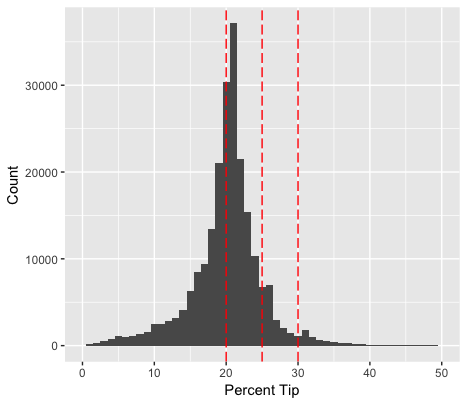
\includegraphics[width=3.89in]{figure/region_vis} 

}

\caption{Percent Tip Paid by Passengers in Each Pick-up and Drop-off Pair in NYC}\label{fig:region-vis}
\end{figure}
Figure \ref{fig:region-vis} is a histogram of mean tip percent for all
known pick-up and drop-off zone pairs. The red dash lines are drawn at
20\%, 25\%, and 30\%, which are the default percentage of tips that are
shown on the touch panel for credit and debit car payments (see Figure
\ref{fig:taxi-screen}), and passengers tend to pick the lowest default
percent tip.
\begin{figure}[h]

{\centering 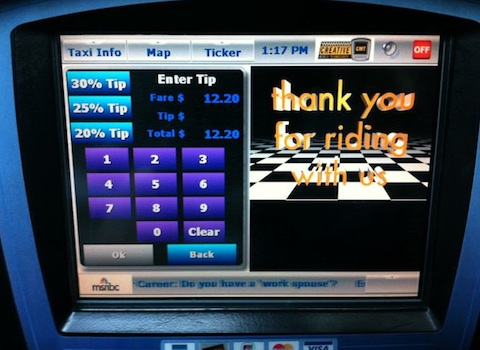
\includegraphics[width=4.8in]{figure/taxi-screen} 

}

\caption{Tip Payment Page on New York City Touch Panel}\label{fig:taxi-screen}
\end{figure}
\subsection{Pick-up Zone Percent Tips
Amount}\label{pick-up-zone-percent-tips-amount}

Taxi drivers are required to be indifferent to where passengers are
going. It is illegal for New York city taxi drivers to refuse service
because of passengers' race, ethnicity, cultural background, disability,
gender, or destination (N. T. Staff, 2018). Taxi drivers cannot choose
where the passengers want to go, and instead they can only choose which
pick-up zone they would prefer to drive around to get hailed. Therefore,
it makes sense to investigate the average amount of tips paid by
passengers departed from each pick-up zone. What are the taxi pick-up
zone that have the highest percent tips paid by passengers?
\begin{table}

\caption{\label{tab:unnamed-chunk-39}Ten taxi pick-up zones with the highest average tip in January, 2017}
\centering
\begin{tabular}[t]{ccc}
\toprule
Borough & Zone & Average \% Tips\\
\midrule
Queens & Douglaston & 29\\
Bronx & East Tremont & 29\\
Queens & Oakland Gardens & 29\\
Queens & Glendale & 28\\
Queens & Saint Michaels Cemetery/Woodside & 28\\
\addlinespace
Queens & Bayside & 27\\
Brooklyn & Coney Island & 27\\
Queens & Howard Beach & 27\\
Brooklyn & Marine Park/Mill Basin & 27\\
Bronx & Norwood & 26\\
\bottomrule
\end{tabular}
\end{table}
We calculated the average percent tip paid for each pick-up zone as
shown in Table 3.1. According to Table 3.1, 6 out of 10 taxi zones with
the highest average percent tips are in Queens. At a first glance,
Queens seems to be a good place for taxi drivers to go and pick up
passengers to make more money.

\subsection{Which taxi zones are the most popular ones for
pick-ups?}\label{which-taxi-zones-are-the-most-popular-ones-for-pick-ups}

Which pick-up zones have the highest number of taxi trip pick-ups? We
can create a heat map to visualize the number of trips for each pick-up
zones on a map of New York City Taxi Zones.
\begin{figure}[h]

{\centering 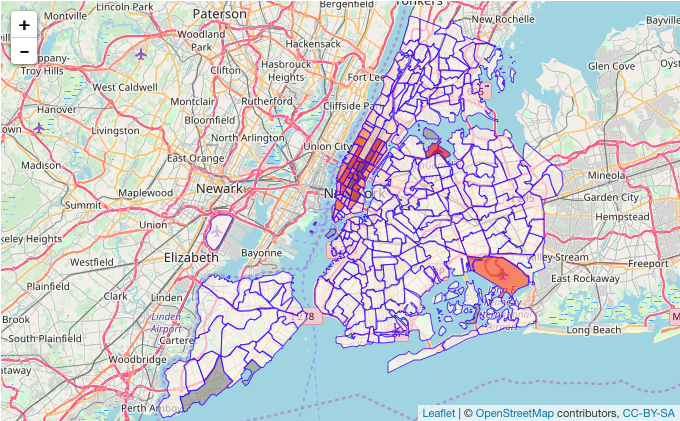
\includegraphics[width=5.84in]{figure/num_trip} 

}

\caption{Number of Pick-ups in Each Taxi Zone}\label{fig:num-trip}
\end{figure}
In Figure \ref{fig:num-trip}, taxi zones with more number of pick-ups
are colored by darker shades of orange, and it is obvious that Manhattan
and La Guardia Airport are the most popular locations for taxi pick-ups.
\begin{table}

\caption{\label{tab:unnamed-chunk-42}Ten taxi zones with the highest number of pick-ups}
\centering
\begin{tabular}[t]{ccc}
\toprule
Borough & Zone & Number of Trips\\
\midrule
Manhattan & Upper East Side South & 2519900\\
Manhattan & Midtown Center & 2461602\\
Manhattan & Union Sq & 2382970\\
Manhattan & Upper East Side North & 2372509\\
Manhattan & Midtown East & 2349386\\
\addlinespace
Manhattan & Murray Hill & 2231723\\
Manhattan & Penn Station/Madison Sq West & 2193036\\
Manhattan & East Village & 2097416\\
Queens & LaGuardia Airport & 2059444\\
Manhattan & Times Sq/Theatre District & 1972303\\
\bottomrule
\end{tabular}
\end{table}
Table 3.2 tells which specific taxi zones have the highest number of
pick-ups, and 9 out of the top 10 taxi zones that have the most number
of pick-ups are located in Manhattan. There are about 6000 yellow taxi
pick-ups in the top 10 taxi zones every day in 2017.

\subsection{Which pick-up zones have the highest percent
tips?}\label{which-pick-up-zones-have-the-highest-percent-tips}

Most yellow cab pick-ups occur in Manhattan. If we focus on the pick-up
zones that have at least 1 trip per hour (or 24 trips per day), we will
observe that many taxi pick-up zones with the highest percent tips are
not necessarily the ones with the highest number of pick-ups.
\begin{table}

\caption{\label{tab:unnamed-chunk-44}Ten taxi pick-up zones with the highest percent tip (taxi zones has at least 1 pick-up per hour)}
\centering
\begin{tabular}[t]{ccc}
\toprule
Borough & Zone & Average \% Tips\\
\midrule
Queens & Baisley Park & 21.55\\
Brooklyn & Gowanus & 21.45\\
Queens & Steinway & 21.36\\
Brooklyn & Carroll Gardens & 21.18\\
Queens & LaGuardia Airport & 21.00\\
\addlinespace
Brooklyn & Greenpoint & 21.00\\
Brooklyn & Prospect Heights & 21.00\\
Manhattan & Midtown Center & 20.82\\
Brooklyn & Cobble Hill & 20.82\\
Brooklyn & East Williamsburg & 20.82\\
\bottomrule
\end{tabular}
\end{table}
People might think it is more reasonable to see a list that is populated
with zones in Manhattan, since that's where most of the wealthy people
live. However, Table 3.3 shows that passengers who get on taxis from
certain zones in Brooklyn and Queens also pay a lot of tips. Taxi
drivers who would love to get higher percent tips can drive to the zones
listed above to pick-up passengers.

If we focus on the pick-up zones that have more than 1 trip per minute
(or 60 trips per hour), then we observe that all pick-up zones that have
the highest percent tips are in Manhattan besides La Guardia Airport.
\begin{table}

\caption{\label{tab:unnamed-chunk-46}Ten taxi pick-up zones with the highest percent tip (taxi zones has at least 1 pick-up per minute)}
\centering
\begin{tabular}[t]{ccc}
\toprule
Borough & Zone & Average \% Tips\\
\midrule
Queens & LaGuardia Airport & 21.00\\
Manhattan & Midtown Center & 20.82\\
Manhattan & Battery Park City & 20.73\\
Manhattan & Midtown East & 20.55\\
Manhattan & Murray Hill & 20.55\\
\addlinespace
Manhattan & Penn Station/Madison Sq West & 20.55\\
Manhattan & UN/Turtle Bay South & 20.45\\
Manhattan & Times Sq/Theatre District & 20.36\\
Manhattan & Union Sq & 20.18\\
Manhattan & Midtown North & 20.18\\
\bottomrule
\end{tabular}
\end{table}
There are more than 100 times more yellow cab pick-ups that happen in
Manhattan everyday than in Brooklyn. By comparing the average tip
percent in Table 3.3 and Table 3.4, we observe that 8 out of 10 average
percent tips in taxi zones with high pick-up numbers in Table 3.4 are
lower than average percent tips in taxi zones with low pick-up numbers
in Table 3.3. Therefore, there could be a correlation between number of
trips and average percent tips that passengers pay, and this can be
further studied with more taxi-zone-specific data, such as median
household income, provided.

\section{What features of taxi trips increase the percent tip amount
that passengers
pay?}\label{what-features-of-taxi-trips-increase-the-percent-tip-amount-that-passengers-pay}

So far, we have learned what pick-up zones offer the highest percent
tip. Now, we want to dig into the relationships between percent tip and
taxi-zone-specific variables.

\subsection{Does trip distance increase the percent tips paid by
passengers?}\label{does-trip-distance-increase-the-percent-tips-paid-by-passengers}

Do longer trips result in higher tip percent? It takes taxi drivers more
time to complete longer trips, so passengers might want to compensate
taxi drivers more.
\begin{Shaded}
\begin{Highlighting}[]
\NormalTok{tip_distance <-}\StringTok{ }\KeywordTok{lm}\NormalTok{(avg_tip }\OperatorTok{~}\StringTok{ }\NormalTok{avg_dis }\OperatorTok{+}\StringTok{ }\NormalTok{PULocationID }\OperatorTok{+}\StringTok{ }\NormalTok{DOLocationID, }\DataTypeTok{data =}\NormalTok{ tip_region)}
\end{Highlighting}
\end{Shaded}
\begin{verbatim}
                Estimate   Std. Error   t value Pr(>|t|)
(Intercept)  0.211325482 3.733048e-04 566.09360        0
avg_dis     -0.001052903 2.105014e-05 -50.01881        0
\end{verbatim}
According to the simple linear regression result, trip distance does
have a small negative impact on the percent of tips paid, controlling
for both pick-up and drop-off locations. Since the number of
observations in this regression model is big, the p-value quickly goes
to zero. Therefore, in this regression, p-value does not matter so much.
What is important in this result is the negative correlation between
average percent tips and average distance that a taxi travels.

The negative correlation could be caused by a psychological reason. Long
trips cost more than short trips. For a constant tip percent, the
nominal value of tip amount cost more for longer trips. For example, for
a \$100 trip, 20\% tip costs \$20; for a \$50 trip, 20\% tip costs \$10.
Even though consumers are paying the same percent of tips, \$20 is more
expensive than \$10. Therefore, consumers might decide to pay less
percent tip for longer trips.

\subsection{Do passengers pay more tips during rush
hours?}\label{do-passengers-pay-more-tips-during-rush-hours}

New York City Taxi Fare \& Limousine Commission has information on how
New York City taxi fare amount is calculated on their
\href{http://www.nyc.gov/html/tlc/html/passenger/taxicab_rate.shtml}{official
website}.

\subsubsection{Metered Fare Information}\label{metered-fare-information}
\begin{itemize}
\tightlist
\item
  Onscreen rate is `Rate \#01 -- Standard City Rate.'
\item
  The initial charge is \$2.50.
\item
  Plus 50 cents per 1/5 mile or 50 cents per 60 seconds in slow traffic
  or when the vehicle is stopped.
\item
  In moving traffic on Manhattan streets, the meter should ``click''
  approximately every four downtown blocks, or one block going
  cross-town (East-West).
\item
  There is a 50-cent MTA State Surcharge for all trips that end in New
  York City or Nassau, Suffolk, Westchester, Rockland, Dutchess, Orange
  or Putnam Counties.
\item
  There is a 30-cent Improvement Surcharge.
\item
  There is a daily 50-cent surcharge from 8pm to 6am.
\item
  There is a \$1 surcharge from 4pm to 8pm on weekdays, excluding
  holidays.
\item
  Passengers must pay all bridge and tunnel tolls.
\item
  Your receipt will show your total fare including tolls. Please take
  your receipt.
\item
  The driver is not required to accept bills over \$20.
\item
  Please tip your driver for safety and good service.
\item
  There are no charges for extra passengers or bags.
\end{itemize}
The metered fare rate information is collected from TLC rate of fare
webpage (N. T. Staff, 1996).

In taxi fare calculation, the only unknown variable is slow-traffic
time, and all other variables were collected by the meters installed on
each medallion taxi for each trip. It is reasonable to assume that for
trips with the same pick-up and drop-off locations, the longer the total
slow traffic time is, the longer the trip would take. Taxi drivers are
compensated for both the normal-speed trip distance and the time spent
in slow-traffic. According to the fare calculation algorithm, in moving
traffic on Manhattan streets, the meter should ``click'' approximately
every four downtown blocks, or one block going cross-town (East-West);
in slow traffic, the meter should ``click'' every 60 seconds. Therefore,
slow traffic increases the minute per mile ratio.

Does minute per mile ratio have an impact on the percent tip that
passengers pay? Do passengers compensate taxi drivers more during rush
hours? Are passengers sympathetic to taxi drivers for the time they
spend in slow traffic?
\begin{Shaded}
\begin{Highlighting}[]
\NormalTok{min_mile_ratio <-}\StringTok{ }\KeywordTok{lm}\NormalTok{(avg_tip }\OperatorTok{~}\StringTok{ }\NormalTok{min_per_mile, }\DataTypeTok{data =}\NormalTok{ yellow_2017_summary_small)}
\end{Highlighting}
\end{Shaded}
\begin{verbatim}
                Estimate   Std. Error   t value Pr(>|t|)
(Intercept)  0.193453599 1.870711e-04 1034.1180        0
min_per_mile 0.002841351 3.134322e-05   90.6528        0
\end{verbatim}
As shown in the regression result, \texttt{min\_per\_mile} ratio does
have a small positive impact on percent tips. Since trips with slow
traffic can be depicted by high minute per mile ratio, passengers do pay
more tips during rush hours.

\section{Recommendations to Taxi
Drivers}\label{recommendations-to-taxi-drivers}

Our analysis has suggested that taxi passengers are sympathetic with the
drivers who have to suffer the congestion in New York City, so we hope
that taxi drivers would feel better during rush hours by knowing that
passengers do pay for tips to compensate the negative feelings that
drivers carry in congestion.

\chapter{New York City Taxi Passengers}\label{chapter4}

\section{How long does it take passengers to get to JFK, La Guardia, and
Newark Airports from anywhere in New York
City?}\label{how-long-does-it-take-passengers-to-get-to-jfk-la-guardia-and-newark-airports-from-anywhere-in-new-york-city}

We want to calculate the average number of minutes it takes to go to all
three airports from a specific taxi zone at every hour. First, we want
to focus on trips going to any of the three airports, JFK, LaGuardia, or
Newark Airport. We need to load trip records with destination as one of
the three airports from the MySQL connection we built.
\begin{Shaded}
\begin{Highlighting}[]
\CommentTok{# extract data of trips going to JFK Airport}
\CommentTok{# from MySQL database}
\NormalTok{to_jfk_trip <-}\StringTok{ }\NormalTok{taxi }\OperatorTok
\StringTok{  }\KeywordTok{tbl}\NormalTok{(}\StringTok{"yellow"}\NormalTok{) }\OperatorTok
\StringTok{  }\KeywordTok{filter}\NormalTok{(DOLocationID }\OperatorTok{==}\StringTok{ }\DecValTok{132}\NormalTok{) }

\CommentTok{# extract data of trips going to La Guardia Airport}
\CommentTok{# from MySQL database}
\NormalTok{to_lg_trip <-}\StringTok{ }\NormalTok{taxi }\OperatorTok
\StringTok{  }\KeywordTok{tbl}\NormalTok{(}\StringTok{"yellow"}\NormalTok{) }\OperatorTok
\StringTok{  }\KeywordTok{filter}\NormalTok{(DOLocationID }\OperatorTok{==}\StringTok{ }\DecValTok{138}\NormalTok{) }

\CommentTok{# extract data of trips going to Newark Airport}
\CommentTok{# from MySQL database}
\NormalTok{to_newark_trip <-}\StringTok{ }\NormalTok{taxi }\OperatorTok
\StringTok{  }\KeywordTok{tbl}\NormalTok{(}\StringTok{"yellow"}\NormalTok{) }\OperatorTok
\StringTok{  }\KeywordTok{filter}\NormalTok{(DOLocationID }\OperatorTok{==}\StringTok{ }\DecValTok{1}\NormalTok{) }
\end{Highlighting}
\end{Shaded}
Now we want to calculate the average amount of time it takes from each
zone to one of the three airports during each hour.

So far, we have created three tables summarizing the average number of
minutes it takes to go to all three airports for every hour from
different taxi zones. It would be easier if we combine all three tables
and put information related to trip duration to all three airports in
the same table.
\begin{table}

\caption{\label{tab:unnamed-chunk-59}Average number of minutes it takes from Alphabet City, Manhattan to JFK Airport during different hours}
\centering
\begin{tabular}[t]{lcccc}
\toprule
  & Borough & Zone & Hour of Departure & Average Number of Minutes\\
\midrule
10 & Manhattan & Alphabet City & 0 & 45.37000\\
11 & Manhattan & Alphabet City & 1 & 36.77500\\
12 & Manhattan & Alphabet City & 2 & 28.66000\\
13 & Manhattan & Alphabet City & 3 & 27.83350\\
14 & Manhattan & Alphabet City & 4 & 27.19490\\
\addlinespace
15 & Manhattan & Alphabet City & 5 & 28.68889\\
16 & Manhattan & Alphabet City & 6 & 34.25271\\
17 & Manhattan & Alphabet City & 7 & 38.13817\\
18 & Manhattan & Alphabet City & 8 & 41.59687\\
19 & Manhattan & Alphabet City & 9 & 35.39226\\
\addlinespace
20 & Manhattan & Alphabet City & 10 & 36.22867\\
21 & Manhattan & Alphabet City & 11 & 41.12000\\
22 & Manhattan & Alphabet City & 12 & 41.02800\\
\bottomrule
\end{tabular}
\end{table}
Table 4.1 displays the average number of minutes it takes from Alphabet
City, Manhattan to JFK Airport during different hours.

\subsection{Case Study: From Central Park, Manhattan to all three
airports}\label{case-study-from-central-park-manhattan-to-all-three-airports}

Central Park, Manhattan has pick-up zone ID number 43. Let's take a look
at how much time is needed to travel to all three airports from taxi
zone No.4.
\begin{figure}[h]
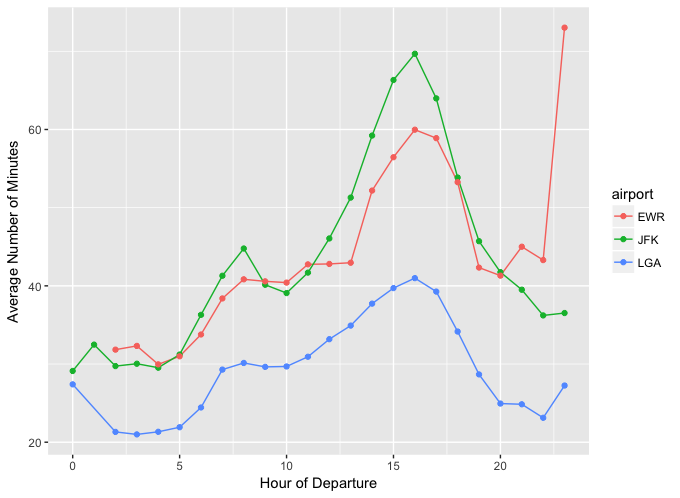
\includegraphics[width=5.67in]{figure/airport_vis} \caption{Average number of minutes it takes from Central Park, Manhattan to all three airports during different hours}\label{fig:airport-vis}
\end{figure}
According to the red line Figure \ref{fig:airport-vis}, it takes the
least time, less than 30 minutes, to travel from Central Park, Manhattan
to Newark Airport around 4 AM in the morning and it takes more than 70
minutes around 11 PM at night.

According to the green line, it only takes about 30 minutes to travel to
JFK Airport around 4 AM in the morning, and it takes the most time,
about 70 minutes, around 4 PM in the afternoon.

As shown by the blue line, it takes the least time, about 20 minutes, to
travel to La Guardia Airport at 2 AM at midnight, and it takes a little
more than 40 minutes around 4 PM in the evening.

Being able to know the average time it takes to go to one of the
airports ahead, passengers can buy their flight tickets accordingly. For
example, a mum who wants to visit Disney World with her kids can use
this visualization to estimate the amount of time needed for her and her
families to catch their flight. If this mum wants to catch a flight that
departs at 10 AM from JFK Airport, then when she should depart from
Central Park in order to get to the airport on time? According to Figure
\ref{fig:airport-vis}, she can depart at 7 AM, and it will take about 40
minutes for her to get to JFK Airport to catch her 10 AM flight.

\subsection{A Shiny App: When is the best time to travel to JFK
Airport?}\label{a-shiny-app-when-is-the-best-time-to-travel-to-jfk-airport}
\begin{center}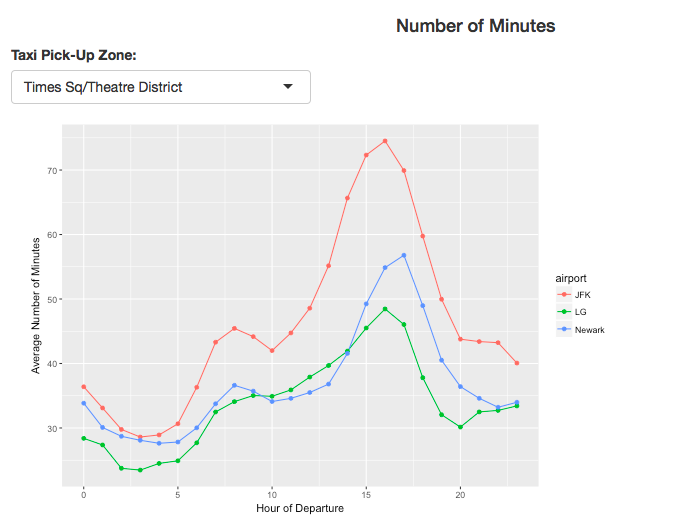
\includegraphics[width=6.74in]{figure/shinyapp} \end{center}

According to \ref{fig:shinyapp}, a person travelling from Times Square
to JFK Airport to catch a 11AM flight need to depart around 8:30 AM in
order to arrive at the airport 2 hours before the flight departs.

This Shiny App helps passengers to estimate the amount of time that is
needed for them to travel to any one of the three airports from any New
York City taxi zones.

\section{How does weather affect the number of taxi and Uber
trips?}\label{how-does-weather-affect-the-number-of-taxi-and-uber-trips}

On a snowy or rainy day, it is hard for passengers to find a yellow cab
on the street. Taxi drivers get paid at the same rate no matter how bad
the weather gets, so they tend to stay at home instead of going out to
work when the weather is bad. Uber drivers, however, get paid more on a
snowy or rainy day, since Uber uses a pricing model that takes supply
and demand into account. When weather is bad, demand for rides is
higher, so Uber fare rate increases. Uber's pricing model gives Uber
drivers an incentive to work extra hard on ugly days.

In this section, we study the number of pickups of yellow cab and Uber.
We compare number of pick-ups in each taxi zone in the weeks of bad
weather with previous weeks' total number of pick-ups to see whether
Uber drivers have an incentive to drive around the city more when
weather gets bad.

\textbf{Uber Weekly Data} We first calculated the number of total
dispatched trips of Uber by using weekly-aggregated Uber pick-up data
available on NYC OpenData (N. O. Staff, 2015b), and summary is shown in
Table 4.2.
\begin{table}

\caption{\label{tab:unnamed-chunk-65}Uber 2017 Weekly Total Dispatched Trips}
\centering
\begin{tabular}[t]{ccc}
\toprule
Pickup Start Date & Pickup End Date & Uber Total Dispatched Trips\\
\midrule
2017-01-01 & 2017-01-07 & 2866569\\
2017-01-08 & 2017-01-14 & 3114792\\
2017-01-15 & 2017-01-21 & 3089595\\
2017-01-22 & 2017-01-28 & 3299763\\
2017-01-29 & 2017-02-04 & 3224451\\
\addlinespace
2017-02-05 & 2017-02-11 & 3310481\\
2017-02-12 & 2017-02-18 & 3456042\\
2017-02-19 & 2017-02-25 & 3194805\\
2017-02-26 & 2017-03-04 & 3533347\\
2017-03-05 & 2017-03-11 & 3614559\\
\bottomrule
\end{tabular}
\end{table}
\subsubsection{Yellow Cab Weekly Data}\label{yellow-cab-weekly-data}

We also calculated the number of total dispatched trips of New York City
yellow cabs by using \texttt{nyctaxi} package to retrieve yellow taxi
data from 2017, and the summary is shown in Table 4.3.
\begin{table}

\caption{\label{tab:unnamed-chunk-68}Yellow Taxi 2017 Weekly Total Dispatched Trips}
\centering
\begin{tabular}[t]{ccc}
\toprule
Pickup Start Date & Pickup End Date & Yellow Total Dispatched Trips\\
\midrule
2017-01-01 & 2017-01-07 & 2044643\\
2017-01-08 & 2017-01-14 & 2230950\\
2017-01-15 & 2017-01-21 & 2219214\\
2017-01-22 & 2017-01-28 & 2307122\\
2017-01-29 & 2017-02-04 & 2331749\\
\addlinespace
2017-02-05 & 2017-02-11 & 2181622\\
2017-02-12 & 2017-02-18 & 2387399\\
2017-02-19 & 2017-02-25 & 2225850\\
2017-02-26 & 2017-03-04 & 2464800\\
2017-03-05 & 2017-03-11 & 2456285\\
\bottomrule
\end{tabular}
\end{table}
\subsection{Case Study: March 14th, 2017 Snow
Storm}\label{case-study-march-14th-2017-snow-storm}

On March 14th, 2017, a snow storm brought seven inches of snow to New
York City.

\textbf{Yellow Taxi}
\begin{table}

\caption{\label{tab:unnamed-chunk-70}Yellow Taxi Total Dispatched Trips}
\centering
\begin{tabular}[t]{ccc}
\toprule
Pickup Start Date & Pickup End Date & Yellow Total Dispatched Trips\\
\midrule
2017-03-05 & 2017-03-11 & 2456285\\
2017-03-12 & 2017-03-18 & 2066285\\
\bottomrule
\end{tabular}
\end{table}
\begin{Shaded}
\begin{Highlighting}[]
\NormalTok{(}\DecValTok{2066285}\OperatorTok{-}\DecValTok{2456285}\NormalTok{)}\OperatorTok{/}\DecValTok{2456285}
\end{Highlighting}
\end{Shaded}
\begin{verbatim}
[1] -0.1587764
\end{verbatim}
Yellow taxi's number of total dispatched trips declined by 15\% (see
Table 4.4).

\textbf{Uber}
\begin{table}

\caption{\label{tab:unnamed-chunk-73}Uber Total Dispatched Trips}
\centering
\begin{tabular}[t]{ccc}
\toprule
Pickup Start Date & Pickup End Date & Uber Total Dispatched Trips\\
\midrule
2017-03-05 & 2017-03-11 & 3614559\\
2017-03-12 & 2017-03-18 & 3430189\\
\bottomrule
\end{tabular}
\end{table}
\begin{Shaded}
\begin{Highlighting}[]
\NormalTok{(}\DecValTok{3430189}\OperatorTok{-}\DecValTok{3614559}\NormalTok{)}\OperatorTok{/}\DecValTok{3614559}
\end{Highlighting}
\end{Shaded}
\begin{verbatim}
[1] -0.05100761
\end{verbatim}
Uber's number of total dispatched trips declined by 5\% (see Table 4.5).

In this case, we observe that the percent decline in Uber's total number
of pick-ups is 10\% less than the percent decline in Yellow Taxi's total
number of drop-off. Even though the total number of Uber pick-ups did
not increase, Uber's pricing model may keep more drivers in the market
on a snowy day.

\subsection{Case Study: Impact of Precipitation on Taxi
Rides}\label{case-study-impact-of-precipitation-on-taxi-rides}

People living in New York might have noticed that it is hard to find a
taxi on the street when it rains. Economists have studied this phenomena
for a long time, and an analysis that studied the correlation between
taxi movement and hourly rainfall data in Central Park from 2009 to 2013
found that there is no significant correlation between a driver's hourly
wage and precipitation in the city, which implies that drivers don't
earn more or less when it rains (Jaffe, 2014).

We got access to the 2017 daily Central Park weather data from the
National Climatic Data Center by submitting a Climate Data Online
request (Appendix D) to National Centers for Environmental Information
(Environmental Information Staff, 2018), and joined it to the 2017 taxi
data to study relationship between rainfall and taxi rides.

First, we generate a list of total amount of daily rainfall in New York
City and we pick the 10 weeks that have the most rainfall in 2017 (see
Table 4.6).
\begin{table}

\caption{\label{tab:unnamed-chunk-76}10 weeks that have the most rainfall in 2017}
\centering
\begin{tabular}[t]{ccc}
\toprule
Pickup Start Date & Pickup End Date & Weekly Rainfall\\
\midrule
2017-06-18 & 2017-06-25 & 7.00\\
2017-04-30 & 2017-05-07 & 6.71\\
2017-10-29 & 2017-11-05 & 6.16\\
2017-07-02 & 2017-07-09 & 5.56\\
2017-03-26 & 2017-04-02 & 5.11\\
\addlinespace
2017-01-22 & 2017-01-29 & 3.99\\
2017-08-13 & 2017-08-20 & 3.95\\
2017-06-11 & 2017-06-18 & 3.91\\
2017-04-02 & 2017-04-09 & 3.17\\
2017-04-23 & 2017-04-30 & 2.88\\
\bottomrule
\end{tabular}
\end{table}
We then find the weekly total number of dispatched yellow taxi trips of
the 10 weeks with the most rainfall (see Table 4.7).
\begin{table}

\caption{\label{tab:unnamed-chunk-78}10 weeks that have the most rainfall in 2017 and the total number of dispatched yellow taxi trips in those weeks}
\centering
\begin{tabular}[t]{ccccc}
\toprule
Pickup Date & Dispatched Trips & Last Week Date & Last Week Trips & \% Change Trips\\
\midrule
2017-06-18 & 2231205 & 2017-06-11 & 2285958 & -2.40\\
2017-04-30 & 2386559 & 2017-04-23 & 2394329 & -0.32\\
2017-10-29 & 2266196 & 2017-10-22 & 2267693 & -0.07\\
2017-07-02 & 1664159 & 2017-06-25 & 2038406 & -18.36\\
2017-03-26 & 2341096 & 2017-03-19 & 2272369 & 3.02\\
\addlinespace
2017-01-22 & 2307122 & 2017-01-15 & 2219214 & 3.96\\
2017-08-13 & 1871668 & 2017-08-06 & 1929860 & -3.02\\
2017-06-11 & 2285958 & 2017-06-04 & 2313236 & -1.18\\
2017-04-02 & 2414700 & 2017-03-26 & 2341096 & 3.14\\
2017-04-23 & 2394329 & 2017-04-16 & 2337161 & 2.45\\
\bottomrule
\end{tabular}
\end{table}
We also need to add the weekly total number of dispatched Uber trips of
the 10 weeks with the most rainfall (see Table 4.8).
\begin{table}

\caption{\label{tab:unnamed-chunk-80}10 weeks that have the most rainfall in 2017 and the total number of dispatched Uber trips in those weeks}
\centering
\begin{tabular}[t]{ccccc}
\toprule
Pickup Date & Dispatched Trips & Last Week Date & Last Week Trips & \% Change Trips\\
\midrule
2017-06-18 & 3654932 & 2017-06-11 & 3658220 & -0.09\\
2017-04-30 & 3546893 & 2017-04-23 & 3606408 & -1.65\\
2017-10-29 & 4317572 & 2017-10-22 & 4193611 & 2.96\\
2017-07-02 & 3212582 & 2017-06-25 & 3406814 & -5.70\\
2017-03-26 & 3541624 & 2017-03-19 & 3425475 & 3.39\\
\addlinespace
2017-01-22 & 3299763 & 2017-01-15 & 3089595 & 6.80\\
2017-08-13 & 3599772 & 2017-08-06 & 3584023 & 0.44\\
2017-06-11 & 3658220 & 2017-06-04 & 3622252 & 0.99\\
2017-04-02 & 3443444 & 2017-03-26 & 3541624 & -2.77\\
2017-04-23 & 3606408 & 2017-04-16 & 3427564 & 5.22\\
\bottomrule
\end{tabular}
\end{table}
We combine the percentage change in total number of dispatched trips of
yellow taxi and Uber, and we compare the result (see Table 4.9).
\begin{table}

\caption{\label{tab:unnamed-chunk-82}The percentage change in total number of dispatched trips comparing to the previous weeks of yellow taxi and Uber}
\centering
\begin{tabular}[t]{ccccc}
\toprule
Pickup Start Date & Weekly Rainfall & Last Week Date & Uber & Yellow\\
\midrule
2017-06-18 & 7.00 & 2017-06-11 & -0.09 & -2.40\\
2017-04-30 & 6.71 & 2017-04-23 & -1.65 & -0.32\\
2017-10-29 & 6.16 & 2017-10-22 & 2.96 & -0.07\\
2017-07-02 & 5.56 & 2017-06-25 & -5.70 & -18.36\\
2017-03-26 & 5.11 & 2017-03-19 & 3.39 & 3.02\\
\addlinespace
2017-01-22 & 3.99 & 2017-01-15 & 6.80 & 3.96\\
2017-08-13 & 3.95 & 2017-08-06 & 0.44 & -3.02\\
2017-06-11 & 3.91 & 2017-06-04 & 0.99 & -1.18\\
2017-04-02 & 3.17 & 2017-03-26 & -2.77 & 3.14\\
2017-04-23 & 2.88 & 2017-04-16 & 5.22 & 2.45\\
\bottomrule
\end{tabular}
\end{table}
Besides the week of April 30th, 2017, all other weeks have higher
increases in the number of total dispatched trips of Uber or lower
declines in the number of weekly Uber trips. Therefore, on rainy days,
Uber drivers tend to increase the number of trips they drive at a higher
rate.

We then plot the weekly rainfall and Yellow Taxi and Uber's percent
Change in Number of Dispatched Trips from Previous Week.
\begin{center}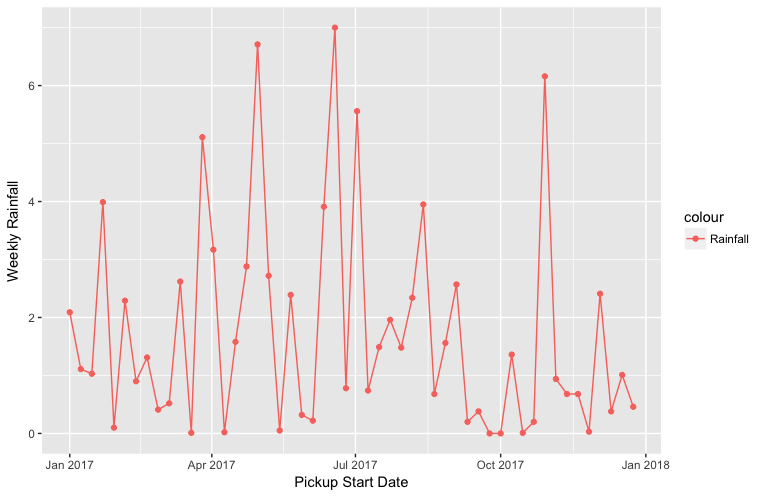
\includegraphics[width=6.37in]{figure/rainfall_vis} \end{center}
\begin{center}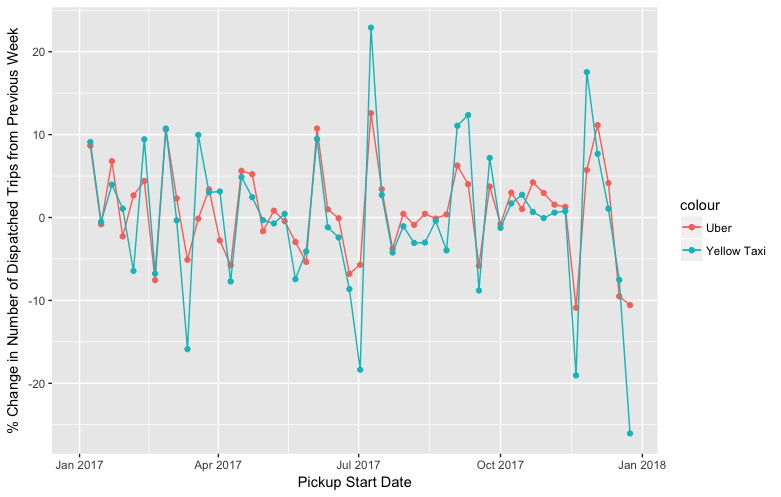
\includegraphics[width=6.51in]{figure/weather_vis} \end{center}

According to Figure @ref(fig:rainfall\_vis) and Figure
@ref(fig:weather\_vis), when weekly rainfall is high, Uber usually have
less percent decline in total number of dispatched trips comparing to
the total number of trips from previous week than yellow cab does. Uber
passengers pay higher fare on rainy days because of Uber's pricing
model. Since taxi drivers do not get paid more on rainy days, they tend
to work less than Uber drivers, which limits the options for passengers.
Passengers sometimes have to choose the more expensive Uber instead
(Jaffe, 2014).

\section{Recommendations to Taxi
Passengers}\label{recommendations-to-taxi-passengers}

We suggest passengers to use our Shiny App to choose a pick-up zone of
their interest and then decide when is the most favorable time for them
to travel from that zone to any of the three airports in New York.

\chapter{New York City Taxi \& Limousine Commission}\label{chapter5}

\section{Should there be a flat rate between Manhattan and John F.
Kennedy International
Airport?}\label{should-there-be-a-flat-rate-between-manhattan-and-john-f.-kennedy-international-airport}

Why is there a flat rate to and from JFK airport and any location in
Manhattan? Why is the flat rate \$52? Does TLC make profit from the \$52
flat rate? Does \$52 reduce the congestion on the road to JFK airport
and make taking a train a more preferable choice? The New York City taxi
trip records can reveal the answers to these questions.

Imagine it's your first time travelling to New York City, and you
decided to stay in a hotel in Manhattan. Since you might not know much
about the city, the fixed \$52 flat rate provides cost certainty for
you, and it incentivizes you to take taxi to JFK Airport. If there is no
flat rate, there is uncertainty in how much someone needs to pay to take
a taxi to JFK, and tourists might instead choose to take the train, even
though taking a train would cost them more time, anxiety, and
inconvenience.

Additionally, people living in most parts of Manhattan would have paid
more than \$52 to take a taxi to go to the JFK Airport. The higher the
taxi fare is, the less the demand for taxi will be. Therefore, having a
flat rate might help taxi drivers to get more trips from Manhattan to
JFK Airport.

\section{Passengers departing from Manhattan benefit from the \$52 flat
rate}\label{passengers-departing-from-manhattan-benefit-from-the-52-flat-rate}

If there is no flat rate between JFK and Manhattan, how much would
passengers pay for the distance they travelled between JFK Airport AND
Manhattan? And how much more or less should they have paid comparing to
the \$52 flat rate?

In this study, we are only interested in yellow taxi trip between
Manhattan and JFK Airport. Since JFK Airport's Location ID is 132, we
only retrieve trip records with either pick-up or drop-off location ID
as 132 from the database.
\begin{Shaded}
\begin{Highlighting}[]
\CommentTok{# extract yellow records of trips going to JFK Airport}
\CommentTok{# from a SQL database}
\NormalTok{to_jfk <-}\StringTok{ }\NormalTok{taxi }\OperatorTok
\StringTok{  }\KeywordTok{tbl}\NormalTok{(}\StringTok{"yellow"}\NormalTok{) }\OperatorTok
\StringTok{  }\KeywordTok{filter}\NormalTok{(DOLocationID }\OperatorTok{==}\StringTok{ }\DecValTok{132}\NormalTok{)}

\CommentTok{# extract yellow records of trips coming from JFK Airport}
\CommentTok{# from a SQL database}
\NormalTok{from_jfk <-}\StringTok{ }\NormalTok{taxi }\OperatorTok
\StringTok{  }\KeywordTok{tbl}\NormalTok{(}\StringTok{"yellow"}\NormalTok{) }\OperatorTok
\StringTok{  }\KeywordTok{filter}\NormalTok{(PULocationID }\OperatorTok{==}\StringTok{ }\DecValTok{132}\NormalTok{)}
\end{Highlighting}
\end{Shaded}
\subsection{Trips from Manhattan to JFK
Airport}\label{trips-from-manhattan-to-jfk-airport}

We first focus on all the trips that departed from Manhattan and went to
JFK Airport, and then we calculate the estimated taxi fare amount that
the passengers should have paid based on the distance travelled from
each pick-up point to JFK Airport based on the fare rate suggested by
TLC for each pick-up zone.
\begin{figure}[h]

{\centering 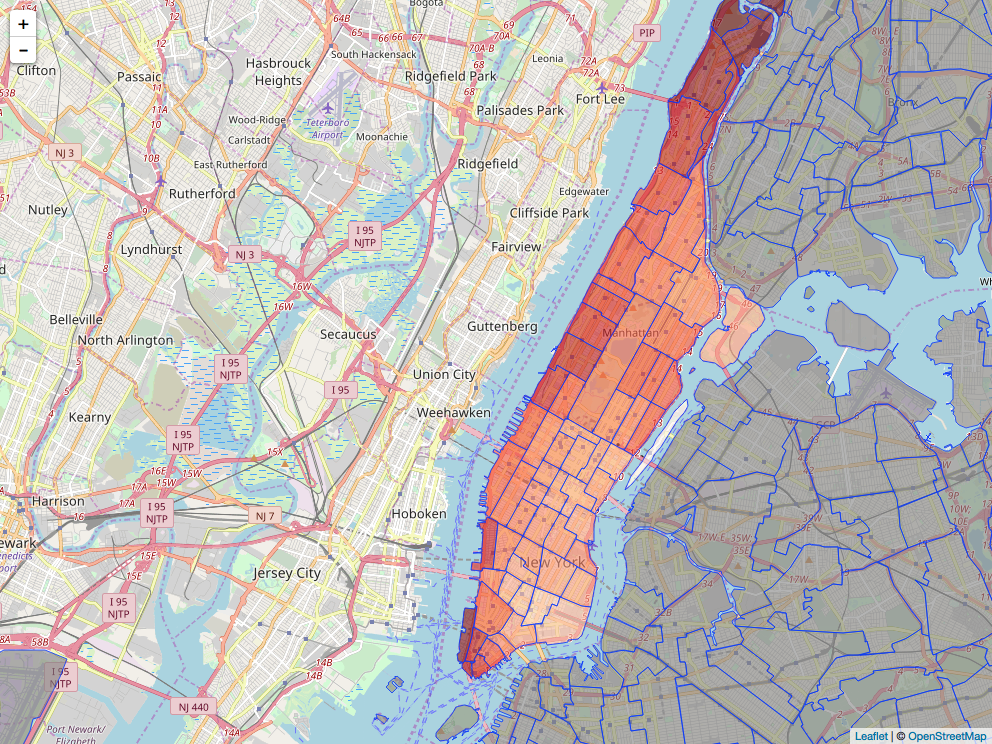
\includegraphics[width=5.84in]{figure/to_jfk_fare_vis} 

}

\caption{Estimated fare amount from each pick-up zone to JFK Airport}\label{fig:to-jfk-fare-vis}
\end{figure}
Figure \ref{fig:to-jfk-fare-vis} is a map of estimated fare amount
calculated by taking the average of all estimated fare amounts from the
same pick-up zone to JFK Airport based on the fare rate suggested by TLC
for each pick-up zone. According to the map, trips from Midtown on
average cost less than trips from other taxi zones in Manhattan.

\subsection{Which taxi zones would pay more than \$52 without the flat
rate?}\label{which-taxi-zones-would-pay-more-than-52-without-the-flat-rate}
\begin{table}

\caption{\label{tab:unnamed-chunk-95}Ten pick-up zones with the highest average  fare from Manhattan to JFK Airport}
\centering
\begin{tabular}[t]{cccc}
\toprule
avg\_est\_fare & avg\_est\_diff & Borough & Zone\\
\midrule
64.03150 & 11.844558 & Manhattan & Battery Park City\\
63.98256 & 9.970366 & Manhattan & Inwood\\
62.97567 & 10.892992 & Manhattan & Washington Heights North\\
61.99327 & 9.889636 & Manhattan & Battery Park\\
60.49388 & 8.278941 & Manhattan & Washington Heights South\\
\addlinespace
60.18006 & 8.107309 & Manhattan & Upper West Side South\\
59.74384 & 7.511991 & Manhattan & World Trade Center\\
59.31411 & 7.058534 & Manhattan & Meatpacking/West Village West\\
59.24692 & 7.200516 & Manhattan & Lincoln Square West\\
59.13439 & 7.083517 & Manhattan & Upper West Side North\\
\bottomrule
\end{tabular}
\end{table}
We computed the average fare paid by passengers for trips going from
each taxi zone in Manhattan to JFK Airport in Table 5.1.

Let's visualize the taxi zones that would have cost more than the \$52
flat rate.
\begin{figure}[h]

{\centering 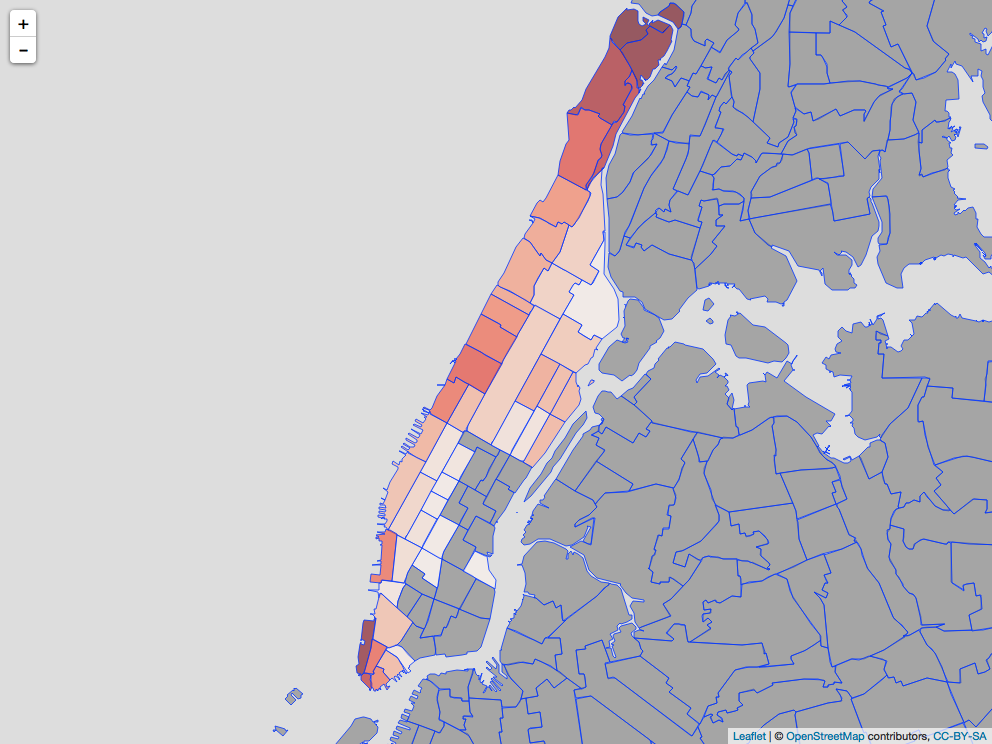
\includegraphics[width=5.84in]{figure/to_jfk_fare_above_vis} 

}

\caption{Pick-up Zones that cost more than the 52 US Dollar flat rate}\label{fig:to-jfk-fare-above-vis}
\end{figure}
Therefore, passengers from places in Manhattan besides Midtown, East
Village, and some parts of Lower Manhattan benefit from the \$52 flat
rate. However, people living in Midtown, East Village, and some parts of
Lower Manhattan might be relatively more indifferent to the price of
taxi, since they would pay less than \$52 without the flat rate.
Instead, they probably put more emphasis on convenience and time.

On average people travel from Manhattan pay \$2.83 less with the \$52
flat rate policy. Therefore, passengers overall benefit from the \$52
flat rate policy.

\section{Are taxi drivers happy when a passenger wants to go to JFK
Airport from
Manhattan?}\label{are-taxi-drivers-happy-when-a-passenger-wants-to-go-to-jfk-airport-from-manhattan}

Are taxi drivers happy when their passengers want to go to JFK Airport
from Manhattan? In this section, we study the hourly wage of taxi
drivers for different trips they completed, and we investigate whether
taxi driver hourly wage from Manhattan to JFK Airport is higher than
other trips.
\begin{verbatim}
[1] 63.29
\end{verbatim}
The average hourly wage of taxi drivers calculated by using all trips
excluding the ones going from Manhattan to JFK Airport is \$63.29.
\begin{verbatim}
[1] 69.05
\end{verbatim}
The average hourly wage of taxi drivers calculated by using trips going
from Manhattan to JFK Airport is \$69.05, slightly higher than \$63.29
dollar per hour, which means that on average taxi drivers driving from
Manhattan to JFK Airport have an hourly wage that is about \$6 higher
than the hourly wage of taxi drivers doing other trips.

\subsection{How much on average would taxi driver make on their way back
from JFK
Airport?}\label{how-much-on-average-would-taxi-driver-make-on-their-way-back-from-jfk-airport}

A taxi driver waiting in line to pick-up passengers at JFK Airport could
be directed back to anywhere in the city. Therefore, the estimated fare
that a taxi driver would make on the way back from JFK is unknown. We
calculate the average taxi fare amount that a taxi driver would get paid
for a trip from JFK Airport to any part of the city.

\subsubsection{What are the most popular drop-off locations for
passengers departing from JFK
Airport?}\label{what-are-the-most-popular-drop-off-locations-for-passengers-departing-from-jfk-airport}
\begin{table}

\caption{\label{tab:unnamed-chunk-102}5 most popular destinations in Manhattan}
\centering
\begin{tabular}[t]{ccccc}
\toprule
Borough & Zone & num\_trips & avg\_fare & avg\_duration\\
\midrule
Manhattan & Times Sq/Theatre District & 59419 & 69.80599 & 55.92389\\
Manhattan & Midtown East & 40513 & 69.40195 & 47.42096\\
Manhattan & Murray Hill & 40071 & 69.91174 & 43.66998\\
Manhattan & Midtown South & 38890 & 70.11065 & 48.34342\\
Manhattan & Midtown Center & 36405 & 69.64272 & 52.62410\\
\bottomrule
\end{tabular}
\end{table}
Table 5.2 shows that Times Square is the most popular destination for
passengers coming from the JFK Airport in 2017.
\begin{figure}[h]

{\centering 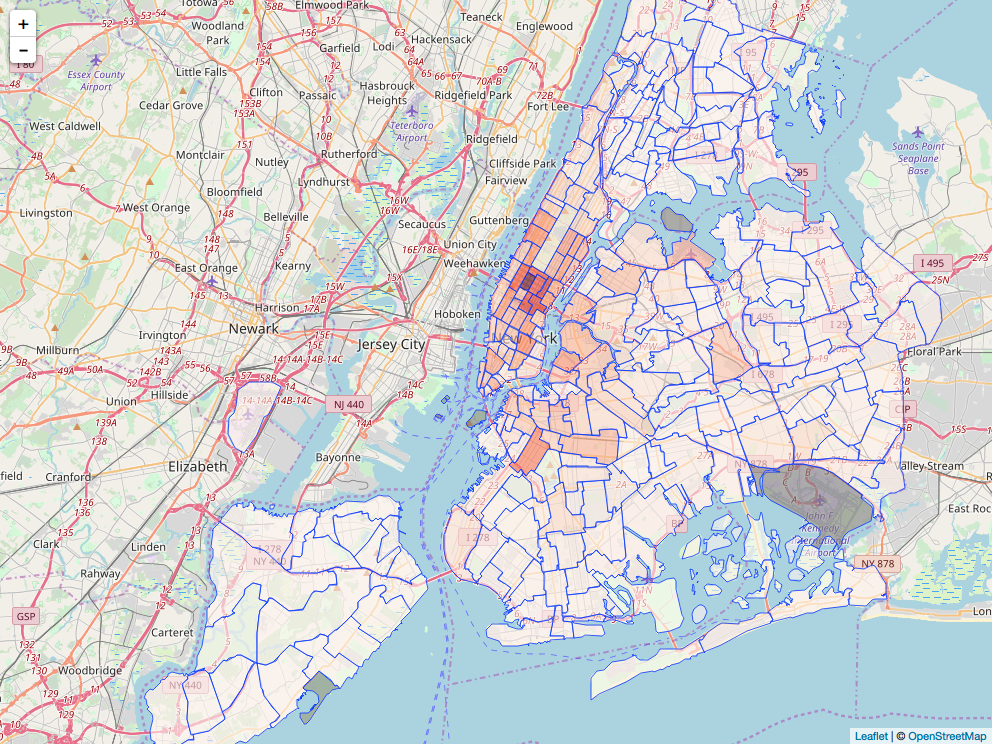
\includegraphics[width=5.84in]{figure/from_jfk_num_trips} 

}

\caption{Number of trips from JFK Airport to any Taxi Zones}\label{fig:from-jfk-num-trips}
\end{figure}
According to the Figure 5.3, Manhattan is the most popular destination
for passengers departing from JFK Airport.
\begin{table}

\caption{\label{tab:unnamed-chunk-105}Number of Trips going to Manhattan or other boroughs from JFK Airport}
\centering
\begin{tabular}[t]{cc}
\toprule
Going to Manhattan & Number of Trips\\
\midrule
0 & 521476\\
1 & 970366\\
\bottomrule
\end{tabular}
\end{table}
According to the summary, the total number of trips from JFK Airport to
Manhattan is about 65.04\% of the total number of trips travelling from
JFK Airport to all other Borough. Therefore, it is very likely for taxi
drivers to get passengers who want to go to Manhattan with a flat rate
of \$52.

\subsubsection{What's the average fare to each drop-off zone from JFK
Airport?}\label{whats-the-average-fare-to-each-drop-off-zone-from-jfk-airport}

We can use a map to visualize the distribution of average fare amount
needed to travel from JFK Airport to any taxi zone in New York City.
\begin{table}

\caption{\label{tab:unnamed-chunk-107}10 most popular taxi drop-off zones from JFK Airport with the corresponding average fare amount}
\centering
\begin{tabular}[t]{ccccc}
\toprule
Borough & Zone & \# of Trips & Average Fare & Average Duration\\
\midrule
Manhattan & Times Sq/Theatre District & 59419 & 69.81 & 55.92389\\
Manhattan & Midtown East & 40513 & 69.40 & 47.42096\\
Manhattan & Murray Hill & 40071 & 69.91 & 43.66998\\
Manhattan & Midtown South & 38890 & 70.11 & 48.34342\\
Manhattan & Midtown Center & 36405 & 69.64 & 52.62410\\
\addlinespace
Manhattan & Clinton East & 35297 & 69.20 & 55.78806\\
Manhattan & Midtown North & 34538 & 68.30 & 55.80455\\
Brooklyn & Park Slope & 27219 & 60.96 & 45.75234\\
Manhattan & East Village & 26595 & 66.98 & 45.45684\\
Manhattan & Upper West Side South & 24723 & 69.95 & 50.87777\\
\bottomrule
\end{tabular}
\end{table}
\begin{figure}[h]

{\centering 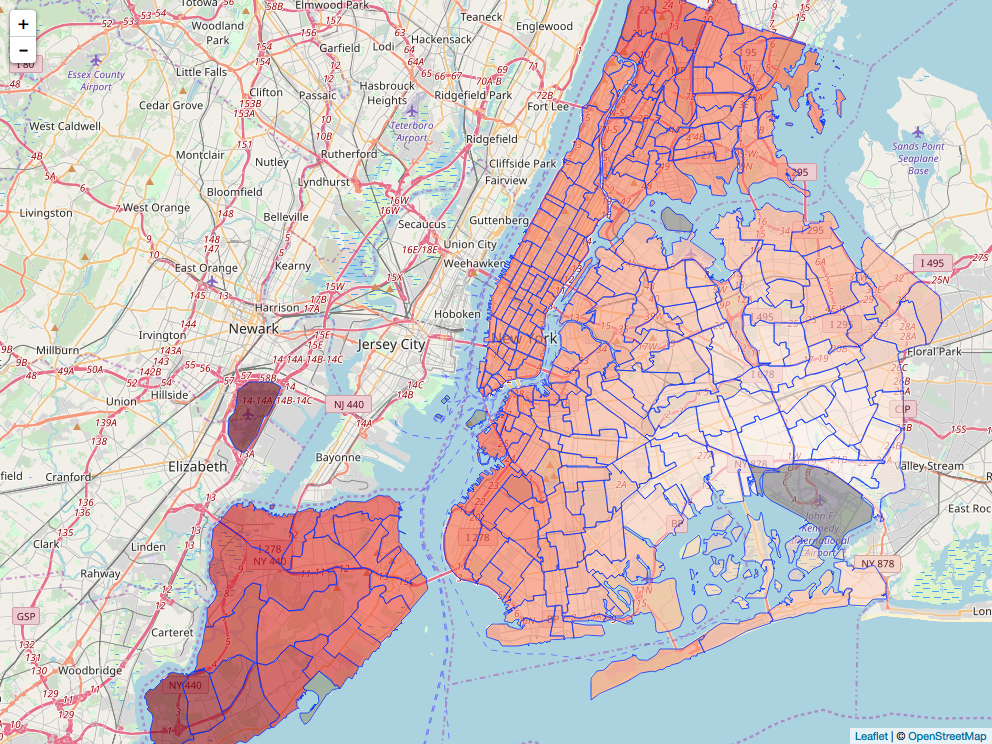
\includegraphics[width=5.84in]{figure/from_jfk_fare_vis} 

}

\caption{Zones that cost more than the 52 US Dollar flat rate}\label{fig:from-jfk-fare-vis}
\end{figure}
As we expected, the red shades are smoothly distributed, since taxi
zones that are futher away should cost more to get there.

\subsubsection{How much on average would taxi driver make on their way
back from JFK
Airport?}\label{how-much-on-average-would-taxi-driver-make-on-their-way-back-from-jfk-airport-1}
\begin{verbatim}
[1] 62.7
\end{verbatim}
On average, taxi drivers would get paid for on average \$62.7 for a trip
from the JFK Airport to any taxi zone in New York City, and on average
trips from JFK Airport last 44 minutes.
\begin{verbatim}
[1] 63.15
\end{verbatim}
The average hourly wage of taxi drivers calculated by using all trips
excluding the ones departing from JFK Airport is 63.15 dollar per hour.
\begin{verbatim}
[1] 94.65
\end{verbatim}
The average hourly wage of taxi drivers calculated by using trips
departing from JFK Airport is \$94.65 per hour, which means that on
average taxi drivers going from JFK Airport to any taxi zones in New
York City have an hourly wage that is more than \$30 higher than the
hourly wage of taxi drivers doing other trips.

\subsubsection{How much more do taxi drivers make on average for a round
trip to and from JFK Airport, comparing to any other
trips?}\label{how-much-more-do-taxi-drivers-make-on-average-for-a-round-trip-to-and-from-jfk-airport-comparing-to-any-other-trips}

On average taxi drivers driving from Manhattan to JFK Airport make \$6
more every hour than taxi drivers doing other trips. On average taxi
drivers going from JFK Airport to any taxi zones in New York City make
\$30 more every hour than taxi drivers doing other trips. Overall, a
taxi driver doing a round trip to and from JFK Airport make \$36 more
every hour, comparing to a taxi driver doing any other trips. In this
case, a round trip to and from JFK Airport is worthwhile, and that's why
taxi drivers should feel happy when pick up a passenger in Manhattan and
is told that he or she wants to go to JFK Airport.

\section{Recommendations to New York City Taxi Fare \& Limousine
Commission}\label{recommendations-to-new-york-city-taxi-fare-limousine-commission}

In this chapter, we have found the reason why taxicab drivers feel happy
when they pick up passengers who want to go to JFK Airport in Manhattan.
Even though \$52 is lower than the average amount of fare that taxi
drivers would have made without the flat rate, it still induces a higher
than average hourly wage, so it does not disincentive drivers to go to
JFK Airport from Manhattan. Therefore, we suggest the TLC to keep this
flat rate so that passengers do not have any uncertainty in cost and
they are more willing to take a taxi to travel to JFK Airport from
Manhattan.

\chapter{Conclusion}\label{chapter6}

In this Honors thesis, we present a more efficient and user-friendly way
for \textbf{R} users to retrieve trip record of both taxi and other
ride-sharing services, such as Uber and Lyft, in New York City.

By analyzing trip records of New York City's yellow taxi, we found
answers to questions that are of interest to taxi drivers, passengers,
and TLC officials:
\begin{itemize}
\item
  We found which taxi zones have passengers who offer the highest
  percent of tips, and we showed that taxi drivers do get compensated
  more during rush hours.
\item
  We helped passengers to know the average time it takes to go to one of
  the three airports in New York City so that passengers can plan their
  trips accordingly.
\item
  We also found that the \$52 flat rate between Manhattan and JFK
  Airport is beneficial for the passengers, because it is cheaper than
  the average amount of fare that passenger would need to pay without
  the flat rate.
\item
  We have also shown that the flat rate does not discourage drivers,
  even though taxi drivers would have been paid more without the flat
  rate.
\end{itemize}
We suggest passengers to use our Shiny App to choose a pick-up zone of
their interest and then decide when is the most favorable time for them
to travel to any airport in New York. We recommend New York City TLC to
modify the fare on rainy or snowy days to incentive taxicab drivers to
pick up more trips in order to make street-hail service more affordable
on rainy days for passengers. We also suggest the TLC to keep the \$52
flat rate between Manhattan and JFK Airport so that passengers do not
have any uncertainty in cost and they are more willing to take a taxi to
travel to JFK Airport from Manhattan.

\section{Future Research}\label{future-research}

With more time given, I would love to add more functionalities to
\texttt{nyctaxi} \textbf{R} package. I could include more types of
transportation in this package so that users not only can study
questions related to Uber or Lyft but also can investigate behaviors of
other e-hail services, such as Juno and Via. I could also include more
geographic locations in \texttt{nyctaxi} so that users can compare the
behaviors of multiple street-hail services across different cities.

Using \texttt{nyctaxi} \textbf{R} package, we can answer more
street-hail services related questions. We would love to investigate the
sharp decline in the consumption of NYC yellow cab after e-hail services
were introduced into the NYC ride-hail market (Board, 2018). By looking
into the patterns in market shares, it might be possible to predict the
future market share distribution and find out what features of
street-hail transportation are the ones that affect market share the
most.

As mentioned in Chapter 3, we also want to study the correlation between
number of trips and average percent tips in each taxi zone. If more
taxi-zone-specific data is provided, we could find out the true
correlation between the two variables.

We could also use \texttt{nyctaxi} \textbf{R} package to study the
impact of the newly-installed GPS and entertainment system in taxicabs
on the number of taxi rides. With the raised expectation among ride
experience caused by Uber and Lyft, yellow taxi industry need to respond
quickly (Hawkins, 2016). TLC decided to install GPS and entertainment
system in order to attract more passengers to take taxis. How does the
market react to the newly installed entertainment system? Has the market
share of yellow cab rebounded since the installation of the
entertainment system in 2016?

An article of The New York Times talks about the pros and cons of
introducing e-hail services into New York City. E-hail services are
beneficial to New Yorker who want to ``avoids their dysfunctional subway
system'', but they are turning New York City's already packed streets
into ``glorified parking lots'' (Board, 2018). With the help of
\texttt{nyctaxi} \textbf{R}, we want to further investigate the solution
of reducing traffic congestion in New York City by enforcing new
policies on e-hail services.

\appendix

\chapter{Utility Function}\label{utility-function}

This utility function was written to shorten the source code in ETL
\texttt{etl\_extract.etl\_nyctaxi()} function. It takes in
`\texttt{url}, \texttt{year}, \texttt{n} (number of observations), and
\texttt{names} (which are the names CSV data files), and create a list
of raw data directories.
\begin{Shaded}
\begin{Highlighting}[]
\NormalTok{download_nyc_data <-}\StringTok{ }\ControlFlowTok{function}\NormalTok{(obj, url, years, n, names, ...) \{}
\NormalTok{  url <-}\StringTok{ }\KeywordTok{paste0}\NormalTok{(url, }\StringTok{"?years="}\NormalTok{, years, }\StringTok{"&$limit="}\NormalTok{, n)}
\NormalTok{  lcl <-}\StringTok{ }\KeywordTok{file.path}\NormalTok{(}\KeywordTok{attr}\NormalTok{(obj, }\StringTok{"raw"}\NormalTok{), names)}
\NormalTok{  downloader}\OperatorTok{::}\KeywordTok{download}\NormalTok{(url, }\DataTypeTok{destfile =}\NormalTok{ lcl, ...)}
\NormalTok{  lcl}
\NormalTok{\}}
\end{Highlighting}
\end{Shaded}
\chapter{Data Dictionary -- Yellow
Taxi}\label{data-dictionary-yellow-taxi}

All variables used in data analysis of yellow taxi data are listed in
this data dictionary.
\begin{figure}[h]

{\centering 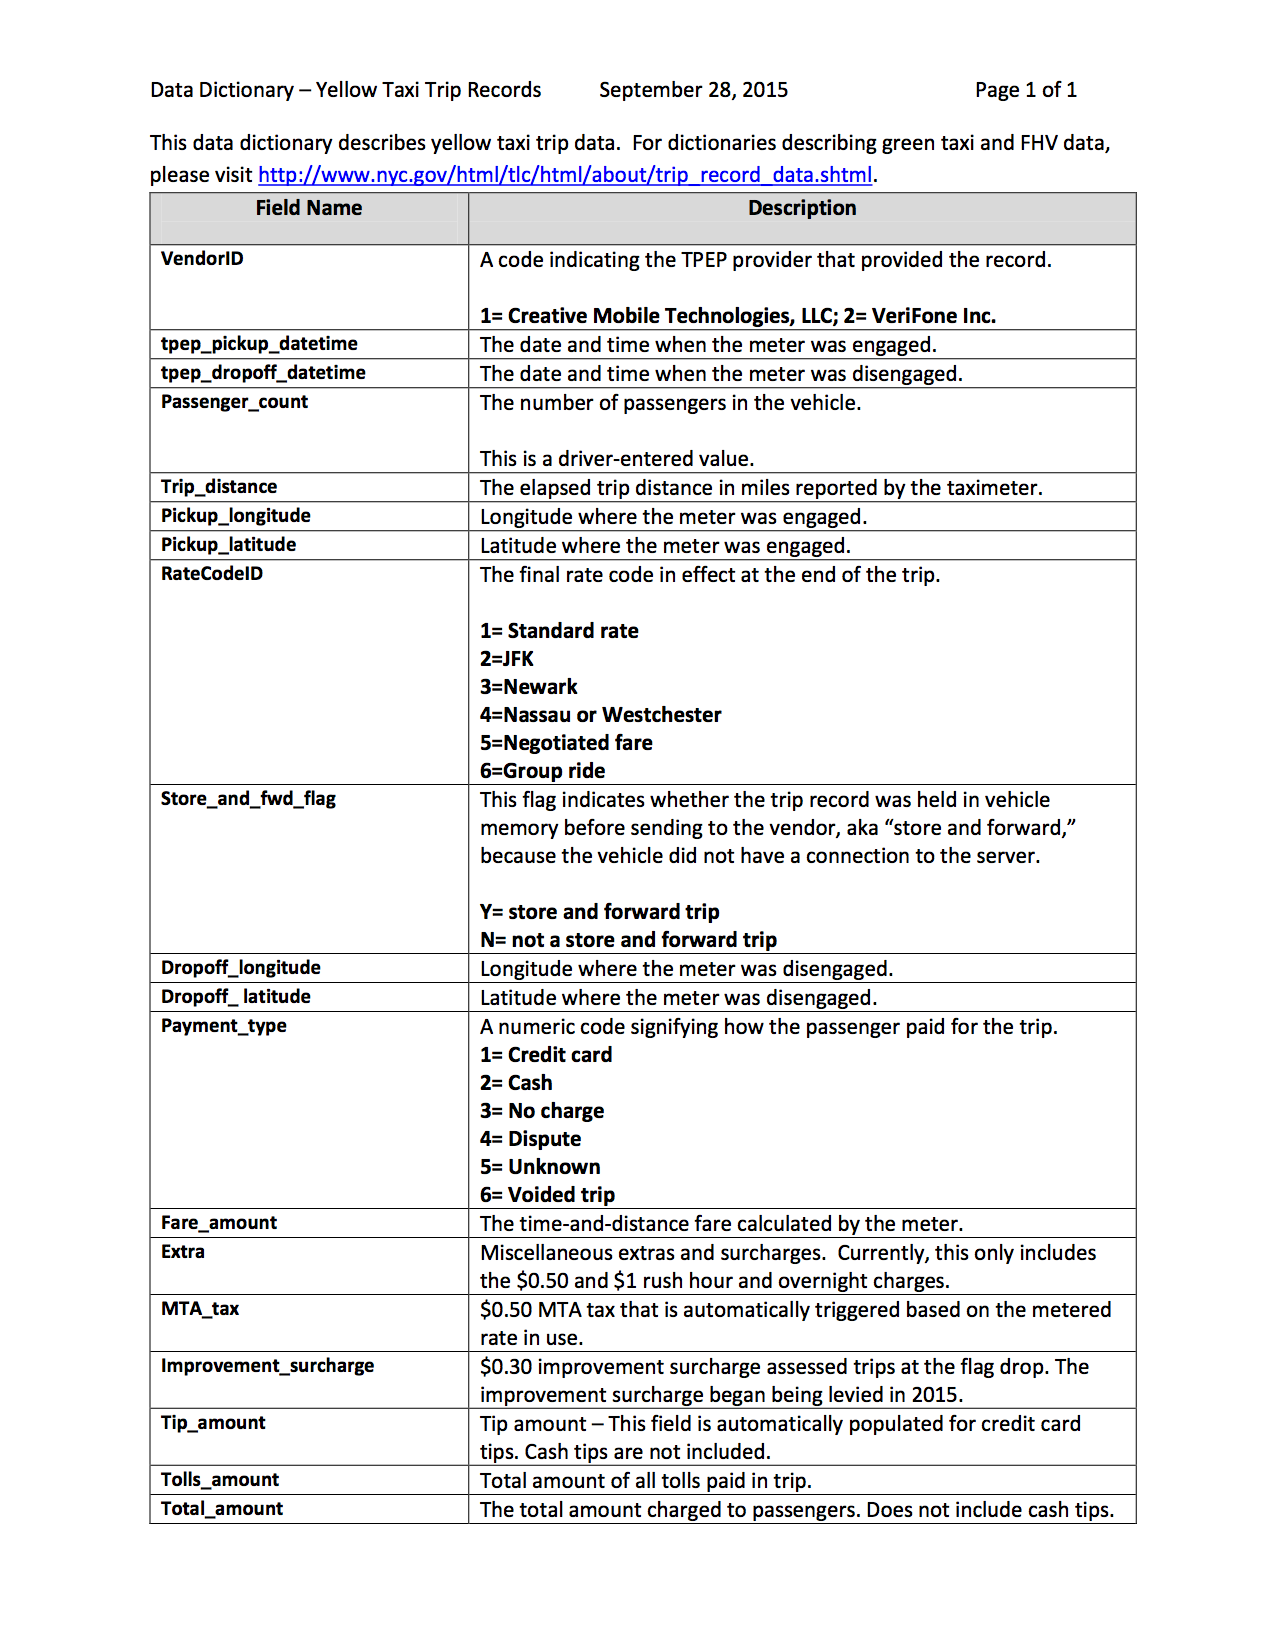
\includegraphics[width=6.38in]{figure/data_dictionary_trip_records_yellow} 

}

\caption{Data Dictionary -- Yellow Taxi Trips Records}\label{fig:datadic}
\end{figure}
\chapter{Freedom of Information Law
Request}\label{freedom-of-information-law-request}

We submitted this FOIL Request to seek answers of the questions listed
below to better analyze the yellow taxi data.
\begin{figure}[h]

{\centering 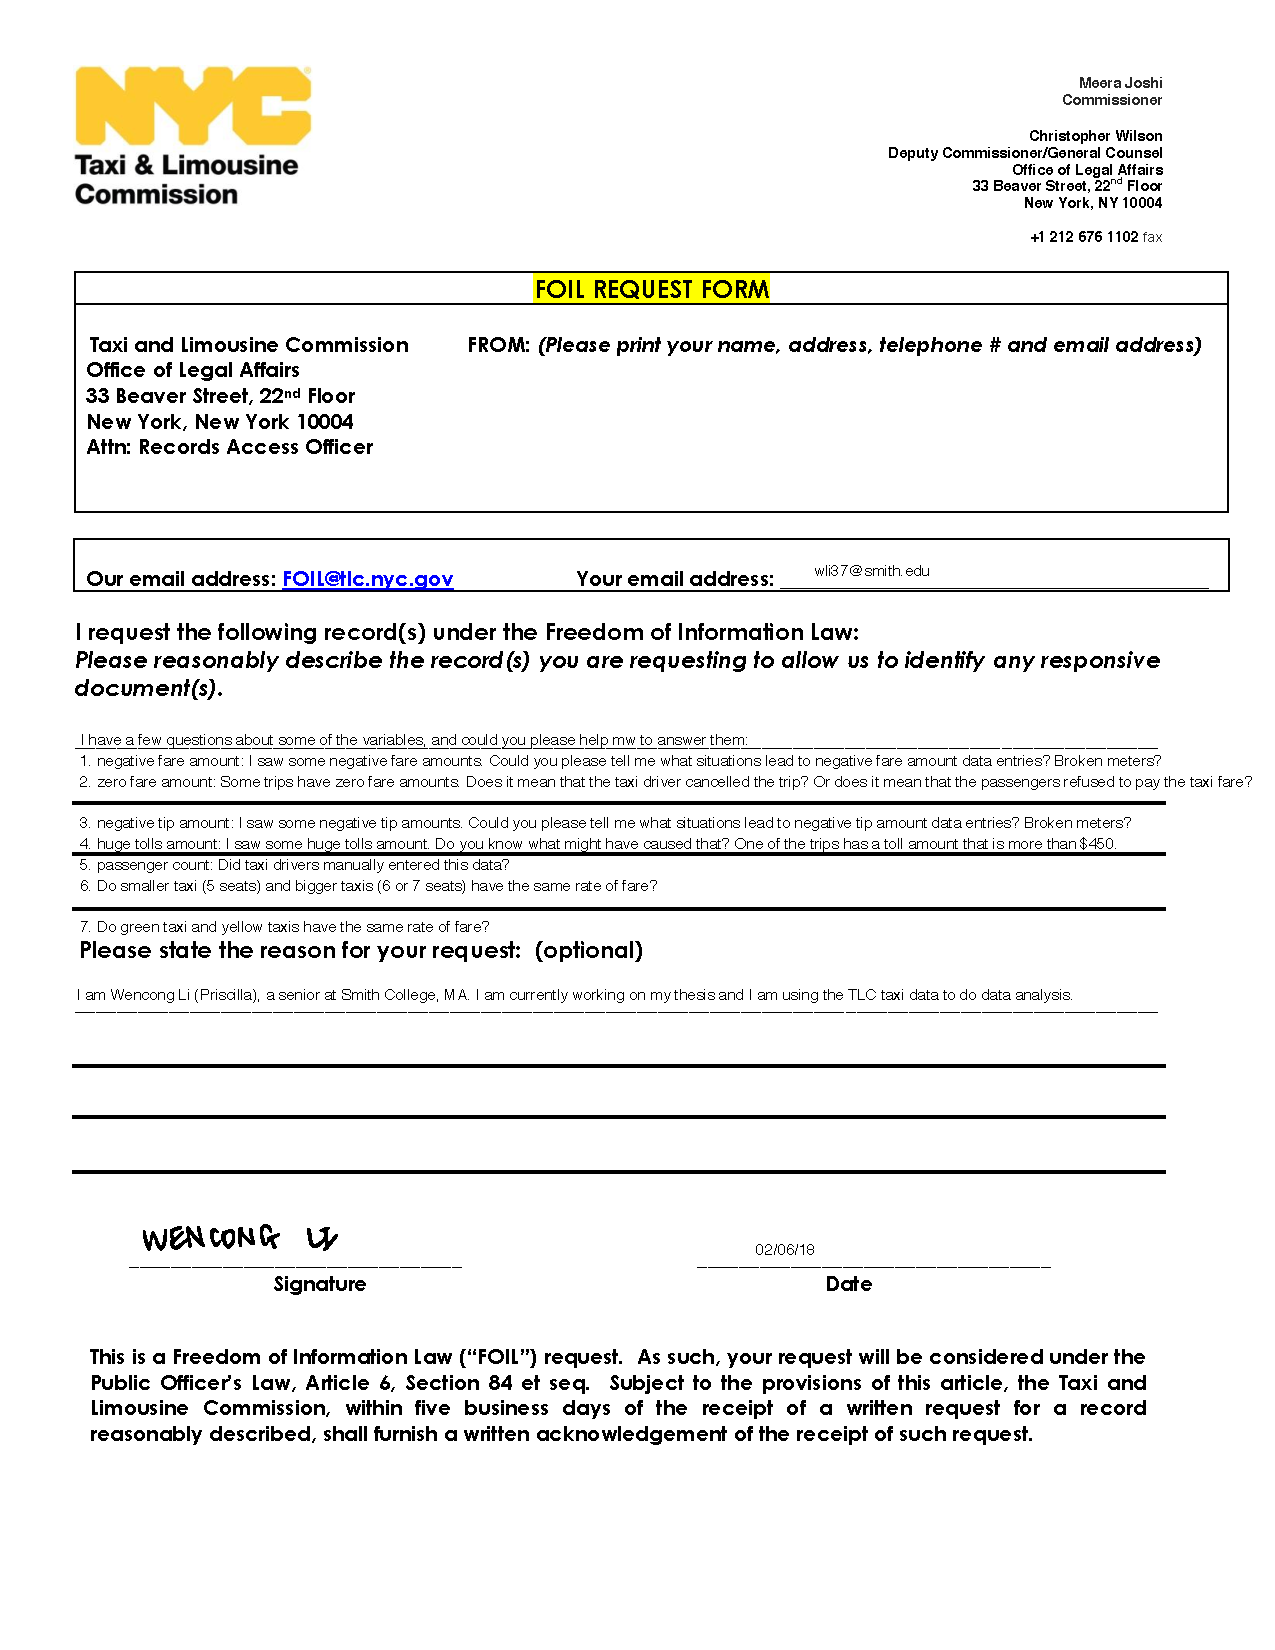
\includegraphics[width=6.38in]{figure/appendix_foil_form_doc} 

}

\caption{Freedom of Information Law Request}\label{fig:foil}
\end{figure}
\chapter{NOAA Climate Data Request}\label{noaa-climate-data-request}

We submitted the NOAA Climate Data Request to get access to 2017 New
York City weather data.
\begin{figure}[h]

{\centering 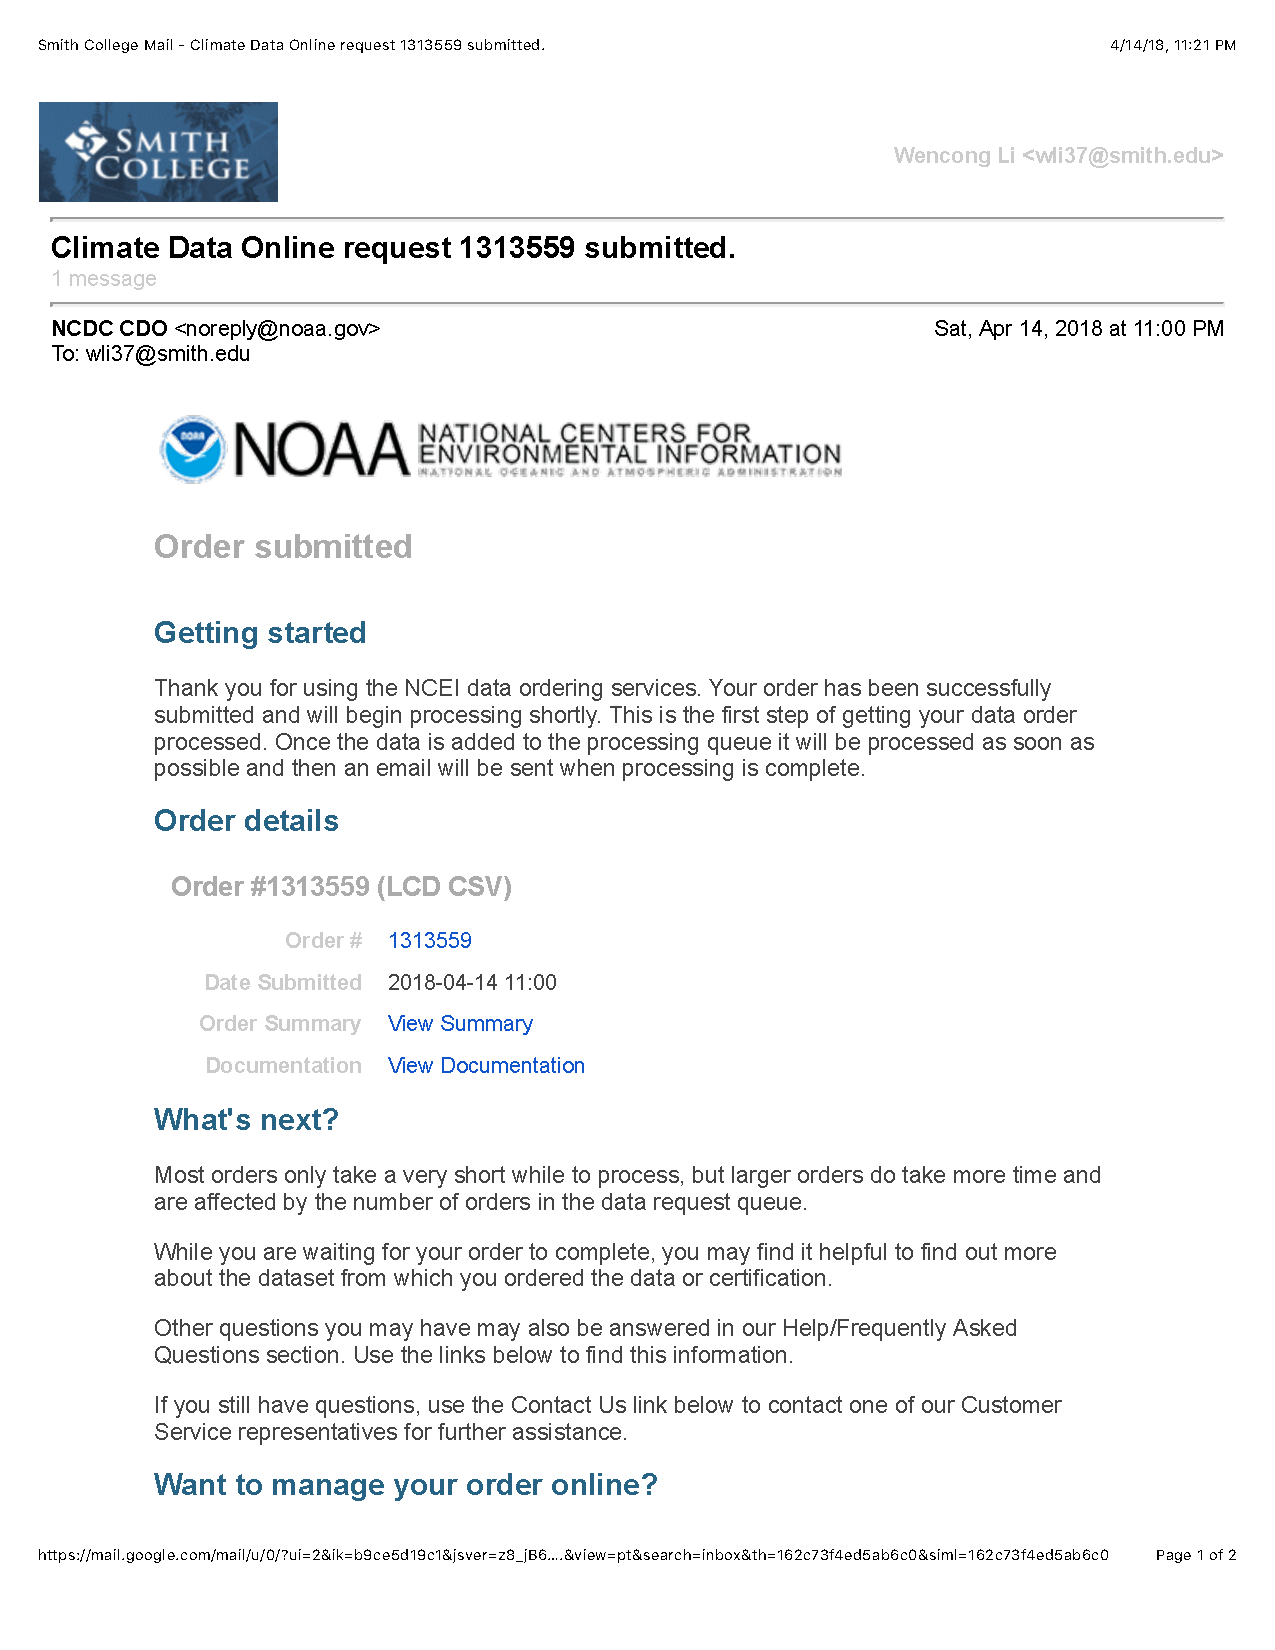
\includegraphics[width=5.8in]{figure/app_noaa_request} 

}

\caption{NOAA Climate Data Request}\label{fig:noaareq}
\end{figure}
The NOAA Climate Data Order Completion Notification grants me rights the
access to 2017 New York City weather data.
\begin{figure}[h]

{\centering 
\includegraphics[width=5.8in]{figure/app_noaa_com} 

}

\caption{NOAA Climate Data Order Compeletion}\label{fig:noaacom}
\end{figure}
\backmatter

\chapter*{References}\label{references}
\addcontentsline{toc}{chapter}{References}

\markboth{References}{References}

\noindent

\setlength{\parindent}{-0.20in} \setlength{\leftskip}{0.20in}
\setlength{\parskip}{8pt}

\hypertarget{refs}{}
\hypertarget{ref-pkgetl}{}
Baumer, B. S. (2017). A grammar for reproducible and painless
extract-transform-load operations on medium data. Retrieved from
\url{https://arxiv.org/abs/1708.07073}

\hypertarget{ref-baumer2014}{}
Baumer, B., Cetinkaya-Rundel, M., Bray, A., Loi, L., \& Horton, N. J.
(2014). R markdown: Integrating a reproducible analysis tool into
introductory statistics. \emph{TISE}.

\hypertarget{ref-nytimes2018}{}
Board, T. E. (2018). What Will New York Do About Its Uber Problem?
\emph{The New York Times}.

\hypertarget{ref-pkgleaflet}{}
Cheng, J., Karambelkar, B., \& Xie, Y. (2017). \emph{Leaflet: Create
interactive web maps with the javascript 'leaflet' library}. Retrieved
from \url{https://CRAN.R-project.org/package=leaflet}

\hypertarget{ref-pkgdatatable}{}
Dowle, M., \& Srinivasan, A. (2017). \emph{Data.table: Extension of
`data.frame`}. Retrieved from
\url{https://CRAN.R-project.org/package=data.table}

\hypertarget{ref-noaa}{}
Environmental Information Staff, N. C. for. (2018). Climate Data Online.
National Centers for Environmental Information. Retrieved from
\url{https://www.ncdc.noaa.gov/cdo-web/}

\hypertarget{ref-uber538}{}
FiveThirtyEight. (2015, September). Uber TLC FOIL Response. Retrieved
from \url{https://github.com/fivethirtyeight/uber-tlc-foil-response}

\hypertarget{ref-furfaro2016}{}
Furfaro, D., Cohen, S., \& Fears, D. (2016, December). NYC is already
tired of Christmas and Donald Trump. New York Post. Retrieved from
\url{https://nypost.com/2016/12/01/nyc-is-already-tired-of-christmas-and-donald-trump/}

\hypertarget{ref-pkglubridate}{}
Grolemund, G., \& Wickham, H. (2011). Dates and times made easy with
lubridate. \emph{Journal of Statistical Software}, \emph{40}(3), 1--25.
Retrieved from \url{http://www.jstatsoft.org/v40/i03/}

\hypertarget{ref-andrew2016}{}
Hawkins, A. J. (2016, September). Yellow taxis have a new weapon in
their war against uber: Gadgets. The Verge. Retrieved from
\url{https://www.theverge.com/2016/9/26/13035642/nyc-taxi-cab-android-touchscreen-tablet-verifone}

\hypertarget{ref-pkgrlang}{}
Henry, L., \& Wickham, H. (2018). \emph{Rlang: Functions for base types
and core r and 'tidyverse' features}. Retrieved from
\url{https://CRAN.R-project.org/package=rlang}

\hypertarget{ref-hu2017}{}
Hu, W. (2017, January). Yellow Cab, Long a Fixture of City Life, Is for
Many a Thing of the Past. The New York Times. Retrieved from
\url{https://www.nytimes.com/2017/01/15/nyregion/yellow-cab-long-a-fixture-of-city-life-is-for-many-a-thing-of-the-past.html}

\hypertarget{ref-citylab}{}
Jaffe, E. (2014, October). Why New Yorkers Can't Find a Taxi When It
Rains. CITYLAB. Retrieved from
\url{https://www.citylab.com/environment/2014/10/why-new-yorkers-cant-find-a-taxi-when-it-rains/381652/}

\hypertarget{ref-foirequest}{}
Li, W. (2018, February). FOIL request. NYC TLC.

\hypertarget{ref-pkgnyctaxi}{}
Li, W. P., Baumer, B., \& Trang Le. (2017). \emph{Nyctaxi: Accessing new
york city taxi data}. Retrieved from
\url{http://github.com/beanumber/nyctaxi}

\hypertarget{ref-pkgDBI}{}
R Special Interest Group on Databases (R-SIG-DB), Wickham, H., \&
Müller, K. (2018). \emph{DBI: R database interface}. Retrieved from
\url{https://CRAN.R-project.org/package=DBI}

\hypertarget{ref-reaney2009}{}
Reaney, P. (2009, June). New York Drivers Named Most Aggressive, Angry
in U.S. Reuters. Retrieved from
\url{https://www.reuters.com/article/us-driving-roadrage-life/new-york-drivers-named-most-aggressive-angry-in-u-s-idUSTRE55F1J720090616}

\hypertarget{ref-schneider2015}{}
Schneider, T. W. (2015, November). Analyzing 1.1 Billion NYC Taxi and
Uber Trips, with a Vengeance. Todd W. Schneider. Retrieved from
\url{http://toddwschneider.com/posts/analyzing-1-1-billion-nyc-taxi-and-uber-trips-with-a-vengeance/}

\hypertarget{ref-pkgthesisdown}{}
Solomon, N. (2016). \emph{Thesisdown: An updated r markdown thesis
template using the bookdown package}.

\hypertarget{ref-cran}{}
Staff, C. (1993). The Comprehensive R Archive Network. Retrieved from
\url{https://cran.r-project.org/index.html}

\hypertarget{ref-uberx}{}
Staff, H. (2018, January). Uber's 4 Basic Level of Service. HyreCar.
Retrieved from
\url{https://hyrecar.com/blog/difference-between-uber-cars/}

\hypertarget{ref-datalyft}{}
Staff, N. O. (2015a). LYFT Data. NYC OpenData. Retrieved from
\url{https://data.cityofnewyork.us/Transportation/LYFT-Data/juxc-sutg/data}

\hypertarget{ref-datauberweek}{}
Staff, N. O. (2015b). Uber Trips NYC 2016. NYC OpenData. Retrieved from
\url{https://data.cityofnewyork.us/Transportation/Uber-Trips-NYC-2016/gt3n-7ri6/data}

\hypertarget{ref-tlcfarerate}{}
Staff, N. T. (1996). NYC tlc Taxicab Rate of Fare. NYC TLC. Retrieved
from \url{http://www.nyc.gov/html/tlc/html/passenger/taxicab_rate.shtml}

\hypertarget{ref-datayellowmonth}{}
Staff, N. T. (2009a). TLC Aggregated Reports. NYC Taxi \& Limousine
Commission. Retrieved from
\url{http://www.nyc.gov/html/tlc/html/technology/aggregated_data.shtml}

\hypertarget{ref-datayellow}{}
Staff, N. T. (2009b). TLC Trip Record Data. NYC Taxi \& Limousine
Commission. Retrieved from
\url{http://www.nyc.gov/html/tlc/html/about/trip_record_data.shtml}

\hypertarget{ref-datauber}{}
Staff, N. T. (2009c). TLC Trip Record Data. NYC Taxi \& Limousine
Commission. Retrieved from
\url{http://www.nyc.gov/html/tlc/html/about/trip_record_data.shtml}

\hypertarget{ref-greentaxi}{}
Staff, N. T. (2009d). Your guide to Boro Taxis. NYC Taxi \& Limousine
Commission. Retrieved from
\url{http://www.nyc.gov/html/tlc/html/passenger/shl_passenger.shtml}

\hypertarget{ref-nyctlc}{}
Staff, N. T. (2018). NYC Taxi \& Limousine Commission. NYC Taxi \&
Limousine Commission. Retrieved from
\url{http://www.nyc.gov/html/tlc/html/home/home.shtml}

\hypertarget{ref-uberweb}{}
Staff, U. (2009, March). Uber Technologies Inc. Retrieved from
\url{https://www.uber.com}

\hypertarget{ref-sugar2017}{}
Sugar, R. (2017, January). Uber and Lyft cars now outnumber yellow cabs
in NYC 4 to 1. Curbed New York. Retrieved from
\url{https://ny.curbed.com/2017/1/17/14296892/yellow-taxi-nyc-uber-lyft-via-numbers}

\hypertarget{ref-ubernyc}{}
Uber Moves New York City. (2015, November). Uber. Retrieved from
\url{https://www.uber.com/cities/new-york/}

\hypertarget{ref-guerrini2015}{}
Vsevolod Salnikov, A. N., Renaud Lambiotte. (2015). OpenStreetCab:
Exploiting Taxi Mobility Patterns in New York City to Reduce Commuter
Costs.

\hypertarget{ref-emma2017}{}
Whitford, E. (2017, October). Daily Uber Trips Have Officially
Outstripped Taxi Trips. Gothamist. Retrieved from
\url{http://gothamist.com/2017/10/13/uber_taxis_nyc.php}

\hypertarget{ref-pkgstringr}{}
Wickham, H. (2018). \emph{Stringr: Simple, consistent wrappers for
common string operations}. Retrieved from
\url{https://CRAN.R-project.org/package=stringr}

\hypertarget{ref-pkgdplyr}{}
Wickham, H., Francois, R., Henry, L., \& Müller, K. (2017). \emph{Dplyr:
A grammar of data manipulation}. Retrieved from
\url{https://CRAN.R-project.org/package=dplyr}

\hypertarget{ref-pkgreadr}{}
Wickham, H., Hester, J., \& Francois, R. (2017). \emph{Readr: Read
rectangular text data}. Retrieved from
\url{https://CRAN.R-project.org/package=readr}

\hypertarget{ref-pkgknitr}{}
Xie, Y. (2018). \emph{Knitr: A general-purpose package for dynamic
report generation in r}. Retrieved from
\url{https://CRAN.R-project.org/package=knitr}

\hypertarget{ref-zhang2017}{}
Zhang, W. (2017, May). Improving access to open-source data about the
nyc bike sharing system (Citi Bike). Smith College.

\hypertarget{ref-vega2017}{}
Zhnag, W. (2017). Improving access to open-source data about the NYC
bike sharing system (citi bike). \emph{Smith College Scholar Works}.


% Index?

\end{document}
